%%%%%%%% ICML 2026 EXAMPLE LATEX SUBMISSION FILE %%%%%%%%%%%%%%%%%

\documentclass{article}

% Recommended, but optional, packages for figures and better typesetting:
\usepackage{microtype}
\usepackage{graphicx}
\usepackage{subcaption}
\usepackage{booktabs} % for professional tables

% hyperref makes hyperlinks in the resulting PDF.
% If your build breaks (sometimes temporarily if a hyperlink spans a page)
% please comment out the following usepackage line and replace
% \usepackage{icml2026} with \usepackage[nohyperref]{icml2026} above.
\usepackage{hyperref}

\usepackage{multirow}
\usepackage{bm}
\usepackage{colortbl}
\usepackage{xcolor}
\definecolor{grayhighlight}{gray}{0.9} % 定义浅灰色
% Attempt to make hyperref and algorithmic work together better:
\newcommand{\theHalgorithm}{\arabic{algorithm}}

% Use the following line for the initial blind version submitted for review:
\usepackage[preprint]{icml2026}
% 尝试清空预印本的文字变量（如果模板使用此变量）
\newcommand{\icmlpreprinttext}{}
\renewcommand{\icmlpreprinttext}{}
% For preprint, use
% \usepackage[preprint]{icml2026}

% If accepted, instead use the following line for the camera-ready submission:
% \usepackage[accepted]{icml2026}

\usepackage{amsmath}
\usepackage{amssymb}
\usepackage{mathtools}
\usepackage{amsthm}


% if you use cleveref..
\usepackage[capitalize,noabbrev]{cleveref}

%%%%%%%%%%%%%%%%%%%%%%%%%%%%%%%%
% THEOREMS
%%%%%%%%%%%%%%%%%%%%%%%%%%%%%%%%
\theoremstyle{plain}
\newtheorem{theorem}{Theorem}[section]
\newtheorem{proposition}[theorem]{Proposition}
\newtheorem{lemma}[theorem]{Lemma}
\newtheorem{corollary}[theorem]{Corollary}
\theoremstyle{definition}
\newtheorem{definition}[theorem]{Definition}
\newtheorem{assumption}[theorem]{Assumption}
\theoremstyle{remark}
\newtheorem{remark}[theorem]{Remark}

% Todonotes is useful during development; simply uncomment the next line
%    and comment out the line below the next line to turn off comments
%\usepackage[disable,textsize=tiny]{todonotes}
\usepackage[textsize=tiny]{todonotes}
\usepackage{bm}
% The \icmltitle you define below is probably too long as a header.
% Therefore, a short form for the running title is supplied here:
\icmltitlerunning{ Optimistic Distributionally Robust Policy Optimization for Off-Policy Generative Recommendation}
\setlength{\abovedisplayskip}{3pt}
\setlength{\belowdisplayskip}{3pt}

\usepackage[absolute,overlay]{textpos}

\usepackage{fancyhdr}
\pagestyle{fancy}

\begin{document}


\begin{textblock*}{\paperwidth}(1.5cm, 1.2cm)

\includegraphics[height=1.5cm]{figures/logo_v2.png} % 请确保目录下有 logo.png
\end{textblock*}

\twocolumn[
  \icmltitle{Breaking the Curse of Repulsion: Optimistic Distributionally Robust Policy Optimization}

  % It is OKAY to include author information, even for blind submissions: the
  % style file will automatically remove it for you unless you've provided
  % the [accepted] option to the icml2026 package.

  % List of affiliations: The first argument should be a (short) identifier you
  % will use later to specify author affiliations Academic affiliations
  % should list Department, University, City, Region, Country Industry
  % affiliations should list Company, City, Region, Country

  % You can specify symbols, otherwise they are numbered in order. Ideally, you
  % should not use this facility. Affiliations will be numbered in order of
  % appearance and this is the preferred way.
  \icmlsetsymbol{equal}{*}

  \begin{icmlauthorlist}
    \icmlauthor{Jie Jiang}{equal,comp}
    \icmlauthor{Yusen Huo}{equal,comp}
    \icmlauthor{Changping Wang}{comp}
    \icmlauthor{Jun Zhang}{comp}
  \end{icmlauthorlist}
  \icmlaffiliation{comp}{Tencent Inc, China}

  \icmlcorrespondingauthor{Jun Zhang}{neoxzhang@tencent.com}

  % You may provide any keywords that you find helpful for describing your
  % paper; these are used to populate the "keywords" metadata in the PDF but
  % will not be shown in the document
  \icmlkeywords{Reinforcement Learning, Recommendation System, DRPO}

  \vskip 0.3in
]

% this must go after the closing bracket ] following \twocolumn[ ...

% This command actually creates the footnote in the first column listing the
% affiliations and the copyright notice. The command takes one argument, which
% is text to display at the start of the footnote. The \icmlEqualContribution
% command is standard text for equal contribution. Remove it (just {}) if you
% do not need this facility.

% Use ONE of the following lines. DO NOT remove the command.
% If you have no special notice, KEEP empty braces:
% \printAffiliationsAndNotice{}  % no special notice (required even if empty)
% Or, if applicable, use the standard equal contribution text:

\printAffiliationsAndNotice{\icmlEqualContribution}


\begin{abstract}
Off-policy policy optimization reuses historical behavior, including negative-advantage samples that suppress known failures. We show that repeated reuse can turn this useful signal into excessive repulsion. As the learner moves away from a historical negative action, subsequent negative updates make that action increasingly remote under the current policy while preserving or amplifying its influence. We formalize this far-field repulsive dynamic and show a transition from useful extrapolation to instability: moderate negative feedback can improve upon policies trained only on positive-advantage samples, whereas excessive far-field repulsion leads to persistent drift or the loss of finite stable equilibria. The resulting control problem is not merely distance weighting: learner-relative remoteness is nonlinear, corresponding to squared standardized distance for Gaussian policies and surprisal for categorical policies, while the local utility of remote negative feedback decays. Motivated by this principle, DRPO applies nonlinear remoteness-aware attenuation to retain informative near-field updates while suppressing far-field repulsion. Controlled experiments identify the causal mechanism, and D4RL locomotion and Countdown arithmetic generation show that the control remains beneficial in realistic external tasks.
 % while generalizing effectively to broader continuous control tasks.


\end{abstract}

\section{Introduction}
\label{sec:intro}

Off-policy policy optimization improves a current policy using behavior collected by earlier, stale, or heterogeneous policies. This paradigm is essential in settings where fresh interaction is costly, slow, or unavailable, including offline reinforcement learning, replay-based control, recommender systems, and the post-training of generative models. By reusing historical experience, it can reduce exploration cost, exploit data accumulated across policy iterations, and enable policy improvement without relying exclusively on new on-policy trajectories. This benefit, however, creates a distinctive learning problem: the policy continues to evolve while the data being optimized remain fixed. Understanding how this growing mismatch changes the influence of historical feedback is therefore central to building stable and effective off-policy learning algorithms.


Historical datasets, however, contain more than successful behavior to imitate. They also record suboptimal and failed actions that reveal which decisions should be suppressed. Policy-based methods exploit this distinction through signed feedback: positive updates increase the likelihood of successful behavior, whereas negative updates reduce the probability of known failures. Prior work has shown that policy-learning objectives can retain or reweight both positive and negative feedback rather than treating all non-positive samples identically \citep{peng2019advantage,kostrikov2021offline,nair2020awac,arnal2025asymmetric,leroux2025tapered}. Building on these observations, we view positive and negative feedback as complementary signals: positive updates provide attraction toward observed successes, while negative updates encode boundaries and failure information that positive imitation alone cannot express. We therefore ask how this information can be retained without allowing repeated historical reuse to turn negative feedback into excessive repulsion.

Against this background, we identify a self-amplifying far-field dynamic in repeated off-policy updates. A negative update pushes the learner away from a fixed historical action, increasing its learner-relative distance or surprisal. This increased remoteness can in turn strengthen—or prevent the decay of—the action’s subsequent negative influence, causing repeated reuse to drive it progressively farther from the current policy. The precise amplification law depends on the policy family: continuous Gaussian policies can exhibit distance-dependent score growth, whereas categorical policies exhibit persistent suppression toward the support boundary. Thus, the danger lies not only in where a negative sample starts, but in how its influence evolves through repeated repulsion.

Prior work has stabilized off-policy learning through filtering, importance weighting, clipping, behavior regularization, and tapered negative updates \citep{peng2019advantage,fujimoto2019off,kumar2020conservative,schulman2017proximal,arnal2025asymmetric,leroux2025tapered}. These methods demonstrate the value of nonuniform control, but they do not isolate whether learner-relative remoteness itself generates a self-amplifying repulsive dynamic. In realistic data, sample quality, advantage magnitude, rarity, and policy distance are entangled. We disentangle these factors through matched controlled environments and causally test the pathway from remoteness, to amplified negative influence, to policy drift and collapse.



To characterize this process, we develop an aggregate theory of repulsive policy updates. The analysis shows that moderate negative feedback can improve upon what positive updates alone attain, whereas repeated far-field repulsion can progressively distort the aggregate equilibrium and ultimately eliminate a finite solution. This dynamic motivates DRPO, a learner-relative nonlinear control of negative updates. DRPO measures distance or surprisal under the evolving policy and applies an attenuation that is mild locally but increases nonlinearly in the far field. The resulting exponential envelope preserves informative local repulsion while dominating the far-field tail generated by the self-amplifying dynamics.

We evaluate the resulting theory and method through a layered empirical program. Controlled continuous and categorical experiments test the predicted transition from useful negative feedback to far-field instability and assess whether learner-relative nonlinear attenuation preserves the former while preventing the latter. We then examine whether the same mechanisms appear in continuous-control and sequence-generation tasks. Together, these experiments connect the proposed dynamics to controlled causal evidence, method behavior, and external task performance.

Our contributions are summarized as follows:

\begin{itemize}\setlength{\itemsep}{0pt}\setlength{\parskip}{0pt}\setlength{\parsep}{0pt}
    \item we formulate repeated off-policy negative updates as learner-relative repulsive dynamics and develop an aggregate theory that characterizes stable extrapolation, boundary approach, and the loss of a finite equilibrium.

    \item we construct matched controlled environments and targeted near–far interventions that separate sample quality from learner-relative remoteness and causally trace amplified repulsion to policy drift and collapse.

    \item we propose DRPO, a learner-relative nonlinear attenuation of negative updates that uses distance or surprisal to preserve informative local feedback while suppressing the self-amplifying far-field tail.

    \item we evaluate the resulting theory and method across controlled continuous and categorical settings, together with external continuous-control and sequence-generation tasks.
    % and generalizes effectively to broader continuous control tasks.
\end{itemize}


% ------------------------------------------------------------------
% SECTION 2: PRELIMINARIES
% ------------------------------------------------------------------
\section{Related Work}
\label{sec:related_work}

\textbf{Learning from Negative or Suboptimal Behavior.}
A broad line of policy-learning methods distinguishes behavior according to its estimated quality. Advantage-weighted regression and related actor-fitting objectives emphasize actions with higher estimated advantages, whereas positive-only or filtering approaches remove some or all negative updates \citep{peng2019advantage,kostrikov2021offline,nair2020awac}. Other off-policy objectives explicitly retain or rebalance negative feedback instead of discarding it wholesale \citep{arnal2025asymmetric,leroux2025tapered}. Together, these findings establish that negative feedback can be informative rather than merely noisy, while leaving open how its benefits can be retained without introducing harmful optimization dynamics.

\textbf{Off-Policy, Stale, and Learner-Relative Updates.}
This challenge becomes particularly important under off-policy reuse, where historical behavior remains fixed while the learner continues to change. Off-policy methods commonly control behavior--learner mismatch through importance weighting, clipping, trust regions, and behavior regularization \citep{fujimoto2019off,schulman2017proximal,kumar2020conservative}. More recent methods, including TOPR and asymmetric off-policy objectives, further attenuate or rebalance negative behavior under the current policy, making the update explicitly learner-relative \citep{arnal2025asymmetric,leroux2025tapered}. These works establish that distance-related information can guide selective control, but largely treat remoteness as a static weighting signal and often study it together with sample quality or advantage magnitude. They therefore leave unresolved how repeated negative updates themselves increase remoteness, alter subsequent influence, and form a feedback process that can drive policy drift or collapse. This perspective is complementary to conservative offline RL, which primarily controls value extrapolation or policy support, whereas we study the evolving dynamics of signed actor updates on fixed historical behavior.
% ------------------------------------------------------------------
% SECTION 2: PRELIMINARIES
% ------------------------------------------------------------------

\section{Problem Setup}
\label{sec:problem_setup}

% ------------------------------------------------------------------
% SECTION 2: PRELIMINARIES
% ------------------------------------------------------------------

\subsection{Off-Policy Signed Actor Updates}

We consider policy optimization from a historical update distribution
$\nu$ over state--action pairs, which may represent an offline dataset,
a replay buffer, or trajectories collected by earlier or stale behavior
policies. Let $\pi_\theta(a \mid s)$ denote the current policy and let
$\widehat{A}(s,a)$ denote the advantage-like signal used by the actor
update. During an actor step, the update distribution and the associated
advantage estimates are treated as fixed with respect to $\theta$. The
resulting empirical actor field is
\begin{equation}
    \mathbf{F}(\theta)
    =
    \mathbb{E}_{(s,a)\sim\nu}
    \left[
        \widehat{A}(s,a)
        \nabla_\theta \log \pi_\theta(a \mid s)
    \right],
    \label{eq:empirical_actor_field}
\end{equation}
with the corresponding update
$\theta_{t+1}=\theta_t+\eta\mathbf{F}(\theta_t)$.
Equation~\eqref{eq:empirical_actor_field} characterizes the actor-side
dynamics induced by repeatedly reusing historical feedback. It is not
assumed to equal the exact on-policy policy gradient, because the update
distribution $\nu$ may differ from the state--action distribution of the
current policy.

To separate favorable and unfavorable feedback, we define
\begin{equation}
\begin{aligned}
    \widehat{A}^{+}(s,a)
    &= \max\{\widehat{A}(s,a),0\}, \\
    \widehat{A}^{-}(s,a)
    &= \max\{-\widehat{A}(s,a),0\}.
\end{aligned}
\end{equation}
The actor field can then be decomposed into positive and negative
components:
\begin{equation}
\begin{aligned}
    \mathbf{F}(\theta)
    ={}&
    \mathbb{E}_{\nu}
    \left[
        \widehat{A}^{+}(s,a)
        \nabla_\theta \log \pi_\theta(a \mid s)
    \right] \\
    &-
    \mathbb{E}_{\nu}
    \left[
        \widehat{A}^{-}(s,a)
        \nabla_\theta \log \pi_\theta(a \mid s)
    \right].
\end{aligned}
\label{eq:signed_actor_decomposition}
\end{equation}
For a negative sample, the update magnitude factorizes as
$\widehat{A}^{-}(s,a)
\lVert\nabla_\theta \log \pi_\theta(a \mid s)\rVert$,
separating the severity of its estimated disadvantage from its
learner-relative policy geometry.

% ------------------------------------------------------------------
% SECTION 3: THEORETICAL FRAMEWORK
% ------------------------------------------------------------------
\section{Far-Field Dynamics of Historical Policy Updates}
\label{sec:theory}

We study how learner-relative remoteness shapes signed policy updates when
historical behavior is reused. We first characterize, in policy-output
coordinates, how the remoteness of a sample determines the strength of its
score contribution. We then show how repeated reuse turns this static
geometry into a dynamic feedback process: positive samples become
self-attenuating as the learner approaches them, whereas negative samples
become self-amplifying as the learner moves away. Finally, we analyze how
these local effects aggregate into finite stable equilibria, persistent
drift, or instability, and derive their specific manifestations in
Gaussian and categorical policies.

\subsection{Learner-Relative Remoteness and Update Strength}
\label{sec:distance_strength}

To isolate the action-side geometry, we fix a context $s$ and write
$u$ for the policy-output coordinates at that context. For a historical
action $a$, we define its learner-relative remoteness as
\begin{equation}
    D_u(a)
    =
    -\log \pi_u(a).
    \label{eq:learner_relative_remoteness}
\end{equation}
For a categorical policy, $D_u(a)$ is the surprisal of the selected
action. For a Gaussian policy, it equals a scale-dependent constant plus
one half of the squared Mahalanobis distance from the policy mean.
Thus, $D_u(a)$ measures how unlikely the historical action is under the
current learner, rather than defining a metric in the action space.

We measure the corresponding squared score norm by
\begin{equation}
    R_u(a)
    =
    \left\|
        \nabla_u \log \pi_u(a)
    \right\|_2^2.
    \label{eq:score_strength}
\end{equation}
A sample with advantage estimate $\widehat{A}(s,a)$ contributes an
output-space update of magnitude
$|\widehat{A}(s,a)|\sqrt{R_u(a)}$.
The following results characterize how learner-relative remoteness
controls this update strength.

\begin{proposition}[Distance-dependent score-function magnitude]
\label{prop:distance_strength}
Fix a context and a historical action $a$.

For a Gaussian policy with mean $\mu$ and fixed covariance
$\Sigma\succ0$, let
\begin{equation}
    C_\Sigma
    =
    \frac{d}{2}\log(2\pi)
    +
    \frac{1}{2}\log|\Sigma|.
\end{equation}
The squared norm of the mean score function satisfies
\begin{equation}
\begin{aligned}
    R_\mu(a)
    &\geq
    2\lambda_{\min}(\Sigma^{-1})
    \bigl(D_\mu(a)-C_\Sigma\bigr), \\
    R_\mu(a)
    &\leq
    2\lambda_{\max}(\Sigma^{-1})
    \bigl(D_\mu(a)-C_\Sigma\bigr).
\end{aligned}
\label{eq:gaussian_distance_response}
\end{equation}
Writing
$d_{\mathrm{Mah}}^2(a,\mu)
=
(a-\mu)^\top\Sigma^{-1}(a-\mu)$
for the squared standardized Mahalanobis distance, we have
$D_\mu(a)-C_\Sigma
=
\frac{1}{2}d_{\mathrm{Mah}}^2(a,\mu)$.
Hence, $R_\mu(a)$ grows quadratically with standardized distance and
linearly with excess negative log-likelihood.

Moreover, along any fixed direction $v\neq0$, with
$a-\mu=rv$,
\begin{equation}
    R_\mu(a)
    =
    2
    \frac{
        v^\top\Sigma^{-2}v
    }{
        v^\top\Sigma^{-1}v
    }
    \bigl(D_\mu(a)-C_\Sigma\bigr).
    \label{eq:gaussian_directional_response}
\end{equation}

For a categorical policy with logits $z$, the selected-logit
score magnitude satisfies
\begin{equation}
    \left|
        \frac{\partial}{\partial z_a}
        \log\pi_z(a)
    \right|
    =
    1-e^{-D_z(a)}.
    \label{eq:categorical_selected_response}
\end{equation}
It therefore increases strictly with surprisal but converges
to the finite limit $1$ as $D_z(a)\rightarrow\infty$.
\end{proposition}

\paragraph{Isotropic covariance.}
If $\Sigma=\sigma^2I$, the directional coefficient is independent
of $v$, and
$R_\mu(a)=2\bigl(D_\mu(a)-C_\sigma\bigr)/\sigma^2$.
Thus, learner-relative remoteness and the squared mean
score-function norm have the same global ordering.

A complete proof, together with bounds on the full categorical
score-function norm, is provided in
Appendix~\ref{app:distance_strength}.

Proposition~\ref{prop:distance_strength} establishes the static
distance--response relation underlying our analysis. For Gaussian
policies, increasing remoteness along any fixed action-space direction
produces an unbounded increase in the mean score-function norm, with a
direction-dependent rate determined by the covariance. For categorical
policies, selected-action suppression increases with surprisal but
saturates at a finite ceiling. The next result shows how historical
reuse turns these static relations into a dynamic feedback process.


\subsection{Self-Amplification under Historical Reuse}
\label{sec:historical_reuse}

The preceding result compares samples at a fixed policy. We now consider
a fixed historical action that is repeatedly reused while the learner
changes. Write
\[
    D(u)=D_u(a),
    \qquad
    R(u)=\left\|\nabla_u D(u)\right\|_2^2,
\]
and consider the repeated single-sample update
\begin{equation}
    u_{t+1}
    =
    u_t
    +
    \eta\widehat{A}
    \nabla_u\log\pi_{u_t}(a)
    =
    u_t
    -
    \eta\widehat{A}
    \nabla_uD(u_t).
    \label{eq:historical_reuse_update}
\end{equation}
Here, the action $a$ and its signed coefficient $\widehat{A}$ are held
fixed over the reuse window.

\begin{theorem}[Self-attenuation and self-amplification under reuse]
\label{thm:reuse_dynamics}
Assume that $D(u)$ is differentiable and convex along the update path,
and define
\[
    D_t=D(u_t),
    \qquad
    R_t=R(u_t).
\]

If $\widehat{A}<0$, then every reuse step satisfies
\begin{equation}
    D_{t+1}
    \geq
    D_t
    +
    \eta|\widehat{A}|R_t,
    \qquad
    R_{t+1}\geq R_t.
    \label{eq:negative_reuse_amplification}
\end{equation}
Thus, negative reuse makes the historical action increasingly remote
while preventing its score-function norm from decreasing.

If $\widehat{A}>0$, and $D$ has an $L$-Lipschitz gradient with
$0<\eta\widehat{A}\leq 1/L$, then
\begin{equation}
    D_{t+1}
    \leq
    D_t
    -
    \frac{\eta\widehat{A}}{2}R_t,
    \qquad
    R_{t+1}\leq R_t.
    \label{eq:positive_reuse_attenuation}
\end{equation}
Thus, positive reuse makes the historical action increasingly compatible
with the learner while attenuating its subsequent score response.
\end{theorem}

A proof is provided in
Appendix~\ref{app:reuse_dynamics}.
The convexity assumption holds, in particular, for fixed-covariance
Gaussian mean coordinates and categorical logits. More generally, for
a regular exponential family in natural coordinates,
\[
    \nabla_u^2D(u)
    =
    \operatorname{Cov}_{\pi_u}[T(a)]
    \succeq0.
\]

Theorem~\ref{thm:reuse_dynamics} distinguishes a one-time distant update
from a historical-reuse feedback loop. A negative sample is first pushed
farther from the learner; the resulting remoteness then preserves or
increases its subsequent score response. Combined with
Proposition~\ref{prop:distance_strength}, this produces unbounded
amplification for fixed-covariance Gaussian mean updates and bounded but
persistent amplification for categorical logits. These per-sample
dynamics do not yet imply global divergence, because positive samples
regain attractive force as the learner moves. We therefore next analyze
their aggregate balance.

\subsection{Aggregate Equilibria under Historical Reuse}
\label{sec:aggregate_equilibria}

The preceding results characterize the repeated influence of an
individual historical action, but do not imply that the full policy must
diverge: as negative repulsion moves the learner, positive samples regain
attractive force. We therefore analyze the aggregate balance between
positive and negative historical updates.

At a fixed context, consider a regular minimal exponential-family policy
\begin{equation}
    \pi_\eta(a)
    =
    h(a)
    \exp
    \left\{
        \eta^\top T(a)
        -
        \psi(\eta)
    \right\},
    \label{eq:exponential_family_policy}
\end{equation}
where $\eta\in\mathcal{H}$ is the natural parameter. Define the effective
positive and negative update masses
\begin{equation}
\begin{aligned}
    p
    &=
    \mathbb{E}_{\nu}
    \left[
        \widehat{A}^{+}(a)
    \right],
    &
    q
    &=
    \mathbb{E}_{\nu}
    \left[
        \widehat{A}^{-}(a)
    \right],
    \\
    p\mathbf{m}_{+}
    &=
    \mathbb{E}_{\nu}
    \left[
        \widehat{A}^{+}(a)T(a)
    \right],
    &
    q\mathbf{m}_{-}
    &=
    \mathbb{E}_{\nu}
    \left[
        \widehat{A}^{-}(a)T(a)
    \right].
\end{aligned}
\label{eq:aggregate_statistics}
\end{equation}
Thus, $p$ and $q$ combine sample frequency, advantage magnitude, and any
fixed sample weighting. The aggregate signed actor field is
\begin{equation}
    \mathbf{F}(\eta)
    =
    p\mathbf{m}_{+}
    -
    q\mathbf{m}_{-}
    -
    (p-q)\nabla\psi(\eta).
    \label{eq:aggregate_signed_field}
\end{equation}

Let
\begin{equation}
    \mathcal{M}
    =
    \left\{
        \nabla\psi(\eta)
        :
        \eta\in\mathcal{H}
    \right\}
\end{equation}
denote the interior mean-parameter space. We assume that $\psi$ is twice
continuously differentiable and strictly convex, and that
$\nabla\psi:\mathcal{H}\rightarrow\mathcal{M}$ is one-to-one and onto.

\begin{theorem}[Aggregate attraction--repulsion equilibria]
\label{thm:aggregate_equilibrium}
Consider the continuous dynamics
$\dot{\eta}=\mathbf{F}(\eta)$
and the discrete update
$\eta_{t+1}=\eta_t+\alpha\mathbf{F}(\eta_t)$, with $\alpha>0$.

\smallskip
\noindent\textbf{Positive-dominant regime $(p>q)$.}
Define the signed target
\begin{equation}
    \mathbf{m}^{\star}
    =
    \frac{
        p\mathbf{m}_{+}
        -
        q\mathbf{m}_{-}
    }{
        p-q
    }.
    \label{eq:signed_target}
\end{equation}
If $\mathbf{m}^{\star}\in\mathcal{M}$, there is a unique finite
equilibrium $\eta^{\star}$ satisfying
$\nabla\psi(\eta^{\star})=\mathbf{m}^{\star}$.
It is locally asymptotically stable under the continuous dynamics and
locally stable under the discrete update for a sufficiently small step
size. When $q>0$,
\begin{equation}
    \mathbf{m}^{\star}
    -
    \mathbf{m}_{+}
    =
    \frac{q}{p-q}
    \left(
        \mathbf{m}_{+}
        -
        \mathbf{m}_{-}
    \right),
    \label{eq:stable_extrapolation_identity}
\end{equation}
so negative feedback moves the equilibrium beyond the Positive-only
target in the direction away from the negative moment. As
$\mathbf{m}^{\star}$ approaches the boundary of $\mathcal{M}$, the
corresponding natural parameter leaves every compact subset of
$\mathcal{H}$; if $\mathbf{m}^{\star}\notin\mathcal{M}$, no finite
equilibrium exists.

\smallskip
\noindent\textbf{Critical regime $(p=q)$.}
The field becomes the constant
$p(\mathbf{m}_{+}-\mathbf{m}_{-})$.
If $\mathbf{m}_{+}\neq\mathbf{m}_{-}$, the policy exhibits persistent
drift with no finite equilibrium. If
$\mathbf{m}_{+}=\mathbf{m}_{-}$, every point is stationary, but none is
an isolated asymptotically stable equilibrium.

\smallskip
\noindent\textbf{Negative-dominant regime $(p<q)$.}
Any finite stationary point is unstable under both the continuous
dynamics and every discrete update with $\alpha>0$. Hence, this regime
admits no locally asymptotically stable finite equilibrium.
\end{theorem}

The derivation and proof, including the exact discrete-time step-size
condition, are provided in
Appendix~\ref{app:aggregate_equilibrium}.
Theorem~\ref{thm:aggregate_equilibrium} converts the preceding
per-sample amplification mechanism into three terminal regimes: finite
stable extrapolation, persistent drift, and instability. The
extrapolation identity is geometric and does not by itself guarantee
improved task utility. We next derive how these regimes appear in
Gaussian and categorical policies.

% ------------------------------------------------------------------
% SECTION 4: METHODOLOGY
% ------------------------------------------------------------------
\subsection{Policy-Family Manifestations of Negative Dominance}
\label{sec:policy_family_manifestations}

Theorem~\ref{thm:aggregate_equilibrium} establishes that negative
dominance, $p<q$, admits no finite stable equilibrium. It does not,
however, determine whether the resulting runaway produces unbounded
sample gradients. This depends on the policy family.

\begin{theorem}[Unbounded Gaussian versus bounded categorical runaway]
\label{thm:policy_family_manifestations}
Assume $p<q$ and let $r=q-p>0$.

\smallskip
\noindent\textbf{Gaussian policy.}
Consider
$\pi_\mu=\mathcal{N}(\mu,\Sigma)$
with fixed $\Sigma\succ0$, and let
$\mu_{+}$ and $\mu_{-}$ denote the positive and negative weighted action
means. Define
\begin{equation}
    \mu^{\dagger}
    =
    \frac{
        q\mu_{-}-p\mu_{+}
    }{
        q-p
    }.
    \label{eq:gaussian_unstable_point}
\end{equation}
The aggregate mean field is
\begin{equation}
    \mathbf{F}_{\mu}(\mu)
    =
    r\Sigma^{-1}
    \left(
        \mu-\mu^{\dagger}
    \right).
    \label{eq:gaussian_negative_dominant_field}
\end{equation}
Unless initialized exactly at the unstable stationary point
$\mu^{\dagger}$, both the continuous dynamics and every discrete update
with step size $\alpha>0$ satisfy
$\|\mu\|_2\rightarrow\infty$. Consequently, for every fixed historical
action $a$,
\begin{equation}
    \left\|
        \nabla_{\mu}\log\pi_{\mu}(a)
    \right\|_2
    =
    \left\|
        \Sigma^{-1}(a-\mu)
    \right\|_2
    \longrightarrow
    \infty.
    \label{eq:gaussian_unbounded_score}
\end{equation}

\smallskip
\noindent\textbf{Categorical policy.}
Consider
$\pi_z=\operatorname{softmax}(z)$
with at least two actions, using the gauge
$\mathbf{1}^{\top}z=0$.
Unless initialized exactly at a finite stationary point, when one
exists, the continuous and discrete aggregate trajectories leave every
compact subset of the logit space, and their probabilities approach the
simplex boundary along a subsequence. Nevertheless, for every action
$a$ and every finite $z$,
\begin{equation}
\begin{aligned}
    \left\|
        \nabla_z\log\pi_z(a)
    \right\|_2^2
    &=
    \left\|
        e_a-\pi_z
    \right\|_2^2 \\
    &\leq
    2
    \left(
        1-\pi_z(a)
    \right)^2
    \leq
    2.
\end{aligned}
\label{eq:categorical_bounded_score}
\end{equation}
Thus, categorical runaway can produce unbounded logits and probability
degeneration, but not an unbounded score-function norm.
\end{theorem}

The proof is provided in
Appendix~\ref{app:policy_family_manifestations}.
Theorem~\ref{thm:policy_family_manifestations} reveals that the same
aggregate instability has different policy-family manifestations.
Gaussian mean runaway converts increasing action separation directly
into unbounded far-field scores. Categorical policies instead approach
the probability-simplex boundary while each sample score remains
bounded. Hence, categorical degeneration is a bounded-gradient boundary
event rather than Gaussian-style gradient explosion.

A learned Gaussian covariance is not required for the unbounded result.
When covariance additionally contracts along a direction that remains
separated from historical negative actions, it further amplifies the
corresponding score. Neither policy-family result alone implies task
performance collapse or a NaN/Inf numerical failure.



\section{DRPO: Smooth Control of Far-Field Repulsion}
\label{sec:drpo}

The analysis in Section~\ref{sec:theory} shows that negative feedback
should not be treated uniformly. Near-field negative samples can retain
useful boundary and corrective information, whereas historical samples
that become increasingly improbable under the current policy can exert
persistent or self-amplifying repulsion. We therefore define DRPO as a
family of signed policy updates that preserves positive updates while
selectively attenuating negative updates according to learner-relative
remoteness, with the goal of retaining local corrective information
without allowing far-field influence to dominate optimization.
\subsection{Remoteness-Controlled Negative Updates}

To operationalize utility, let
$\widehat J_{\mathcal B}(\theta)$
denote an empirical estimate of task performance on an evaluation batch
$\mathcal B$. For a negative sample
$z=(s,a)$, its raw repulsive update is
$g_\theta^-(z)
=
-\widehat A^-(z)\nabla_\theta\log\pi_\theta(a\mid s)$.
Assigning it a weight $w\in[0,1]$ produces the parameter step
$\Delta\theta(z;w)=\eta w g_\theta^-(z)$.
We define the empirical utility of this weighted update as
\begin{equation}
    \widehat{\mathcal U}_{\mathcal B}
    (z;w\mid\theta)
    =
    \widehat J_{\mathcal B}
    \!\left(
        \theta+\Delta\theta(z;w)
    \right)
    -
    \widehat J_{\mathcal B}(\theta).
    \label{eq:empirical_negative_update_utility}
\end{equation}
The corresponding utility-optimal weight is
$\widehat w_{\mathcal U}^{\star}(z\mid\theta)
\in
\arg\max_{w\in[0,1]}
\widehat{\mathcal U}_{\mathcal B}(z;w\mid\theta)$.

The empirical utility measures the practical task effect of the negative
update induced by sample $z$ under the current policy, and may be
positive or negative. When task-aligned gains are outweighed by
far-field drift or support contraction, the utility-optimal weight
shrinks toward zero. Sufficient geometric and curvature conditions are
given in Appendix~\ref{app:negative_update_utility}, consistent with
prior work relating policy discrepancy to replay reliability and
gradient alignment to learning-signal usefulness
\citep{novati2019remember,fakoor2020p3o,du2018adapting}.

where
$D_\theta(s,a)=-\log\pi_\theta(a\mid s)$
is defined in Section~\ref{sec:distance_strength}.
We call this framework DRPO because it makes policy optimization
distributionally robust to increasingly remote historical negative
updates.

For compactness, define the controlled signed coefficient
\begin{equation}
\begin{aligned}
    \widetilde A_\theta(s,a)
    &=
    \widehat A^+(s,a) \\
    &\quad-
    \omega\!\left(D_\theta(s,a)\right)
    \widehat A^-(s,a).
\end{aligned}
\label{eq:drpo_controlled_advantage}
\end{equation}
The resulting DRPO update field is
\begin{equation}
    \mathbf F_{\mathrm{DRPO}}(\theta)
    =
    \mathbb E_{(s,a)\sim\nu}
    \left[
        \widetilde A_\theta(s,a)
        \nabla_\theta
        \log\pi_\theta(a\mid s)
    \right].
    \label{eq:drpo_update_field}
\end{equation}
Thus, DRPO leaves positive updates unchanged, retains nearby negative
feedback, and progressively suppresses negative updates as they become
increasingly remote under the current policy. The remaining question is
how $\omega(D)$ should decay in the far field.

A reciprocal taper need not make the weighted far-field update vanish,
whereas hard filtering removes it through an abrupt discontinuity. We
therefore seek a smooth taper that preserves near-field negative
feedback while driving the far-field contribution to zero.

\subsection{Exponential Remoteness Taper}
\label{sec:exponential_taper}

Negative-update controls can be divided into two classes.
Distance-agnostic controls assign the same coefficient to all negative
samples: uncontrolled updates use unit weight, positive-only learning
removes all negative updates, and global scaling applies a constant
coefficient. Remoteness-aware controls instead vary the weight with
$D_\theta$: a hard cutoff removes all samples beyond a threshold, while
reciprocal and exponential tapers attenuate them progressively. DRPO
uses the exponential form to preserve near-field feedback while driving
far-field influence smoothly to zero.

We instantiate the DRPO weighting function with a thresholded exponential
taper,
\begin{equation}
    \omega_{\mathrm{Exp}}(D)
    =
    \exp
    \left\{
        -\lambda
        \left[
            \frac{D-\tau}{c}
        \right]_{+}
    \right\},
    \label{eq:drpo_exp_weight}
\end{equation}
where $\tau$ marks the onset of far-field control, $c>0$ fixes the
remoteness scale, and $\lambda>0$ controls the decay rate. Samples with
$D\leq\tau$ retain unit weight, whereas increasingly remote negative
samples are attenuated smoothly toward zero.

For the fixed-covariance Gaussian policy analyzed in
Section~\ref{sec:distance_strength}, remoteness is affine in squared
standardized distance. Equation~\eqref{eq:drpo_exp_weight} therefore has
the equivalent form
\begin{equation}
\begin{aligned}
    \omega_{\mathrm G}(s,a)
    &=
    \exp
    \left\{
        -\lambda_{\mathrm G}
        \left[
            d_{\mathrm{Mah}}^2
            \!\left(a,\mu_\theta(s)\right)
            -
            \tau_{\mathrm G}
        \right]_{+}
    \right\},
\end{aligned}
\label{eq:gaussian_drpo_weight}
\end{equation}
where
$\lambda_{\mathrm G}=\lambda/(2c)$
and
$\tau_{\mathrm G}=2(\tau-C_\Sigma)$.
Thus, DRPO exponentially attenuates negative updates according to
squared standardized distance.

For a categorical policy, substituting
$D_\theta(s,a)=-\log\pi_\theta(a\mid s)$
gives the compact form
\begin{equation}
    \omega_{\mathrm C}(s,a)
    =
    \min
    \left\{
        1,\,
        \left(
            e^\tau
            \pi_\theta(a\mid s)
        \right)^{\lambda/c}
    \right\}.
    \label{eq:categorical_drpo_weight}
\end{equation}
Hence, the same taper becomes standardized-distance control for Gaussian
policies and probability-based control for categorical policies, without
imposing an action-space geometry on discrete actions.

The exponential form guarantees more than a bounded far-field update.

\begin{proposition}[Vanishing far-field contribution]
\label{prop:exp_vanishing_influence}
Let
$\mathcal I(D)=\|g_\theta^-(D)\|_2$
denote the raw negative-update magnitude, and suppose that for some
finite $m\geq0$ and $C>0$,
\begin{equation}
    \mathcal I(D)
    \leq
    C(1+D)^m
\end{equation}
in the far field. Then
\begin{equation}
    \omega_{\mathrm{Exp}}(D)\mathcal I(D)
    \longrightarrow
    0
    \qquad
    \text{as }D\rightarrow\infty.
    \label{eq:exp_weighted_influence_vanishes}
\end{equation}
Consequently, the weighted parameter step vanishes. If
$\widehat J_{\mathcal B}$ is locally Lipschitz around $\theta$, then its
empirical utility also satisfies
\begin{equation}
    \left|
        \widehat{\mathcal U}_{\theta,\mathcal B}
        \bigl(z;\omega_{\mathrm{Exp}}(D)\bigr)
    \right|
    \longrightarrow
    0.
    \label{eq:exp_weighted_utility_vanishes}
\end{equation}
\end{proposition}

DRPO suppresses the harmful far-field tail rather than correcting the
direction of an unreliable negative update. Thus, for the finite-order
far-field growth considered in Section~\ref{sec:theory}, the exponential
taper eliminates the asymptotic repulsive tail while leaving negative
updates with $D\leq\tau$ unchanged. The proof is given in
Appendix~\ref{app:exp_vanishing_influence}.


\section{Experiments}
\label{sec:experiments}

Our experiments follow an outside--in--outside validation strategy.
We first examine whether far-field negative influence arises in realistic
continuous-control and autoregressive policy-optimization tasks. We then
move to controlled environments that isolate learner-relative remoteness
from sample quality, identify its contribution to negative-gradient
amplification, and test whether this influence causally propagates into
policy drift, support or variance boundary events, and task-performance
collapse. Next, controlled taper experiments determine whether
remoteness-dependent attenuation can preserve useful near-field
repulsion while suppressing the harmful far-field tail. Finally, we
return to external tasks to evaluate whether the same control principle
transfers to complex policies and improves overall task performance.

\subsection{Environments and Datasets}
\label{sec:environments_datasets}

We use two controlled environments and two external task domains.
C-U1 is a contextual bandit with a Gaussian policy over continuous
actions, while D-U1 uses unordered categorical actions with shared
representations. They provide known ground truth for isolating
far-field influence, policy dynamics, and held-out-context
generalization. For external validation, we use D4RL Hopper and
Countdown arithmetic generation, covering continuous offline control
and autoregressive sequence policies, respectively. Full configurations
are provided in Appendix~\ref{app:experimental_details}.

\subsection{External Evidence of Far-Field Repulsion}
\label{sec:external_far_field}

\begin{figure}[t]
    \centering
    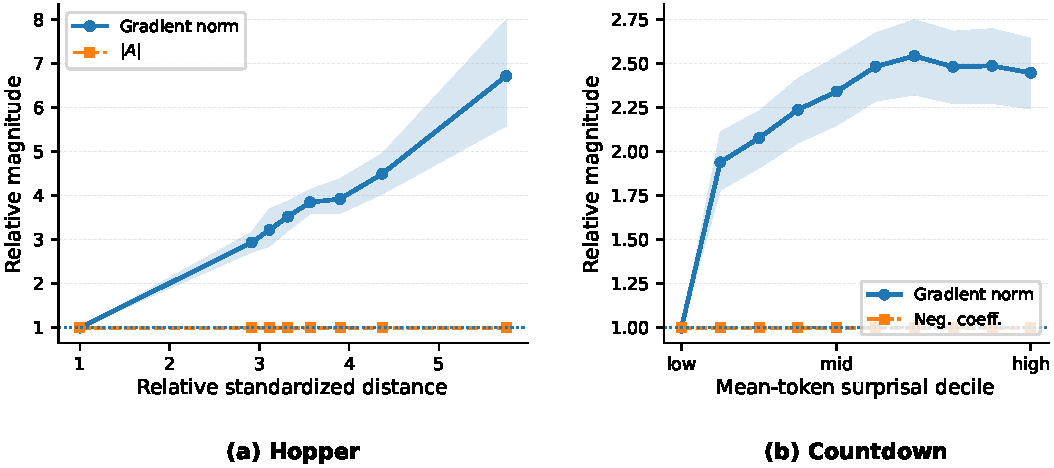
\includegraphics[
        width=\columnwidth
    ]{figures/figure1_external_gradient_bottom_labels.pdf}

    \caption{
        \textbf{External diagnostic of far-field negative influence.}
        \textbf{(a)} Hopper: relative full-parameter actor-gradient norm
        and matched absolute advantage as functions of relative standardized
        distance for transitions with negative learned-critic advantages.
        Values are normalized to the near-field reference within each seed.
        Lines report averages across 10 seeds, and shaded regions denote
        seed-level bootstrap 95\% confidence intervals.
        \textbf{(b)} Countdown: relative trainable-parameter gradient norm
        and fixed negative coefficient magnitude as functions of current-policy
        mean-token surprisal deciles among verifier-matched unsuccessful
        responses. Values are normalized to the lowest-surprisal decile, and
        shaded regions denote puzzle-level bootstrap 95\% confidence intervals.
    }
    \label{fig:external_far_field}
\end{figure}

We first examine two external settings that instantiate
learner-relative remoteness in different action spaces. Hopper provides
a continuous-control setting with a state-conditioned Gaussian policy,
where remoteness is measured by standardized distance from the current
policy. Countdown provides an autoregressive discrete setting, where
remoteness is measured by current-policy mean-token surprisal.

The diagnostic controls the sample-quality coefficient in each setting.
In Hopper, we compare negative-advantage transitions after matching their
absolute advantage magnitudes. In Countdown, we compare verifier-matched
unsuccessful responses while holding the negative coefficient magnitude
fixed. Thus, changes in gradient magnitude primarily reflect the
policy-score contribution rather than a larger negative coefficient.

Figure~\ref{fig:external_far_field} shows the same qualitative pattern
in both domains. In Hopper, the full-parameter actor-gradient norm grows
with standardized distance, while the matched absolute advantage remains
approximately flat. In Countdown, the trainable-parameter gradient norm
increases with mean-token surprisal, while the negative coefficient
remains fixed. These results provide external evidence that
learner-relative remoteness strengthens negative optimization influence
in both continuous learned-critic control and autoregressive policy
optimization.

The controlled experiments that follow isolate the source of this
amplification and test whether it causally propagates into policy drift
and collapse.




\subsection{Controlled Identification of the Causal Mechanism}
\label{sec:controlled_identification}

The external results show that far-field negative influence occurs in
realistic tasks, but sample quality, policy-relative remoteness, and
subsequent policy dynamics remain entangled. We therefore turn to C-U1
and D-U1, whose known task structure allows these factors to be varied
independently. We first isolate whether remoteness itself changes
negative influence and then test whether that influence causally
propagates into policy drift and collapse. Full constructions and
intervention protocols are provided in
Appendix~\ref{app:controlled_protocols}.

\subsubsection{Remoteness as an Independent Source of Negative Influence}
\label{sec:controlled_source}

\begin{figure}[t]
    \centering

    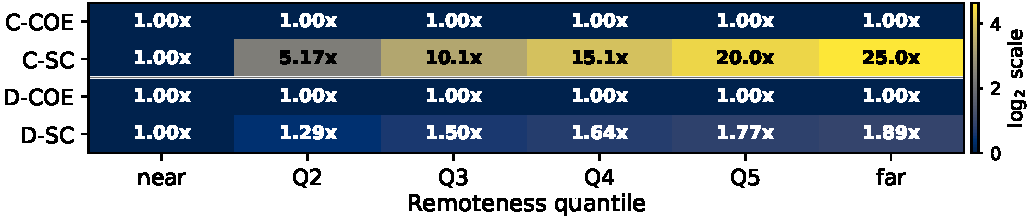
\includegraphics[
        width=0.92\columnwidth,
        trim={0pt 2pt 0pt 2pt},
        clip
    ]{figures/fig_6_3_1_source_heatmap.pdf}

    \vspace{0.35em}

    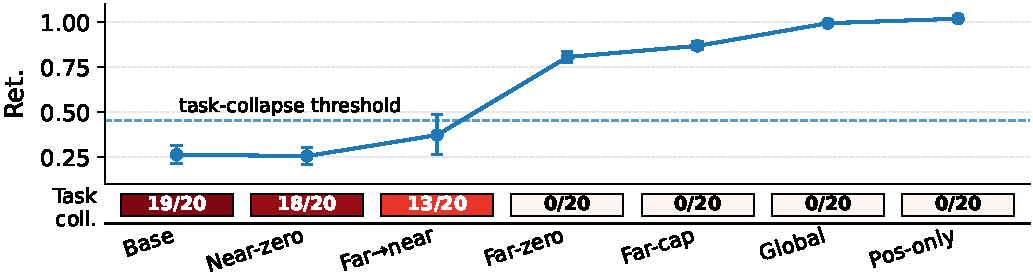
\includegraphics[
        width=0.92\columnwidth,
        trim={0pt 2pt 0pt 2pt},
        clip
    ]{figures/fig_6_3_2_rescue_plot.pdf}

    \vspace{-0.4em}

\caption{
    \textbf{Controlled source isolation and causal transmission.}
    \textbf{Top:} source-isolation factorization across
    learner-relative remoteness bins, normalized to the near bin.
    COE denotes coefficient magnitude and SC denotes policy-score
    response; C rows report the C-U1 continuous protocol, and D rows
    show the corresponding direct-softmax categorical reference.
    \textbf{Bottom:} C-U1 causal-intervention summary. Ret. denotes
    reward retention; points show 20-seed means with bootstrap
    confidence intervals, and Task coll. reports task-performance
    collapse counts.
}
    \label{fig:controlled_6_3}
\end{figure}

We first isolate whether learner-relative remoteness changes negative
influence independently of sample quality. In C-U1, negative actions are
placed on the same reward contour, giving them identical fixed
advantages but different standardized distances from the current
Gaussian policy. The categorical direct-softmax reference applies the
same factorization by fixing the negative coefficient while varying
current-policy surprisal.

The top panel of Figure~\ref{fig:controlled_6_3} separates the
coefficient term from the policy-score term. The coefficient magnitude
remains flat across remoteness bins, whereas the score response increases
with remoteness. Thus, the larger negative influence cannot be explained
by farther samples having larger advantages; it is generated by the
policy-score geometry itself. The manifestation differs across action
spaces: Gaussian policies exhibit amplitude amplification, while
categorical policies approach a bounded direct-logit score but continue
to suppress the selected action toward the simplex boundary. This
experiment identifies the source of the influence, not its downstream
causal effect.

\subsubsection{Causal Transmission into Drift and Collapse}
\label{sec:controlled_transmission}

We next test whether this far-field influence causally propagates into
instability. In the C-U1 intervention protocol, all branches share the
same data, fixed labels, initialization, optimizer, and training horizon,
and differ only in how near- and far-field negative updates are retained,
removed, capped, or globally rescaled.

The bottom panel of Figure~\ref{fig:controlled_6_3} shows a clear rescue
pattern. Removing near-field negative updates leaves performance collapse
largely unchanged, whereas removing or capping far-field updates restores
reward retention and eliminates task-performance collapse. Global
rescaling also rescues the run, supporting the interpretation that
abnormal negative-update magnitude is a mediator. In contrast,
transferring the far-field budget to near-field negatives gives only
partial recovery, showing that the rescue is not obtained by simply
preserving the same total negative-update budget.

These interventions identify far-field negative influence, rather than
negative feedback in general, as a causal transmission path to policy
instability in the controlled Gaussian environment. Task-performance
collapse is visualized in the figure; support or variance-boundary events
and NaN/Inf numerical failures are audited separately.

\subsection{From Useful Repulsion to DRPO Control}
\label{sec:repulsion_control}

The causal experiments show that the far-field tail must be controlled,
but they do not imply that all negative feedback should be removed.
The remaining question is how to preserve useful local repulsion while
attenuating harmful remote influence. We therefore separate two roles:
controlled taper-shape experiments identify which negative-weighting
profiles preserve local utility under known near/far structure, whereas
external experiments test whether the same control principle transfers
to realistic offline-control and autoregressive-generation settings. Positive-only learning
is stable but remains constrained by the observed positive support. C-U1
and D-U1 therefore place a hidden task optimum beyond the positive-only
target and construct local negative feedback whose repulsive direction
points toward that optimum, while additional remote negatives create
far-field pressure. This exposes a controlled transition from useful
local repulsion to harmful far-field dominance.

\subsubsection{Stable Extrapolation from Controlled Negative Feedback}
\label{sec:controlled_negative_strength}

\begin{figure}[t]
    \centering
    
\includegraphics[
        width=0.95\columnwidth
    ]{figures/fig_6_4_1_phase_transition.pdf}

    \vspace{-0.35em}
\caption{
    \textbf{Stable extrapolation from controlled negative feedback.}
    Increasing the effective negative strength $q/p$ first improves
    held-out-context reward beyond the positive-only ceiling, then causes
    over-extrapolation and task-performance collapse. Policy shift
    measures displacement from the positive-only target. The color strip
    reports task collapse, boundary events, and NaN/Inf failures
    separately.
}
    \label{fig:phase_transition_6_4_1}
\end{figure}

The causal interventions in Section~\ref{sec:controlled_transmission}
show that far-field negative influence must be controlled, but they do
not imply that all negative feedback should be removed. We therefore
sweep the effective negative strength relative to positive attraction,
denoted by $q/p$, while keeping the data, labels, initialization,
optimizer, and training horizon fixed; protocol and metric details are
given in Appendix~\ref{app:negative_strength_sweep}. The positive-only
setting is $q/p=0$.

Figure~\ref{fig:phase_transition_6_4_1} shows a non-monotone transition.
For small and moderate $q/p$, held-out-context reward rises above the
positive-only ceiling, showing that controlled negative feedback provides
useful repulsion beyond the positive-support solution. As $q/p$ grows
larger, policy shift continues to increase but reward declines,
indicating over-extrapolation rather than additional useful
generalization. At the largest strengths, task-performance collapse and
boundary events appear, while NaN/Inf failures are reported separately.

This strength sweep supplies the missing link between causal rescue and
tapered control: positive-only learning removes the harmful tail but also
removes the beneficial intermediate regime. Remoteness-aware control
should therefore preserve useful local repulsion while preventing the
far-field tail from dominating.


\begin{figure}[t]
\centering

\begin{minipage}[t]{0.68\columnwidth}
    \centering
    \vspace{0pt}
\textbf{(a) Controlled taper comparison}\\[0.05em]
    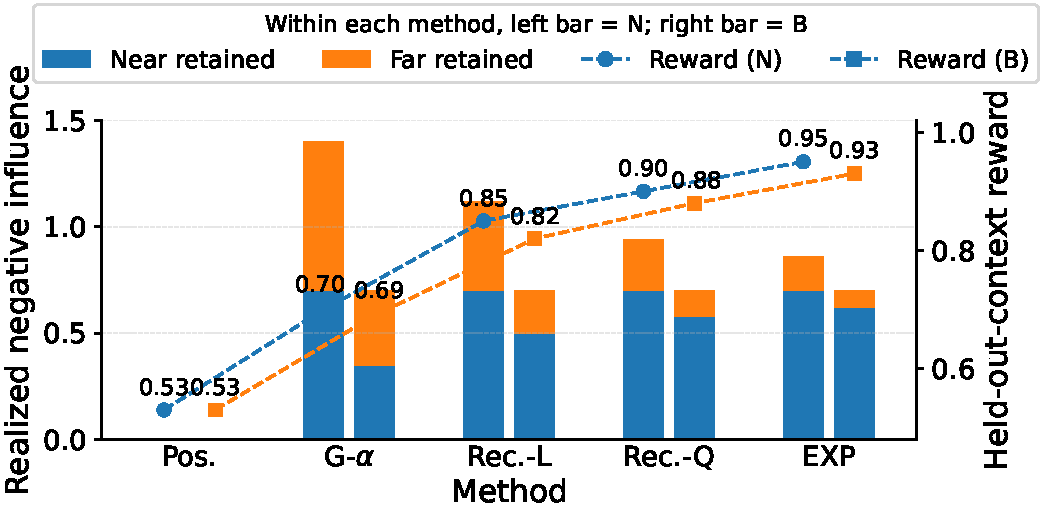
\includegraphics[
        width=\linewidth
    ]{figures/fig_6_4_2_leftfig_bigtext_legend_protocol.pdf}
\end{minipage}
\hfill
\begin{minipage}[t]{0.28\columnwidth}
    \centering
    \vspace{0pt}
    \textbf{(b) Transfer}\\[0.20em]    \scriptsize
    \setlength{\tabcolsep}{2.2pt}
    \renewcommand{\arraystretch}{0.92}
    \resizebox{\linewidth}{!}{
    \begin{tabular}{lcc}
    \toprule
    Method & Hop. & Cnt. \\
    \midrule
    Pos.        & \texttt{--} & \texttt{--} \\
    G-$\alpha$  & \texttt{--} & \texttt{--} \\
    Rec.-L      & \texttt{--} & \texttt{--} \\
    Rec.-Q      & \texttt{--} & \texttt{--} \\
    EXP         & \textbf{\texttt{--}} & \textbf{\texttt{--}} \\
    \bottomrule
    \end{tabular}
    }

    \vspace{0.25em}
    {\scriptsize
    Hop.: Hopper return.\\
    Cnt.: Countdown success.
    }
\end{minipage}

\vspace{-0.35em}
\caption{
\textbf{Controlled taper comparison and external transfer.}
\textbf{(a)} Matched operating-point comparison in the controlled
taper protocol. For each method, the left bar is the near-field-retention
matched operating point and the right bar is the aggregate-budget matched
operating point. Bars decompose retained negative influence into near-
and far-field components, and dashed traces report held-out-context reward.
\textbf{(b)} External validation summary on Hopper and Countdown. The
right panel reports only final task-level outcomes; operating-point and
matching details are shown in the controlled comparison.
}
\label{fig:taper_control_and_transfer}
\end{figure}

\subsubsection{Controlled Comparison of Taper Shapes}
\label{sec:controlled_tapers}

We compare positive-only learning, global negative scaling,
reciprocal-linear tapering, reciprocal-quadratic tapering, and
exponential tapering while changing only the negative weighting rule. Two
matched comparisons are used. Near-field-retention matching preserves
comparable local negative influence and isolates differences in far-field
decay, whereas aggregate-budget matching tests whether a selective taper
outperforms a global reduction with the same total negative-update
budget.

As shown in Figure~\ref{fig:taper_control_and_transfer}, exponential tapering
provides the strongest stability--utility trade-off under both matched
comparisons. Positive-only learning avoids far-field instability but
remains at the positive-support ceiling. Global scaling suppresses useful
near- and harmful far-field feedback indiscriminately. Reciprocal
tapering introduces remoteness-aware suppression, but its tail remains
heavier than the exponential rule. The exponential taper instead retains
near-field repulsion while rapidly suppressing the far-field tail,
yielding higher task performance and held-out-context generalization
than the matched alternatives.

\subsubsection{External Validation of Remoteness Tapering}
\label{sec:external_tapers}

We finally transfer the same control principle to Hopper and Countdown.
DRPO weights Hopper transitions by their standardized remoteness from
the current Gaussian policy and Countdown responses by their current
mean token surprisal. Within each task, all methods share the dataset,
initialization, labels, optimizer, and training budget. Because these
external tasks do not provide known counterfactual geometry or exact
near-field utility matching, they test transfer rather than repeat the
controlled causal identification.

The transfer panel in Figure~\ref{fig:taper_control_and_transfer} records
the same external validation targets without repeating the full controlled
taper ablation in the main text. Detailed protocol-matched comparisons are
reported with the task-level results and appendix materials. The controlled
stability--utility principle is therefore evaluated both in continuous
offline control and in autoregressive policy optimization.

\subsection{Overall Task Performance}
\label{sec:overall_performance}

Having established the mechanism and its transfer, we evaluate DRPO as
a complete policy-optimization method on D4RL locomotion and Countdown.
We compare it with published domain-specific baselines while keeping the
protocol-matched controls and alternative taper ablations in the controlled
comparison and appendix. We report normalized return for D4RL and verifier
success for Countdown, while task-performance failures, support or
variance-boundary events, and NaN/Inf numerical failures remain separate
outcomes.

% Required packages:
% \usepackage{booktabs}
% \usepackage{graphicx}

\subsubsection{D4RL Locomotion}
\label{sec:d4rl_performance}

We evaluate the nine D4RL Gym locomotion tasks formed by HalfCheetah,
Hopper, and Walker2d under the medium, medium-replay, and medium-expert
datasets. These datasets vary in behavior quality and coverage, with
medium-replay containing the broadest mixture of historical policies.
Table~\ref{tab:d4rl_performance} compares DRPO with published offline-RL
baselines under the D4RL evaluation protocol. The shared objectives and
taper functions are defined in Appendix~\ref{app:shared_methods};
D4RL-specific score provenance, uncertainty statistics, remoteness
construction, and implementation details are provided in
Appendix~\ref{app:d4rl_methods}.

\begin{table}[t]
\centering
\caption{Normalized returns on the D4RL-9 Gym locomotion benchmark.}
\label{tab:d4rl_performance}

\small
\setlength{\tabcolsep}{3.9pt}
\renewcommand{\arraystretch}{1.07}

\begin{tabular*}{\columnwidth}{@{\extracolsep{\fill}}lcccc}
\toprule
Dataset
&
CQL$^\dagger$
&
TD3+BC$^\dagger$
&
IQL$^\dagger$
&
\textbf{DRPO}
\\
\midrule

halfcheetah-medium
& 44.0 & \textbf{48.3} & \underline{47.4} & 47.3 \\
hopper-medium
& 58.5 & 59.3 & \textbf{66.3} & \underline{63.3} \\
walker2d-medium
& 72.5 & \underline{83.7} & 78.3 & \textbf{85.5} \\

\midrule

halfcheetah-replay
& \textbf{45.5} & \underline{44.6} & 44.2 & 43.3 \\
hopper-replay
& \underline{95.0} & 60.9 & 94.7 & \textbf{95.8} \\
walker2d-replay
& 77.2 & \textbf{81.8} & 73.9 & \underline{78.1} \\

\midrule

halfcheetah-expert
& \textbf{91.6} & 90.7 & 86.7 & \underline{91.1} \\
hopper-expert
& \textbf{105.4} & 98.0 & 91.5 & \underline{101.8} \\
walker2d-expert
& 108.8 & \underline{110.1} & 109.6 & \textbf{110.4} \\

\midrule

\textit{D4RL-9 total}
& \textit{\underline{698.5}}
& \textit{677.4}
& \textit{692.4}
& \textbf{\textit{716.6}}
\\

\bottomrule
\end{tabular*}

\vspace{2pt}

\begin{minipage}{\columnwidth}
\small
\textit{Note.}
Dataset names are shortened for compactness: ``replay'' denotes
``medium-replay'', ``expert'' denotes ``medium-expert'', and the D4RL
``-v2'' suffix is omitted. Results marked by $\dagger$ are reported by
prior work rather than protocol-matched reruns. Rows report task-level
normalized returns, and \textit{D4RL-9 total} sums the nine task means.
Bold and underlined values denote the best and second-best results among
the methods shown in this table. DRPO results are averaged over 10 runs;
standard deviations and seed-level results are reported in
Appendix~\ref{app:d4rl_methods}.
\end{minipage}

\end{table}

DRPO achieves the highest aggregate performance across D4RL-9, with a
total normalized return of 716.6. Its advantage is largest on the
medium-replay tasks, where broader behavioral coverage creates stronger
far-field pressure, while remaining competitive on the medium and
medium-expert datasets. These results indicate that selective
remoteness-aware attenuation remains effective in a standard
learned-critic offline-control benchmark.

\subsubsection{Countdown}
\label{sec:countdown_performance}

We evaluate DRPO on held-out Countdown puzzles, where a response is
successful only if it forms a valid arithmetic expression that uses the
provided numbers and reaches the target value. Greedy verifier success
is the primary metric, while pass@$k$ measures sampling-level solution
coverage and valid-expression rate distinguishes reasoning failure from
formatting or execution failure.

All compared policy-optimization methods start from the same SFT
checkpoint and use the same frozen response bank, training budget,
validation split, and test puzzles. We compare DRPO with
AsymRE~\citep{arnal2025asymmetric} and
TOPR~\citep{leroux2025tapered} as off-policy baselines.
The shared objectives and taper functions are defined in
Appendix~\ref{app:shared_methods}; Countdown-specific baseline
implementations, response-bank construction, checkpoint selection, and
evaluation details are provided in
Appendix~\ref{app:countdown_methods}.

\begin{table}[t]
\centering
\caption{Performance on held-out Countdown puzzles.}
\label{tab:countdown_performance}

\small
\renewcommand{\arraystretch}{1.10}
\setlength{\tabcolsep}{5.0pt}

\begin{tabular*}{\columnwidth}{@{\extracolsep{\fill}}lccc}
\toprule
Metric
&
AsymRE
&
TOPR
&
\textbf{DRPO}
\\
\midrule

Greedy success (\%)
& --
& --
& --
\\

Pass@$k$ (\%)
& --
& --
& --
\\

Valid expression (\%)
& --
& --
& --
\\

\bottomrule
\end{tabular*}

\vspace{2pt}

\begin{minipage}{\columnwidth}
\small
\textit{Note.}
All methods use the same SFT checkpoint, frozen response bank,
validation split, test puzzles, and training budget. A dash denotes a
result pending the formal run.
\end{minipage}

\end{table}

DRPO achieves the highest greedy verifier success among the methods
shown in Table~\ref{tab:countdown_performance}, reaching \emph{[TBD]}.
It improves over AsymRE and TOPR by \emph{[TBD]} and \emph{[TBD]},
respectively. DRPO also obtains the highest pass@$k$ while maintaining
a valid-expression rate of \emph{[TBD]}, showing that the improvement
comes from solving more puzzles rather than relaxing output validity.

\section{Conclusion}

This work reframes negative feedback in off-policy policy optimization
as a controlled resource rather than a signal to be uniformly kept or
removed. Its value depends on where a historical action lies relative to
the current learner: nearby failures can shape useful decision
boundaries, while remote failures can acquire disproportionate influence
and destabilize optimization. DRPO operationalizes this view by
attenuating negative influence according to learner-relative remoteness,
preserving locally informative repulsion while limiting the far-field
tail. The broader lesson is that stable offline and off-policy policy
optimization should control the geometry of reused feedback, not merely
its sign or magnitude.


% Acknowledgements should only appear in the accepted version.


% In the unusual situation where you want a paper to appear in the
% references without citing it in the main text, use \nocite
\nocite{langley00}

\bibliography{references}
\bibliographystyle{icml2026}

%%%%%%%%%%%%%%%%%%%%%%%%%%%%%%%%%%%%%%%%%%%%%%%%%%%%%%%%%%%%%%%%%%%%%%%%%%%%%%%
%%%%%%%%%%%%%%%%%%%%%%%%%%%%%%%%%%%%%%%%%%%%%%%%%%%%%%%%%%%%%%%%%%%%%%%%%%%%%%%
% APPENDIX
%%%%%%%%%%%%%%%%%%%%%%%%%%%%%%%%%%%%%%%%%%%%%%%%%%%%%%%%%%%%%%%%%%%%%%%%%%%%%%%
%%%%%%%%%%%%%%%%%%%%%%%%%%%%%%%%%%%%%%%%%%%%%%%%%%%%%%%%%%%%%%%%%%%%%%%%%%%%%%%
\newpage
\appendix
\onecolumn
\section{Proofs for the Theoretical Results}
\label{app:theory_proofs}
\subsection{Proof of Proposition~\ref{prop:distance_strength}}
\label{app:distance_strength}

\begin{proof}
Let $\delta=a-\mu$. For a Gaussian policy with fixed covariance
$\Sigma$,
\begin{equation}
    D_\mu(a)-C_\Sigma
    =
    \frac{1}{2}
    \delta^\top\Sigma^{-1}\delta.
    \label{eq:proof_gaussian_remoteness}
\end{equation}
The mean score function is
\begin{equation}
    \mathbf{s}_\mu(a)
    =
    \nabla_\mu\log\pi_\mu(a)
    =
    \Sigma^{-1}\delta,
\end{equation}
and hence
\begin{equation}
    R_\mu(a)
    =
    \left\|\mathbf{s}_\mu(a)\right\|_2^2
    =
    \delta^\top\Sigma^{-2}\delta.
    \label{eq:proof_gaussian_score_norm}
\end{equation}
Let $x=\Sigma^{-1/2}\delta$. Then
\begin{equation}
    D_\mu(a)-C_\Sigma
    =
    \frac{1}{2}\|x\|_2^2,
    \qquad
    R_\mu(a)
    =
    x^\top\Sigma^{-1}x.
\end{equation}
Applying the Rayleigh quotient bounds gives
\begin{equation}
\begin{aligned}
    R_\mu(a)
    &\geq
    2\lambda_{\min}(\Sigma^{-1})
    \bigl(D_\mu(a)-C_\Sigma\bigr), \\
    R_\mu(a)
    &\leq
    2\lambda_{\max}(\Sigma^{-1})
    \bigl(D_\mu(a)-C_\Sigma\bigr).
\end{aligned}
\end{equation}

If $\delta=rv$ for a fixed direction $v\neq0$, then
\begin{equation}
\begin{aligned}
    D_\mu(a)-C_\Sigma
    &=
    \frac{r^2}{2}
    v^\top\Sigma^{-1}v, \\
    R_\mu(a)
    &=
    r^2v^\top\Sigma^{-2}v.
\end{aligned}
\end{equation}
Eliminating $r^2$ proves
Equation~\eqref{eq:gaussian_directional_response}.
For the categorical policy, let
\begin{equation}
    p
    =
    \pi_z(a)
    =
    e^{-D_z(a)}.
\end{equation}
The score function with respect to the logits is
\begin{equation}
    \mathbf{s}_z(a)
    =
    \nabla_z\log\pi_z(a)
    =
    e_a-\pi_z.
\end{equation}
Its selected-action component is therefore
\begin{equation}
    \left|
        \frac{\partial}{\partial z_a}
        \log\pi_z(a)
    \right|
    =
    1-p
    =
    1-e^{-D_z(a)},
\end{equation}
which proves
Equation~\eqref{eq:categorical_selected_response}.
Since $1-e^{-D}$ is strictly increasing for $D\geq0$ and
converges to $1$ as $D\rightarrow\infty$, the selected-logit
response increases with surprisal but remains bounded.

For completeness, the squared norm of the full categorical
score function is
\begin{equation}
\begin{aligned}
    R_z(a)
    &=
    \left\|
        e_a-\pi_z
    \right\|_2^2 \\
    &=
    (1-p)^2
    +
    \sum_{j\neq a}\pi_z(j)^2.
\end{aligned}
\end{equation}
Because the non-selected probabilities sum to $1-p$,
the Cauchy--Schwarz inequality gives
\begin{equation}
    \sum_{j\neq a}\pi_z(j)^2
    \geq
    \frac{(1-p)^2}{K-1}.
\end{equation}
The same sum is at most $(1-p)^2$. Hence,
\begin{equation}
\begin{aligned}
    \frac{K}{K-1}(1-p)^2
    &\leq
    R_z(a) \\
    &\leq
    2(1-p)^2.
\end{aligned}
\end{equation}
Substituting $p=e^{-D_z(a)}$ completes the categorical
part of the proof.
\end{proof}
\subsection{Proof of Theorem~\ref{thm:reuse_dynamics}}
\label{app:reuse_dynamics}

\begin{proof}
Let
\[
    f(u)=D(u),
    \qquad
    g_t=\nabla f(u_t),
    \qquad
    R_t=\|g_t\|_2^2.
\]

We first consider a negative coefficient
$\widehat{A}=-c$ with $c>0$. Defining
$\alpha=\eta c$, the update becomes
\[
    u_{t+1}
    =
    u_t+\alpha g_t.
\]
By convexity of $f$,
\begin{align}
    f(u_{t+1})
    &\geq
    f(u_t)
    +
    g_t^\top(u_{t+1}-u_t) \\
    &=
    f(u_t)+\alpha\|g_t\|_2^2.
\end{align}
Hence,
\[
    D_{t+1}
    \geq
    D_t+\eta|\widehat{A}|R_t.
\]

The gradient of a differentiable convex function is monotone, so
\[
    \bigl(g_{t+1}-g_t\bigr)^\top
    \bigl(u_{t+1}-u_t\bigr)
    \geq0.
\]
Using $u_{t+1}-u_t=\alpha g_t$ gives
\[
    g_{t+1}^\top g_t
    \geq
    \|g_t\|_2^2.
\]
By the Cauchy--Schwarz inequality,
\[
    \|g_{t+1}\|_2\|g_t\|_2
    \geq
    g_{t+1}^\top g_t
    \geq
    \|g_t\|_2^2.
\]
Whenever $\|g_t\|_2>0$, division by $\|g_t\|_2$ yields
\[
    \|g_{t+1}\|_2
    \geq
    \|g_t\|_2,
\]
and therefore $R_{t+1}\geq R_t$. The same result is immediate when
$R_t=0$. The inequality is strict whenever the gradient changes
nontrivially along a direction of positive curvature.

We next consider a positive coefficient
$\widehat{A}=c$ with $c>0$. Let
$\alpha=\eta c$, so that
\[
    u_{t+1}
    =
    u_t-\alpha g_t.
\]
Because $f$ has an $L$-Lipschitz gradient, the descent lemma gives
\begin{align}
    f(u_{t+1})
    &\leq
    f(u_t)
    -
    \alpha\|g_t\|_2^2
    +
    \frac{L\alpha^2}{2}\|g_t\|_2^2 \\
    &=
    f(u_t)
    -
    \alpha
    \left(
        1-\frac{L\alpha}{2}
    \right)
    \|g_t\|_2^2.
\end{align}
If $\alpha\leq1/L$, then
\[
    D_{t+1}
    \leq
    D_t-\frac{\alpha}{2}R_t
    =
    D_t-\frac{\eta\widehat{A}}{2}R_t.
\]

It remains to show that the score-function norm does not increase.
For a convex function with an $L$-Lipschitz gradient, the gradient is
$1/L$-cocoercive:
\[
    \bigl(g_t-g_{t+1}\bigr)^\top
    \bigl(u_t-u_{t+1}\bigr)
    \geq
    \frac{1}{L}
    \|g_t-g_{t+1}\|_2^2.
\]
Let $d=g_{t+1}-g_t$. Since
$u_t-u_{t+1}=\alpha g_t$, this implies
\[
    d^\top g_t
    \leq
    -
    \frac{1}{\alpha L}
    \|d\|_2^2.
\]
Consequently,
\begin{align}
    \|g_{t+1}\|_2^2
    &=
    \|g_t+d\|_2^2 \\
    &=
    \|g_t\|_2^2
    +
    2d^\top g_t
    +
    \|d\|_2^2 \\
    &\leq
    \|g_t\|_2^2
    +
    \left(
        1-\frac{2}{\alpha L}
    \right)
    \|d\|_2^2.
\end{align}
Because $\alpha L\leq1$, the final coefficient is nonpositive, and hence
\[
    R_{t+1}
    =
    \|g_{t+1}\|_2^2
    \leq
    \|g_t\|_2^2
    =
    R_t.
\]
This proves both claims.
\end{proof}

\subsection{Derivation and Proof of
Theorem~\ref{thm:aggregate_equilibrium}}
\label{app:aggregate_equilibrium}

For the exponential-family policy in
Equation~\eqref{eq:exponential_family_policy}, define the signed
population objective
\begin{equation}
    \mathcal{L}(\eta)
    =
    \mathbb{E}_{a\sim\nu}
    \left[
        \widehat{A}(a)
        \log\pi_\eta(a)
    \right].
    \label{eq:app_signed_objective}
\end{equation}
Using
$\widehat{A}=\widehat{A}^{+}-\widehat{A}^{-}$
and Equation~\eqref{eq:aggregate_statistics}, we obtain
\begin{equation}
\begin{aligned}
    \mathcal{L}(\eta)
    &=
    \left(
        p\mathbf{m}_{+}
        -
        q\mathbf{m}_{-}
    \right)^\top\eta \\
    &\quad
    -
    (p-q)\psi(\eta)
    +
    C,
\end{aligned}
\label{eq:app_signed_objective_expansion}
\end{equation}
where
\begin{equation}
    C
    =
    \mathbb{E}_{\nu}
    \left[
        \widehat{A}(a)\log h(a)
    \right]
\end{equation}
is independent of $\eta$. Therefore,
\begin{equation}
    \nabla\mathcal{L}(\eta)
    =
    p\mathbf{m}_{+}
    -
    q\mathbf{m}_{-}
    -
    (p-q)\nabla\psi(\eta)
    =
    \mathbf{F}(\eta),
    \label{eq:app_aggregate_field}
\end{equation}
and
\begin{equation}
    \nabla^2\mathcal{L}(\eta)
    =
    -(p-q)\nabla^2\psi(\eta).
    \label{eq:app_signed_hessian}
\end{equation}
Because the exponential family is regular and minimal,
$\nabla^2\psi(\eta)\succ0$ throughout $\mathcal{H}$.

\begin{proof}
\medskip
\noindent\textbf{Positive-dominant regime.}
Suppose $p>q$. A finite equilibrium must satisfy
\begin{equation}
    \mathbf{F}(\eta^{\star})
    =
    \mathbf{0},
\end{equation}
which is equivalent to
\begin{equation}
    \nabla\psi(\eta^{\star})
    =
    \frac{
        p\mathbf{m}_{+}
        -
        q\mathbf{m}_{-}
    }{
        p-q
    }
    =
    \mathbf{m}^{\star}.
    \label{eq:app_equilibrium_condition}
\end{equation}
If $\mathbf{m}^{\star}\in\mathcal{M}$, existence follows because
$\nabla\psi$ maps $\mathcal{H}$ onto $\mathcal{M}$, and uniqueness
follows because this map is one-to-one.

Since $p-q>0$, Equation~\eqref{eq:app_signed_hessian} gives
\begin{equation}
    \nabla^2\mathcal{L}(\eta)
    \prec
    0.
\end{equation}
Thus, $\mathcal{L}$ is strictly concave, and $\eta^{\star}$ is its
unique global maximizer.

For the continuous dynamics, the field Jacobian at the equilibrium is
\begin{equation}
    J_{\mathbf{F}}(\eta^{\star})
    =
    -(p-q)
    \nabla^2\psi(\eta^{\star})
    \prec
    0.
    \label{eq:app_continuous_jacobian}
\end{equation}
All eigenvalues are strictly negative, so $\eta^{\star}$ is locally
asymptotically stable.

For the discrete update, the local update Jacobian is
\begin{equation}
    J_{\mathrm{disc}}(\eta^{\star})
    =
    I
    -
    \alpha(p-q)
    \nabla^2\psi(\eta^{\star}).
    \label{eq:app_discrete_jacobian}
\end{equation}
Let $\lambda_i>0$ denote the eigenvalues of
$\nabla^2\psi(\eta^{\star})$. The corresponding eigenvalues of
$J_{\mathrm{disc}}(\eta^{\star})$ are
\begin{equation}
    1
    -
    \alpha(p-q)\lambda_i.
\end{equation}
Their magnitudes are strictly smaller than one whenever
\begin{equation}
    0
    <
    \alpha
    <
    \frac{
        2
    }{
        (p-q)
        \lambda_{\max}
        \left(
            \nabla^2\psi(\eta^{\star})
        \right)
    }.
    \label{eq:app_discrete_stepsize}
\end{equation}
This proves local discrete-time stability for sufficiently small
$\alpha$.

When $q>0$, subtracting $\mathbf{m}_{+}$ from the signed target yields
\begin{equation}
\begin{aligned}
    \mathbf{m}^{\star}
    -
    \mathbf{m}_{+}
    &=
    \frac{
        p\mathbf{m}_{+}
        -
        q\mathbf{m}_{-}
    }{
        p-q
    }
    -
    \mathbf{m}_{+} \\
    &=
    \frac{q}{p-q}
    \left(
        \mathbf{m}_{+}
        -
        \mathbf{m}_{-}
    \right).
\end{aligned}
\end{equation}
This proves
Equation~\eqref{eq:stable_extrapolation_identity}.
If $q=0$, the signed target reduces directly to
$\mathbf{m}_{+}$.

If $\mathbf{m}^{\star}\notin\mathcal{M}$, no finite
$\eta^{\star}\in\mathcal{H}$ can satisfy
Equation~\eqref{eq:app_equilibrium_condition}, and hence no finite
equilibrium exists.

Now consider a sequence
$\mathbf{m}^{\star}_n\in\mathcal{M}$
that approaches the boundary of $\mathcal{M}$, and define
\begin{equation}
    \eta^{\star}_n
    =
    (\nabla\psi)^{-1}
    \left(
        \mathbf{m}^{\star}_n
    \right).
\end{equation}
Suppose, for contradiction, that
$\{\eta^{\star}_n\}$ remains in a compact subset of $\mathcal{H}$.
Then some subsequence converges to a finite
$\bar{\eta}\in\mathcal{H}$. By continuity,
\begin{equation}
    \mathbf{m}^{\star}_n
    =
    \nabla\psi(\eta^{\star}_n)
    \longrightarrow
    \nabla\psi(\bar{\eta})
    \in
    \mathcal{M},
\end{equation}
contradicting convergence to the boundary. Hence, the corresponding
natural parameters must leave every compact subset of $\mathcal{H}$.

\medskip
\noindent\textbf{Critical regime.}
Suppose $p=q$. Equation~\eqref{eq:app_aggregate_field} reduces to
\begin{equation}
    \mathbf{F}(\eta)
    =
    p
    \left(
        \mathbf{m}_{+}
        -
        \mathbf{m}_{-}
    \right),
    \label{eq:app_critical_field}
\end{equation}
which is independent of $\eta$.

If $\mathbf{m}_{+}\neq\mathbf{m}_{-}$, the continuous trajectory is
\begin{equation}
    \eta(t)
    =
    \eta(0)
    +
    tp
    \left(
        \mathbf{m}_{+}
        -
        \mathbf{m}_{-}
    \right),
    \label{eq:app_critical_continuous}
\end{equation}
and the discrete trajectory is
\begin{equation}
    \eta_t
    =
    \eta_0
    +
    t\alpha p
    \left(
        \mathbf{m}_{+}
        -
        \mathbf{m}_{-}
    \right).
    \label{eq:app_critical_discrete}
\end{equation}
Both exhibit persistent linear drift and admit no finite equilibrium.

If $\mathbf{m}_{+}=\mathbf{m}_{-}$, then
$\mathbf{F}(\eta)=\mathbf{0}$ for every $\eta$. Every point is
stationary, but a perturbed trajectory remains at the perturbed point
rather than returning to the original one. Hence, no point is an
isolated locally asymptotically stable equilibrium.

\medskip
\noindent\textbf{Negative-dominant regime.}
Suppose $p<q$. Equation~\eqref{eq:app_signed_hessian} gives
\begin{equation}
    \nabla^2\mathcal{L}(\eta)
    =
    (q-p)
    \nabla^2\psi(\eta)
    \succ
    0.
\end{equation}
Thus, $\mathcal{L}$ is strictly convex.

If a finite stationary point $\eta^{\star}$ exists, the continuous
field Jacobian is
\begin{equation}
    J_{\mathbf{F}}(\eta^{\star})
    =
    (q-p)
    \nabla^2\psi(\eta^{\star})
    \succ
    0.
    \label{eq:app_negative_continuous_jacobian}
\end{equation}
All eigenvalues are positive, so the stationary point is repelling and
therefore unstable.

For the discrete update, the local Jacobian is
\begin{equation}
    J_{\mathrm{disc}}(\eta^{\star})
    =
    I
    +
    \alpha(q-p)
    \nabla^2\psi(\eta^{\star}).
    \label{eq:app_negative_discrete_jacobian}
\end{equation}
Its eigenvalues are
\begin{equation}
    1
    +
    \alpha(q-p)\lambda_i
    >
    1
\end{equation}
for every $\alpha>0$ and every
$\lambda_i>0$. Therefore, any finite stationary point is unstable under
the discrete dynamics as well. If no stationary point exists, there is
trivially no finite stable equilibrium.

The three regimes establish
Theorem~\ref{thm:aggregate_equilibrium}.
\end{proof}

\subsection{Proof of
Theorem~\ref{thm:policy_family_manifestations}}
\label{app:policy_family_manifestations}

\begin{proof}
Let
\begin{equation}
    r
    =
    q-p
    >
    0.
\end{equation}

\medskip
\noindent\textbf{Gaussian policy.}
For a Gaussian policy with fixed covariance,
\begin{equation}
    \nabla_{\mu}
    \log\pi_{\mu}(a)
    =
    \Sigma^{-1}(a-\mu).
    \label{eq:app_gaussian_mean_score}
\end{equation}
The aggregate mean field is therefore
\begin{equation}
\begin{aligned}
    \mathbf{F}_{\mu}(\mu)
    &=
    \mathbb{E}_{\nu}
    \left[
        \widehat{A}(a)
        \Sigma^{-1}(a-\mu)
    \right] \\
    &=
    \Sigma^{-1}
    \left[
        p\mu_{+}
        -
        q\mu_{-}
        -
        (p-q)\mu
    \right].
\end{aligned}
\label{eq:app_gaussian_aggregate_field}
\end{equation}
Because $p-q=-r$ and
\begin{equation}
    \mu^{\dagger}
    =
    \frac{
        q\mu_{-}
        -
        p\mu_{+}
    }{
        r
    },
\end{equation}
Equation~\eqref{eq:app_gaussian_aggregate_field} becomes
\begin{equation}
    \mathbf{F}_{\mu}(\mu)
    =
    r\Sigma^{-1}
    \left(
        \mu-\mu^{\dagger}
    \right).
\end{equation}

For the continuous dynamics, define
\begin{equation}
    \delta(t)
    =
    \mu(t)-\mu^{\dagger}.
\end{equation}
Then
\begin{equation}
    \dot{\delta}(t)
    =
    r\Sigma^{-1}\delta(t),
\end{equation}
and hence
\begin{equation}
    \delta(t)
    =
    \exp
    \left(
        r\Sigma^{-1}t
    \right)
    \delta(0).
    \label{eq:app_gaussian_continuous_solution}
\end{equation}
Since $\Sigma^{-1}\succ0$,
\begin{equation}
    \left\|
        \delta(t)
    \right\|_2
    \geq
    \exp
    \left(
        r\lambda_{\min}
        \left(
            \Sigma^{-1}
        \right)t
    \right)
    \left\|
        \delta(0)
    \right\|_2.
    \label{eq:app_gaussian_continuous_growth}
\end{equation}
Therefore, unless
$\delta(0)=0$, the distance from the stationary point grows
exponentially and
$\|\mu(t)\|_2\rightarrow\infty$.

For the discrete update,
\begin{equation}
    \mu_{t+1}
    =
    \mu_t
    +
    \alpha
    \mathbf{F}_{\mu}(\mu_t),
\end{equation}
so
\begin{equation}
    \delta_{t+1}
    =
    \left(
        I
        +
        \alpha r\Sigma^{-1}
    \right)
    \delta_t.
\end{equation}
Iterating gives
\begin{equation}
    \delta_t
    =
    \left(
        I
        +
        \alpha r\Sigma^{-1}
    \right)^t
    \delta_0.
    \label{eq:app_gaussian_discrete_solution}
\end{equation}
All eigenvalues of the update matrix are strictly larger than one.
Consequently,
\begin{equation}
    \left\|
        \delta_t
    \right\|_2
    \geq
    \left[
        1
        +
        \alpha r
        \lambda_{\min}
        \left(
            \Sigma^{-1}
        \right)
    \right]^t
    \left\|
        \delta_0
    \right\|_2.
    \label{eq:app_gaussian_discrete_growth}
\end{equation}
Thus, every nonstationary discrete trajectory also diverges.

For any fixed historical action $a$,
\begin{equation}
\begin{aligned}
    \left\|
        \nabla_{\mu}
        \log\pi_{\mu}(a)
    \right\|_2
    &=
    \left\|
        \Sigma^{-1}(a-\mu)
    \right\|_2 \\
    &\geq
    \lambda_{\min}
    \left(
        \Sigma^{-1}
    \right)
    \left\|
        a-\mu
    \right\|_2.
\end{aligned}
\label{eq:app_gaussian_score_lower_bound}
\end{equation}
Since $\|\mu\|_2\rightarrow\infty$ while $a$ is fixed,
$\|a-\mu\|_2\rightarrow\infty$.
Equation~\eqref{eq:app_gaussian_score_lower_bound} therefore proves
Equation~\eqref{eq:gaussian_unbounded_score}.

\medskip
\noindent\textbf{Categorical policy.}
Let there be $K\geq2$ actions and write
\begin{equation}
    \pi_z
    =
    \operatorname{softmax}(z).
\end{equation}
Because adding a constant to every logit does not change the policy, we
work on the gauge-fixed subspace
\begin{equation}
    \mathcal{H}_0
    =
    \left\{
        z\in\mathbb{R}^{K}
        :
        \mathbf{1}^{\top}z=0
    \right\}.
    \label{eq:app_categorical_gauge}
\end{equation}

Let $\rho_{+}$ and $\rho_{-}$ denote the normalized positive and negative
weighted action distributions, and define
\begin{equation}
    b
    =
    p\rho_{+}
    -
    q\rho_{-}.
\end{equation}
The signed categorical objective can be written as
\begin{equation}
    \mathcal{L}(z)
    =
    b^{\top}z
    +
    r
    \log
    \left(
        \sum_{j=1}^{K}
        e^{z_j}
    \right)
    +
    C,
    \label{eq:app_categorical_objective}
\end{equation}
because $p-q=-r$. Its gradient and Hessian are
\begin{equation}
    \nabla\mathcal{L}(z)
    =
    b+r\pi_z
\end{equation}
and
\begin{equation}
    \nabla^2\mathcal{L}(z)
    =
    r
    \left[
        \operatorname{Diag}(\pi_z)
        -
        \pi_z\pi_z^{\top}
    \right].
    \label{eq:app_categorical_hessian}
\end{equation}
For every nonzero
$v\in\mathcal{H}_0$,
\begin{equation}
\begin{aligned}
    v^{\top}
    \nabla^2\mathcal{L}(z)
    v
    &=
    r
    \operatorname{Var}_{A\sim\pi_z}
    \left[
        v_A
    \right] \\
    &>
    0,
\end{aligned}
\end{equation}
because every softmax probability is positive and a nonzero vector in
$\mathcal{H}_0$ cannot be constant. Hence,
$\mathcal{L}$ is strictly convex on $\mathcal{H}_0$ and has at most one
finite stationary point.

Consider first the continuous gradient flow
\begin{equation}
    \dot{z}
    =
    \nabla\mathcal{L}(z).
\end{equation}
Along every trajectory,
\begin{equation}
    \frac{d}{dt}
    \mathcal{L}(z(t))
    =
    \left\|
        \nabla\mathcal{L}(z(t))
    \right\|_2^2
    \geq
    0.
    \label{eq:app_categorical_objective_growth}
\end{equation}
Suppose a nonstationary trajectory were bounded. Its closure would be
compact, so $\mathcal{L}$ would remain bounded above. Integrating
Equation~\eqref{eq:app_categorical_objective_growth} would then give
\begin{equation}
    \int_0^\infty
    \left\|
        \nabla\mathcal{L}(z(t))
    \right\|_2^2
    dt
    <
    \infty.
\end{equation}
Since the gradient is Lipschitz on the compact trajectory closure, the
standard gradient-flow argument implies
\begin{equation}
    \nabla\mathcal{L}(z(t))
    \longrightarrow
    0.
\end{equation}
Any accumulation point would therefore be a stationary point.

If no finite stationary point exists, this is an immediate
contradiction. If a stationary point $z^{\dagger}$ exists, strict
convexity gives, for every $z\neq z^{\dagger}$,
\begin{equation}
    (z-z^{\dagger})^{\top}
    \left[
        \nabla\mathcal{L}(z)
        -
        \nabla\mathcal{L}(z^{\dagger})
    \right]
    >
    0.
\end{equation}
Since
$\nabla\mathcal{L}(z^{\dagger})=0$,
\begin{equation}
    \frac{d}{dt}
    \frac{1}{2}
    \left\|
        z(t)-z^{\dagger}
    \right\|_2^2
    >
    0
\end{equation}
along every nonstationary trajectory. Such a trajectory cannot have a
subsequence converging to $z^{\dagger}$. Hence, the only bounded
continuous trajectory is the stationary one itself.

For the discrete update
\begin{equation}
    z_{t+1}
    =
    z_t
    +
    \alpha
    \nabla\mathcal{L}(z_t),
    \qquad
    \alpha>0,
\end{equation}
convexity gives
\begin{equation}
\begin{aligned}
    \mathcal{L}(z_{t+1})
    &\geq
    \mathcal{L}(z_t)
    +
    \nabla\mathcal{L}(z_t)^{\top}
    (z_{t+1}-z_t) \\
    &=
    \mathcal{L}(z_t)
    +
    \alpha
    \left\|
        \nabla\mathcal{L}(z_t)
    \right\|_2^2.
\end{aligned}
\label{eq:app_categorical_discrete_growth}
\end{equation}
If the trajectory were bounded,
Equation~\eqref{eq:app_categorical_discrete_growth} would imply
\begin{equation}
    \nabla\mathcal{L}(z_t)
    \longrightarrow
    0.
\end{equation}
A convergent subsequence would therefore approach a finite stationary
point. If no such point exists, this is impossible. If the unique
stationary point $z^{\dagger}$ exists, then for
$z_t\neq z^{\dagger}$,
\begin{equation}
\begin{aligned}
    \left\|
        z_{t+1}-z^{\dagger}
    \right\|_2^2
    &=
    \left\|
        z_t-z^{\dagger}
    \right\|_2^2 \\
    &\quad
    +
    2\alpha
    (z_t-z^{\dagger})^{\top}
    \nabla\mathcal{L}(z_t) \\
    &\quad
    +
    \alpha^2
    \left\|
        \nabla\mathcal{L}(z_t)
    \right\|_2^2 \\
    &>
    \left\|
        z_t-z^{\dagger}
    \right\|_2^2.
\end{aligned}
\end{equation}
The trajectory therefore cannot have a subsequence converging to
$z^{\dagger}$. Thus, every nonstationary discrete trajectory leaves
every compact subset of $\mathcal{H}_0$.

To relate logit divergence to the probability boundary, note that on
$\mathcal{H}_0$ the inverse softmax representation is
\begin{equation}
    z_i
    =
    \log\pi_z(i)
    -
    \frac{1}{K}
    \sum_{j=1}^{K}
    \log\pi_z(j).
    \label{eq:app_inverse_softmax}
\end{equation}
If the probabilities remained in a compact subset of the simplex
interior, all coordinates would be bounded below by some
$\varepsilon>0$, and
Equation~\eqref{eq:app_inverse_softmax} would imply bounded logits.
Therefore, an unbounded gauge-fixed logit trajectory must contain a
subsequence along which at least one action probability approaches zero.

Finally, for every action $a$,
\begin{equation}
    \nabla_z\log\pi_z(a)
    =
    e_a-\pi_z.
\end{equation}
Its squared norm satisfies
\begin{equation}
\begin{aligned}
    \left\|
        e_a-\pi_z
    \right\|_2^2
    &=
    \left(
        1-\pi_z(a)
    \right)^2
    +
    \sum_{j\neq a}
    \pi_z(j)^2 \\
    &\leq
    \left(
        1-\pi_z(a)
    \right)^2
    +
    \left(
        \sum_{j\neq a}
        \pi_z(j)
    \right)^2 \\
    &=
    2
    \left(
        1-\pi_z(a)
    \right)^2 \\
    &\leq
    2.
\end{aligned}
\end{equation}
This proves the categorical score bound and completes the proof.
\end{proof}

\subsection{Empirical Negative-Update Utility}
\label{app:negative_update_utility}

We first distinguish the empirical utility used in
Equation~\eqref{eq:empirical_negative_update_utility} from its population
counterpart. Let
\begin{equation}
    \mathcal U_\theta(z;w)
    =
    J\!\left(
        \theta+\eta w g_\theta^-(z)
    \right)
    -
    J(\theta).
    \label{eq:population_negative_update_utility}
\end{equation}
If $\widehat{J}_{\mathcal B}$ is an unbiased estimator of $J$, then
\begin{equation}
    \mathbb E_{\mathcal B}
    \left[
        \widehat{\mathcal U}_{\theta,\mathcal B}(z;w)
    \right]
    =
    \mathcal U_\theta(z;w).
    \label{eq:empirical_utility_unbiased}
\end{equation}
Thus, the empirical utility is a noisy, evaluation-dependent estimate
rather than an intrinsic deterministic label attached to the sample.

The following result gives sufficient conditions under which the
utility-optimal effective step vanishes in the far field.

\begin{lemma}[Far-field shrinkage of the utility-optimal step]
\label{lem:far_field_utility}
Let $D$ index learner-relative remoteness, and let $g(D)\neq0$ denote the
corresponding negative-update direction. Write
\begin{equation}
    I(D)
    =
    \|g(D)\|_2,
    \qquad
    v(D)
    =
    \frac{g(D)}{I(D)}.
    \label{eq:far_field_direction}
\end{equation}
Assume that the local update space admits an orthogonal decomposition
\begin{equation}
    \mathcal T
    =
    \mathcal T_{\mathrm{task}}
    \oplus
    \mathcal T_{\mathrm{far}},
    \label{eq:task_far_decomposition}
\end{equation}
and let $P_{\mathrm{task}}$ denote the orthogonal projection onto
$\mathcal T_{\mathrm{task}}$. Suppose that:

\begin{enumerate}
    \item $\nabla J(\theta)\in\mathcal T_{\mathrm{task}}$;

    \item the normalized far-field update becomes dominated by the
    far-field factor,
    \begin{equation}
        \left\|
            P_{\mathrm{task}}v(D)
        \right\|_2
        \longrightarrow0;
        \label{eq:task_projection_vanishes}
    \end{equation}

    \item there exist $\rho_0>0$, $\kappa>0$, and $D_0$ such that, for
    every $D\geq D_0$ and every $\rho\in[0,\rho_0]$,
    \begin{equation}
        v(D)^\top
        \nabla^2J
        \!\left(
            \theta+\rho v(D)
        \right)
        v(D)
        \leq
        -\kappa.
        \label{eq:far_field_negative_curvature}
    \end{equation}
\end{enumerate}

Define the population utility of an effective step of length $\rho$ by
\begin{equation}
    \mathcal V_D(\rho)
    =
    J\!\left(
        \theta+\rho v(D)
    \right)
    -
    J(\theta),
    \qquad
    0\leq\rho\leq\rho_0,
    \label{eq:effective_step_utility}
\end{equation}
and let
\begin{equation}
    \rho_{\mathcal U}^{\star}(D)
    \in
    \arg\max_{\rho\in[0,\rho_0]}
    \mathcal V_D(\rho).
    \label{eq:utility_optimal_effective_step}
\end{equation}
Then
\begin{equation}
    \rho_{\mathcal U}^{\star}(D)
    \longrightarrow0
    \qquad
    \text{as }
    D\longrightarrow\infty.
    \label{eq:optimal_step_vanishes}
\end{equation}
Moreover, if
$\langle\nabla J(\theta),v(D)\rangle<0$,
then every nonzero local step has negative utility:
\begin{equation}
    \mathcal V_D(\rho)<0
    \qquad
    \text{for all }
    \rho\in(0,\rho_0].
    \label{eq:negative_far_field_utility}
\end{equation}
\end{lemma}

\begin{proof}
Define the first-order task alignment
\begin{equation}
    a(D)
    =
    \left\langle
        \nabla J(\theta),
        v(D)
    \right\rangle.
    \label{eq:far_field_alignment}
\end{equation}
Because
$\nabla J(\theta)\in\mathcal T_{\mathrm{task}}$,
orthogonality gives
\begin{equation}
\begin{aligned}
    |a(D)|
    &=
    \left|
        \left\langle
            \nabla J(\theta),
            P_{\mathrm{task}}v(D)
        \right\rangle
    \right| \\
    &\leq
    \left\|
        \nabla J(\theta)
    \right\|_2
    \left\|
        P_{\mathrm{task}}v(D)
    \right\|_2.
\end{aligned}
\end{equation}
Equation~\eqref{eq:task_projection_vanishes} therefore implies
\begin{equation}
    a(D)\longrightarrow0.
    \label{eq:alignment_vanishes}
\end{equation}

For any $\rho\in[0,\rho_0]$, Taylor's theorem gives some
$\xi\in(0,\rho)$ such that
\begin{equation}
\begin{aligned}
    \mathcal V_D(\rho)
    &=
    \rho a(D) \\
    &\quad
    +
    \frac{\rho^2}{2}
    v(D)^\top
    \nabla^2J
    \!\left(
        \theta+\xi v(D)
    \right)
    v(D).
\end{aligned}
\end{equation}
Using
Equation~\eqref{eq:far_field_negative_curvature},
\begin{equation}
    \mathcal V_D(\rho)
    \leq
    \rho a(D)
    -
    \frac{\kappa}{2}\rho^2.
    \label{eq:utility_quadratic_upper_bound}
\end{equation}

Since $\mathcal V_D(0)=0$, any utility-maximizing step must attain
nonnegative utility. However, whenever
\begin{equation}
    \rho
    >
    \frac{
        2[a(D)]_+
    }{
        \kappa
    },
\end{equation}
the right-hand side of
Equation~\eqref{eq:utility_quadratic_upper_bound}
is strictly negative. Hence,
\begin{equation}
    0
    \leq
    \rho_{\mathcal U}^{\star}(D)
    \leq
    \frac{
        2[a(D)]_+
    }{
        \kappa
    }.
    \label{eq:optimal_step_upper_bound}
\end{equation}
Together with
Equation~\eqref{eq:alignment_vanishes},
this proves
Equation~\eqref{eq:optimal_step_vanishes}.

If $a(D)<0$, then for every $\rho>0$,
\begin{equation}
    \rho a(D)
    -
    \frac{\kappa}{2}\rho^2
    <
    0.
\end{equation}
Equation~\eqref{eq:utility_quadratic_upper_bound}
therefore implies
$\mathcal V_D(\rho)<0$
for every nonzero local step, proving
Equation~\eqref{eq:negative_far_field_utility}.
\end{proof}

The lemma is a sufficient mechanism rather than a universal monotonicity
claim. It applies when far-field growth increasingly occupies a
task-orthogonal direction and the task objective is locally harmful
along that direction. The negative-curvature condition can represent
local losses caused by parameter drift or policy-support contraction,
provided those effects reduce the evaluated objective $J$. If far-field
growth instead remains aligned with $\nabla J(\theta)$, the conclusion
need not hold.

Finally, the effective step generated by a sample weight $w$ is
\begin{equation}
    \rho(D;w)
    =
    \eta w I(D).
    \label{eq:weight_effective_step}
\end{equation}
Consequently, the population analogue of the oracle empirical weight
must satisfy
\begin{equation}
    \eta
    w_{\mathcal U}^{\star}(D)
    I(D)
    =
    \rho_{\mathcal U}^{\star}(D)
    \longrightarrow0.
    \label{eq:oracle_weighted_influence_vanishes}
\end{equation}
Thus, when raw far-field influence remains nonvanishing or grows, the
utility-optimal sample weight itself must shrink toward zero.

\subsection{Proof of
Proposition~\ref{prop:exp_vanishing_influence}}
\label{app:exp_vanishing_influence}

\begin{proof}
For $D>\tau$,
\begin{equation}
    \omega_{\mathrm{Exp}}(D)
    =
    \exp
    \left[
        -\frac{\lambda}{c}(D-\tau)
    \right].
\end{equation}
Hence,
\begin{equation}
\begin{aligned}
    \omega_{\mathrm{Exp}}(D)\mathcal I(D)
    &\leq
    C
    \exp
    \left[
        -\frac{\lambda}{c}(D-\tau)
    \right]
    (1+D)^m \\
    &\longrightarrow
    0,
\end{aligned}
\end{equation}
because exponential decay dominates every finite-order polynomial.

The corresponding weighted parameter step is
\begin{equation}
    \Delta\theta_{\mathrm{Exp}}(D)
    =
    \eta
    \omega_{\mathrm{Exp}}(D)
    g_\theta^-(D),
\end{equation}
and therefore
\begin{equation}
    \left\|
        \Delta\theta_{\mathrm{Exp}}(D)
    \right\|_2
    =
    \eta
    \omega_{\mathrm{Exp}}(D)
    \mathcal I(D)
    \longrightarrow
    0.
\end{equation}

If $\widehat J_{\mathcal B}$ is locally $L_{\mathcal B}$-Lipschitz around
$\theta$, then for all sufficiently large $D$,
\begin{equation}
\begin{aligned}
    \left|
        \widehat{\mathcal U}_{\theta,\mathcal B}
        \bigl(z;\omega_{\mathrm{Exp}}(D)\bigr)
    \right|
    &\leq
    L_{\mathcal B}
    \left\|
        \Delta\theta_{\mathrm{Exp}}(D)
    \right\|_2 \\
    &\longrightarrow
    0.
\end{aligned}
\end{equation}
This proves both claims.
\end{proof}


\section{Experimental Details}
\label{app:experimental_details}

\subsection{Unified Continuous Environment C-U1}
\label{app:cu1_environment}

C-U1 is the shared controlled continuous environment used by all
continuous mechanism experiments. A context
$s\in\mathbb R^6$
is sampled from
$\mathcal N(0,I_6)$.
For each seed, we independently sample 4096 training contexts and 4096
test contexts from the same distribution. Test contexts never
participate in optimization and are used only to measure
held-out-context generalization.

\paragraph{State-dependent task geometry.}
Each context determines a two-dimensional positive-support center
$a_+(s)$ and a unit task direction $u(s)$. We define
\begin{equation}
\begin{aligned}
    [a_+(s)]_1
    &=
    0.70
    \tanh
    \bigl(
        0.85s_1
        -
        0.30s_2s_3
        +
        0.20\sin(1.6s_4)
    \bigr), \\
    [a_+(s)]_2
    &=
    0.65
    \tanh
    \bigl(
        -0.50s_2
        +
        0.35\cos(1.1s_5)
        +
        0.22s_1s_6
    \bigr).
\end{aligned}
\label{eq:cu1_positive_center}
\end{equation}
The direction angle is
\begin{equation}
\begin{aligned}
    \varphi(s)
    &=
    1.15
    \tanh
    \bigl(
        0.75s_1
        +
        0.50s_3
        -
        0.30s_6
    \bigr) \\
    &\quad+
    0.30\sin(1.35s_2),
\end{aligned}
\label{eq:cu1_direction_angle}
\end{equation}
with
\begin{equation}
    u(s)
    =
    \begin{bmatrix}
        \cos\varphi(s)\\
        \sin\varphi(s)
    \end{bmatrix},
    \qquad
    v(s)
    =
    \begin{bmatrix}
        -u_2(s)\\
        u_1(s)
    \end{bmatrix}.
    \label{eq:cu1_task_basis}
\end{equation}
The unobserved task optimum and the directionally useful negative anchor
are
\begin{equation}
\begin{aligned}
    a_\star(s)
    &=
    a_+(s)+0.70u(s), \\
    a_-(s)
    &=
    a_+(s)-0.50u(s).
\end{aligned}
\label{eq:cu1_task_points}
\end{equation}

\paragraph{Positive and negative actions.}
Each context is associated with four positive actions and eight negative
actions. The positive actions lie on a reward contour of radius
$r_+=0.75$
centered at $a_\star(s)$:
\begin{equation}
\begin{aligned}
    a_{\mathrm{pos},k}(s)
    =
    a_\star(s)
    +
    r_+
    \bigl(
        \cos\phi_k\,u(s)
        +
        \sin\phi_k\,v(s)
    \bigr),
\end{aligned}
\label{eq:cu1_positive_actions}
\end{equation}
where
\begin{equation}
\begin{aligned}
    \{\phi_k\}_{k=1}^{4}
    &=
    \{
        \pi-\theta_1,\,
        \pi+\theta_1,\,
        \pi-\theta_2,\,
        \pi+\theta_2
    \}, \\
    \theta_1
    &=
    0.20,
    \qquad
    \cos\theta_2
    =
    \frac{2(0.70)}{0.75}
    -
    \cos\theta_1.
\end{aligned}
\label{eq:cu1_positive_angles}
\end{equation}
This construction makes the four actions equal-reward while ensuring
that their centroid is exactly $a_+(s)$. It also leaves nonzero
conditional action spread, preventing deterministic maximum-likelihood
variance contraction from being confused with the far-field mechanism.

The eight negative actions lie on a second reward contour of radius
$r_-=1.20$:
\begin{equation}
\begin{aligned}
    a_{\mathrm{neg},j}(s)
    =
    a_\star(s)
    +
    r_-
    \bigl(
        \cos\psi_j\,u(s)
        +
        \sin\psi_j\,v(s)
    \bigr),
\end{aligned}
\label{eq:cu1_negative_actions}
\end{equation}
with
\begin{equation}
\begin{aligned}
    \{\psi_j\}_{j=1}^{8}
    =
    \left\{
        \pi,\,
        \frac{3\pi}{4},\,
        \frac{\pi}{2},\,
        \frac{\pi}{4},\,
        0,\,
        -\frac{\pi}{4},\,
        -\frac{\pi}{2},\,
        -\frac{3\pi}{4}
    \right\}.
\end{aligned}
\label{eq:cu1_negative_angles}
\end{equation}
The first negative action equals $a_-(s)$. All eight negative actions
have the same distance to $a_\star(s)$ and therefore the same reward and
fixed advantage, while having different distances from the current
policy.

\paragraph{Reward and fixed advantages.}
The ground-truth reward is
\begin{equation}
    R(s,a)
    =
    \exp
    \left(
        -
        \frac{
            \lVert a-a_\star(s)\rVert_2^2
        }{
            2(0.75)^2
        }
    \right).
    \label{eq:cu1_reward}
\end{equation}
Advantages are computed once using the fixed baseline $0.40$:
\begin{equation}
    \widehat A(s,a)
    =
    R(s,a)-0.40,
    \label{eq:cu1_advantage}
\end{equation}
and remain frozen throughout optimization. Consequently, all four
positive actions have positive advantages, all eight negative actions
have negative advantages, and negative-action quality is exactly matched
within each context.

\paragraph{Policy parameterization.}
The policy is an isotropic state-conditioned Gaussian,
\begin{equation}
    \pi_\theta(a\mid s)
    =
    \mathcal N
    \left(
        \mu_\theta(s),
        \sigma_\theta^2(s)I_2
    \right).
    \label{eq:cu1_policy}
\end{equation}
Both $\mu_\theta(s)$ and the scalar
$\log\sigma_\theta(s)$
are produced by a shared two-layer ReLU MLP with 64 hidden units per
layer and separate output heads. The initial standard deviation is
$0.60$, and the learnable-variance experiments use no artificial
variance clamp. A finite crossing of
$\log\sigma_\theta(s)<-12$
is recorded as a support or variance-boundary event, whereas nonfinite
parameters or outputs are reported separately as NaN/Inf numerical
failure.

Training minibatches are sampled by context, and all actions associated
with a selected context are retrieved together. Thus, the replicated
actions within one context are not treated as independent contexts.
Positive and negative objectives are averaged separately before their
relative coefficient is applied, preventing the four-to-eight action
count ratio from mechanically changing the total negative-update mass.

\paragraph{Shared use across continuous protocols.}
All C-U1 experiments reuse the same contexts, reward geometry, fixed
advantages, and policy architecture. E1 compares equal-advantage
negative actions at different learner-relative distances. E2 applies
only positive updates and measures the same negative actions as phantom
probes. E3 dynamically partitions negative actions using the
standardized distance
\begin{equation}
    d_\theta(s,a)
    =
    \frac{
        \lVert a-\mu_\theta(s)\rVert_2
    }{
        \sigma_\theta(s)
    },
    \label{eq:cu1_standardized_distance}
\end{equation}
with the registered near--far threshold $d_\theta=5.0$, and applies
targeted near- and far-field interventions. E4 uses the aligned action
$a_-(s)$ as directionally useful local negative feedback and the
remaining contour actions as additional far-field pressure. The
experiment-specific coefficients, training horizons, seeds, taper
calibrations, and terminal criteria are reported separately with their
corresponding protocols.

\subsection{Controlled Categorical Environment D-U1}
\label{app:du1_environment}

D-U1 denotes the controlled categorical environment family used to
study persistent negative suppression, probability-support boundaries,
and shared-semantic generalization. Its E6 instantiation uses a fixed
catalogue of 64 unordered actions, each associated with a
four-dimensional unit semantic vector. Action identifiers are randomly
permuted for every seed, so numerical action indices carry no geometric
ordering.

For each seed, we independently sample 2048 training contexts and 2048
test contexts from
$s\sim\mathcal N(0,I_6)$.
The two splits follow the same context distribution, and test contexts
never participate in optimization. Results on this split are therefore
reported as held-out-context or unseen-state generalization rather than
OOD generalization.

\paragraph{Semantic action catalogue.}
Let
$\{e_i\}_{i=1}^{K}\subset\mathbb R^4$,
with $K=64$, denote the unit reward embeddings of the categorical
actions. They are sampled once per seed and randomly assigned to action
identifiers. For each context, two fixed linear maps generate a
demonstrated semantic target and a candidate improvement direction:
\begin{equation}
\begin{aligned}
    t_+(s)
    &=
    \operatorname{unit}
    \!\left(
        W_+^\top s
    \right), \\
    \widetilde u(s)
    &=
    W_u^\top s
    -
    \left\langle
        W_u^\top s,
        t_+(s)
    \right\rangle
    t_+(s), \\
    u(s)
    &=
    \operatorname{unit}
    \!\left(
        \widetilde u(s)
    \right).
\end{aligned}
\label{eq:du1_semantic_basis}
\end{equation}
The hidden optimal target and the local negative target are
\begin{equation}
\begin{aligned}
    t_\star(s)
    &=
    \operatorname{unit}
    \!\left(
        t_+(s)+\delta u(s)
    \right), \\
    t_-(s)
    &=
    \operatorname{unit}
    \!\left(
        t_+(s)-\delta u(s)
    \right),
\end{aligned}
\qquad
\delta=0.45.
\label{eq:du1_semantic_targets}
\end{equation}

\paragraph{Reward and action roles.}
The ground-truth reward of action $i$ is determined by its semantic
alignment with the hidden target:
\begin{equation}
    R(s,i)
    =
    \frac{1}{2}
    \left(
        1+
        t_\star(s)^\top e_i
    \right).
    \label{eq:du1_reward}
\end{equation}
The hidden optimal action is
\begin{equation}
    i_\star(s)
    =
    \arg\max_i
    t_\star(s)^\top e_i.
    \label{eq:du1_hidden_optimum}
\end{equation}
It is excluded from all positive demonstrations.

For each context, the four positive actions are the available actions
with the largest similarity to $t_+(s)$. After excluding the hidden
optimum and positive actions, the local negative action is the action
most aligned with $t_-(s)$. The four far-negative actions are selected
by their alignment with $-t_+(s)$. Thus,
\begin{equation}
\begin{aligned}
    \mathcal P(s)
    &=
    \operatorname{Top4}_{i\neq i_\star(s)}
    \,
    t_+(s)^\top e_i, \\
    i_{\mathrm{local}}(s)
    &=
    \arg\max_{i\notin
        \{i_\star(s)\}\cup\mathcal P(s)}
    t_-(s)^\top e_i, \\
    \mathcal F(s)
    &=
    \operatorname{Top4}_{i\notin
        \{i_\star(s),i_{\mathrm{local}}(s)\}
        \cup\mathcal P(s)}
    \,
    \bigl[-t_+(s)^\top e_i\bigr].
\end{aligned}
\label{eq:du1_action_roles}
\end{equation}
The positive and negative advantages are fixed throughout training:
\begin{equation}
    \widehat A(s,i)
    =
    \begin{cases}
        +1,
        & i\in\mathcal P(s),\\
        -1,
        & i=i_{\mathrm{local}}(s)
          \text{ or }i\in\mathcal F(s).
    \end{cases}
    \label{eq:du1_fixed_advantages}
\end{equation}
Consequently, differences between local and far-negative updates cannot
be attributed to different advantage magnitudes.

\paragraph{Shared-semantic categorical policy.}
The policy uses a two-layer tanh MLP with 64 hidden units per layer to
map the context to a unit semantic direction
$q_\theta(s)\in\mathbb R^4$.
Let $\widetilde e_i$ denote the action embedding used by the policy. The
categorical logits and probabilities are
\begin{equation}
\begin{aligned}
    \ell_{\theta,i}(s)
    &=
    \kappa_\theta(s)
    q_\theta(s)^\top
    \widetilde e_i, \\
    \pi_\theta(i\mid s)
    &=
    \frac{
        \exp\!\left(\ell_{\theta,i}(s)\right)
    }{
        \sum_{j=1}^{K}
        \exp\!\left(\ell_{\theta,j}(s)\right)
    }.
\end{aligned}
\label{eq:du1_policy}
\end{equation}
The concentration is either fixed at
$\kappa_\theta(s)=8$
or learned as
\begin{equation}
    \kappa_\theta(s)
    =
    \operatorname{softplus}
    \!\left(
        c_\theta(s)
    \right)
    +
    0.05,
    \label{eq:du1_concentration}
\end{equation}
with initial value 8 and no upper clamp.

In the semantically aligned condition,
$\widetilde e_i=e_i$.
In the shuffled control, the same policy embeddings are randomly
permuted across action identifiers while the reward embeddings and
training samples remain unchanged. This intervention preserves the
catalogue size and categorical parameterization but breaks the
correspondence between policy-side similarity and ground-truth semantic
utility.

\paragraph{Evaluation and failure events.}
We evaluate expected semantic reward, probability assigned to the hidden
optimal action, entropy, effective support, and normalized semantic
extrapolation on both training and held-out contexts. Task-performance
collapse, effective-support or concentration-boundary events, and
NaN/Inf numerical failure are reported separately. A policy can
therefore retain high reward while still approaching a support boundary;
the two outcomes are not treated as equivalent.

\paragraph{Shared use across categorical protocols.}
E6-A fixes the concentration and scans the strength of the local
negative update to identify the transition from the positive-only
ceiling to useful semantic extrapolation and then to performance
reversal. E6-B learns the concentration and applies near/far causal
interventions and matched controls. E6-C compares aligned and shuffled
policy embeddings to determine whether improvements on the hidden action
require the registered semantic correspondence.

E5 serves a distinct but complementary role. Its direct-softmax
diagnostic and categorical causal reconstruction isolate persistent
surprisal growth, logit-gap growth, and simplex-boundary suppression
under repeated negative updates. It shares the fixed-advantage and
near/far intervention logic of D-U1, but it does not use the 64-action
shared-semantic catalogue and does not support the E6 semantic
generalization claim. Its reconstruction parameters and direct-softmax initial conditions are kept
separate from the D-U1 semantic generalization protocol.
\subsection{D4RL Hopper Datasets}
\label{app:hopper_datasets}

Hopper is a continuous-control task with an
11-dimensional observation space and a three-dimensional bounded action
space. We use the D4RL
\texttt{hopper-medium},
\texttt{hopper-medium-replay}, and
\texttt{hopper-medium-expert}
datasets. The medium dataset contains trajectories collected from a
partially trained policy, medium-replay contains the corresponding replay
buffer collected throughout training, and medium-expert combines medium
and expert behavior. Hopper-medium-replay is used for the primary
mechanism analysis because it provides broader behavioral coverage,
while all three datasets are used for external method evaluation.
Dataset versions, transition counts, and preprocessing statistics are
reported with the D4RL protocol details in Appendix~\ref{app:d4rl_methods}.

\subsection{Countdown Task and Puzzle Dataset}
\label{app:countdown_dataset}

Countdown is an arithmetic generation task in which the policy receives
a multiset of integers and a target value, and must generate an
arithmetic expression that evaluates exactly to the target. A valid
output must use every supplied number exactly once and may contain only
addition, subtraction, multiplication, division, and parentheses.

Let
$x=(\mathcal N,T)$
denote a puzzle, where
$\mathcal N$
is the supplied multiset of numbers and
$T$
is the target. The policy action is a complete token sequence
$y$ representing the generated expression. Task success is determined
by a deterministic verifier:
\begin{equation}
    R(x,y)
    =
    \mathbf 1
    \left[
        y
        \text{ is syntactically valid, uses }
        \mathcal N
        \text{ exactly once, and evaluates to }T
    \right].
    \label{eq:countdown_reward}
\end{equation}
Because multiple expressions can solve the same puzzle, evaluation is
based on verifier success rather than exact string matching.

The puzzle corpus is procedurally generated from valid arithmetic
expressions and divided into disjoint training, validation, and test
sets. Duplicate puzzles with the same number multiset and target are
removed across the corpus. Validation puzzles are used for checkpoint
selection, while the test split is reserved for final evaluation.
Exact generation ranges, split sizes, and corpus statistics are reported
with the Countdown protocol details in Appendix~\ref{app:countdown_methods}.

Countdown provides an external discrete-action setting with
autoregressive sequence generation and shared Transformer parameters.
The construction of the offline response dataset, including positive,
near-negative, and far-negative responses, belongs to the experimental
protocol and is described separately in Appendix~\ref{app:countdown_methods}.
\subsection{Training and Evaluation Protocols}

\section{Controlled Experimental Protocols}
\label{app:controlled_protocols}

This section specifies the interventions used in
Sections~\ref{sec:controlled_identification}
and~\ref{sec:repulsion_control}. The definitions of C-U1, D-U1,
Hopper, and Countdown are given in
Appendix~\ref{app:experimental_details}. Network architectures, optimizer settings, training budgets, seeds, and
evaluation frequencies are reported in the method-specific protocol
appendices below.

\subsection{Shared Notation and Experimental Invariants}
\label{app:controlled_shared}

For a negative sample
$z=(s,a)$, define its raw repulsive update as
\begin{equation}
    g_\theta^-(z)
    =
    -\widehat A^-(z)
    \nabla_\theta
    \log\pi_\theta(a\mid s),
    \qquad
    \widehat A^-(z)
    =
    \max\{-\widehat A(z),0\}.
    \label{eq:controlled_negative_update}
\end{equation}
Learner-relative remoteness is measured by
\begin{equation}
    D_\theta(z)
    =
    -\log\pi_\theta(a\mid s),
    \label{eq:controlled_remoteness}
\end{equation}
or by its equivalent standardized Gaussian component when additive
density constants are irrelevant.

Unless explicitly stated otherwise, all branches of one controlled
comparison share:

\begin{enumerate}
    \item the same training and evaluation contexts;
    \item the same positive and negative samples;
    \item the same fixed rewards or advantage labels;
    \item the same initial policy parameters;
    \item the same minibatch order, optimizer, and training horizon;
    \item the same evaluation checkpoints and terminal classification
    rules.
\end{enumerate}

Only the variable named by the intervention is changed. Actions generated
under the same context are aggregated at the context level and are not
treated as independent contexts for statistical inference.


\subsection{Source-Isolation Protocol}
\label{app:source_isolation_protocol}

\paragraph{Purpose.}
The source-isolation experiment asks whether policy-relative remoteness
changes negative influence when sample quality is held fixed. It does
not train a signed policy to collapse and therefore does not answer
whether the resulting gradients cause downstream instability.

\paragraph{Continuous product-manifold construction.}
For each C-U1 context, we select multiple negative actions from a common
reward contour:
\begin{equation}
    R(s,a_i)
    =
    R(s,a_j),
    \qquad
    \widehat A(s,a_i)
    =
    \widehat A(s,a_j)
    <0,
    \label{eq:source_equal_quality}
\end{equation}
while ensuring that
\begin{equation}
    D_\theta(s,a_i)
    \neq
    D_\theta(s,a_j).
    \label{eq:source_different_remoteness}
\end{equation}
The reward coordinate and the policy-distance coordinate are therefore
independently controlled. This exact counterfactual comparison is the
reason for using a synthetic product-manifold construction: an external
offline dataset generally cannot provide two actions with precisely
matched task quality and independently prescribed distance from the
same current policy.

The comparison is performed both at policy initialization and after
positive-only pretraining. No negative sample used as a probe is applied
as an optimizer update during this protocol. For every probe, we record
\begin{equation}
\begin{aligned}
    I_{\mathrm{score}}(z)
    &=
    \left\|
        \nabla_\theta
        \log\pi_\theta(a\mid s)
    \right\|_2,\\
    I_{\mathrm{sample}}(z)
    &=
    \left\|
        g_\theta^-(z)
    \right\|_2,
\end{aligned}
\label{eq:source_influence_metrics}
\end{equation}
together with the full parameter-gradient norm and the aggregate
gradient obtained from samples in the same remoteness range. Because
$|\widehat A|$ is identical across the matched actions, differences in
$I_{\mathrm{sample}}$ arise from policy score geometry rather than
advantage magnitude.

We report near-to-far ratios of remoteness, score norm, single-sample
gradient norm, aggregate gradient norm, and gradient-direction
coherence. Ratios are first computed within each context and seed and
are then aggregated across registered seeds.

\paragraph{Categorical counterpart.}
D-U1 uses unordered categorical actions with identical fixed negative
labels. The comparison varies the current probability assigned to the
negative action while preserving its reward role and advantage:
\begin{equation}
    \widehat A(s,i)
    =
    \widehat A(s,j)
    <0,
    \qquad
    \pi_\theta(i\mid s)
    \neq
    \pi_\theta(j\mid s).
    \label{eq:categorical_source_match}
\end{equation}
For a direct categorical logit parameterization, the score norm is
bounded and need not grow without limit as probability decreases.
The relevant far-field effect is instead persistence: the negative
update continues to increase the selected action's logit gap even after
its probability has become small. We therefore report probability,
surprisal, logit gap, score norm, and cumulative suppression over
repeated updates. This distinguishes categorical support suppression
from the unbounded Gaussian-distance amplification measured in C-U1.


\subsection{Causal-Transmission Protocol}
\label{app:causal_transmission_protocol}

\paragraph{Purpose.}
The source-isolation protocol establishes where abnormal negative
influence originates but does not establish that it changes task
behavior. Causal transmission is therefore tested in the nonlinear
Gaussian protocol, where the policy mean and variance evolve jointly,
and in the categorical support reconstruction of D-U1.

\paragraph{Dynamic near--far partition.}
At each intervention step, negative samples are partitioned using their
current-policy remoteness. Let
$\mathcal N_\theta$
and
$\mathcal F_\theta$
denote the registered near- and far-field sets. Their membership is
recomputed as the policy evolves rather than frozen at initialization.
The exact thresholds or quantiles are fixed before the formal run and
reported in the implementation table.

\paragraph{Interventions.}
For a negative sample $z$, the following multipliers are applied to
$g_\theta^-(z)$:
\begin{equation}
\begin{aligned}
    w_{\mathrm{uncontrolled}}(z)
    &=1,\\
    w_{\mathrm{positive}}(z)
    &=0,\\
    w_{\mathrm{near\text{-}zero}}(z)
    &=
    \mathbf 1[z\notin\mathcal N_\theta],\\
    w_{\mathrm{far\text{-}zero}}(z)
    &=
    \mathbf 1[z\notin\mathcal F_\theta].
\end{aligned}
\label{eq:causal_zero_interventions}
\end{equation}

The far-cap intervention preserves the direction of a far-field update
but limits its detached influence to a reference level estimated from
near-field negative samples:
\begin{equation}
    w_{\mathrm{far\text{-}cap}}(z)
    =
    \begin{cases}
        \displaystyle
        \min\left\{
            1,
            \frac{C_{\mathrm{near}}}
                 {I_{\mathrm{sample}}(z)+\epsilon}
        \right\},
        & z\in\mathcal F_\theta,\\[3mm]
        1,
        & \text{otherwise},
    \end{cases}
    \label{eq:causal_far_cap}
\end{equation}
where $C_{\mathrm{near}}$ is the registered near-field influence
reference.

To distinguish selective intervention from a generic decrease in
negative optimization, the global-matched control applies one scalar
to every negative sample:
\begin{equation}
    w_{\mathrm{global}}(z)
    =
    \alpha_{\mathrm{match}}.
    \label{eq:causal_global_weight}
\end{equation}
The scalar is chosen using the training batch so that its detached
aggregate negative influence matches the corresponding selective
intervention:
\begin{equation}
    \alpha_{\mathrm{match}}
    \sum_{z\in\mathcal B^-}
        I_{\mathrm{sample}}(z)
    =
    \sum_{z\in\mathcal B^-}
        w_{\mathrm{selective}}(z)
        I_{\mathrm{sample}}(z).
    \label{eq:causal_budget_match}
\end{equation}
The matching coefficient is not differentiated through.

\paragraph{Causal contrasts.}
The primary causal contrast is between removing near-field and
far-field negative updates. If Near-zero leaves the dynamics unchanged
while Far-zero or Far-cap alters them, the effect cannot be attributed
to negative feedback in general. The global-matched branch quantifies
how much of the change follows from reducing total negative influence
and how much requires selecting samples by remoteness.

\paragraph{Temporal and terminal measurements.}
We record policy displacement, reward, negative-gradient influence,
mean and scale dynamics, entropy or effective support, and the first
time at which each registered event occurs. The analysis checks whether
far-field influence rises before policy drift and whether drift precedes
task-performance loss.

Terminal outcomes are classified separately as:

\begin{enumerate}
    \item \textbf{task-performance collapse}: a sustained loss of the
    registered task metric while optimization remains finite;
    \item \textbf{support or variance-boundary event}: categorical
    effective support or Gaussian variance crosses its registered
    boundary without requiring NaN or Inf;
    \item \textbf{numerical collapse}: a parameter, loss, gradient, or
    model output becomes NaN or Inf.
\end{enumerate}

A boundary event is not automatically counted as task-performance
collapse, and finite execution is not automatically counted as
convergence.

\subsection{Controlled Negative-Strength Sweep}
\label{app:negative_strength_sweep}

The controlled negative-strength sweep varies only the effective
negative-repulsion strength $q/p$, where $p$ denotes the aggregate
positive-attraction budget and $q$ denotes the aggregate
negative-repulsion budget. All sweep arms share the same data, fixed
labels, initialization, optimizer, training horizon, and event
thresholds. The positive-only baseline corresponds to $q/p=0$.

Held-out-context reward evaluates unseen-state generalization within the
C-U1 controlled protocol. Policy shift is the normalized displacement of
the learned policy from the positive-only target and visualizes how far
negative feedback pushes the policy beyond the imitation solution.
Task-performance collapse, support or variance-boundary events, and
NaN/Inf numerical failures are audited as separate event types.


\subsection{Controlled Taper Comparison}
\label{app:controlled_taper_protocol}

\paragraph{Purpose and controlled utility construction.}
Suppressing every negative update would remove the causal far-field
pathway, but it would also remove potentially useful local repulsion.
The taper comparison therefore requires an environment in which the
utility of local negative feedback is known.

In C-U1, the hidden optimum $a_\star(s)$ lies beyond the center of the
positive demonstrations $a_+(s)$. A local negative anchor is placed on
the opposite side of $a_+(s)$, so repulsion from this anchor points
toward $a_\star(s)$. Additional negative actions are placed on matched
reward contours at larger policy-relative distances. Increasing
negative influence therefore produces three observable regimes:
positive-only under-extrapolation, useful local extrapolation, and
far-field over-extrapolation or instability.

D-U1 implements the same logic with unordered semantic actions. The
hidden optimal target lies beyond the demonstrated positive direction,
while the local negative target lies in the opposite semantic
direction. Repelling the local negative action can therefore improve
the shared representation toward the hidden optimal action. Additional
remote negative actions create support pressure without changing their
fixed negative label. Evaluation on independently sampled contexts is
reported as held-out-context generalization.

\paragraph{Weighting rules.}
For negative-sample remoteness $D$, the compared rules are
\begin{equation}
\begin{aligned}
    \omega_{\mathrm{positive}}(D)
    &=0,\\
    \omega_{\mathrm{uncontrolled}}(D)
    &=1,\\
    \omega_{\mathrm{global}}(D)
    &=\alpha,\\
    \omega_{\mathrm{hard}}(D)
    &=
    \mathbf 1[D\leq\tau],\\
    \omega_{\mathrm{rec}}(D)
    &=
    \frac{1}
    {1+\left[(D-\tau)/c\right]_+},\\
    \omega_{\mathrm{exp}}(D)
    &=
    \exp
    \left\{
        -\lambda
        \left[(D-\tau)/c\right]_+
    \right\}.
\end{aligned}
\label{eq:controlled_taper_rules}
\end{equation}
All weighting values are computed from detached remoteness statistics;
the policy cannot reduce its loss by differentiating through the taper.

\paragraph{Near-field-retention matching.}
Let $\mathcal N$ denote the registered useful near-field set and define
its retained first-order influence as
\begin{equation}
    \rho_{\mathrm{near}}(\omega)
    =
    \frac{
        \sum_{z\in\mathcal N}
        \omega(D_\theta(z))
        I_{\mathrm{sample}}(z)
    }{
        \sum_{z\in\mathcal N}
        I_{\mathrm{sample}}(z)
    }.
    \label{eq:near_retention}
\end{equation}
Taper parameters are calibrated on training contexts so that the
compared selective rules retain the same registered near-field fraction,
up to the predetermined tolerance. Parameters are then frozen before
evaluation. This comparison isolates how the rules treat the far-field
tail after preserving comparable local utility.

\paragraph{Aggregate-budget matching.}
For a weighting function $\omega$, define its detached negative-update
budget as
\begin{equation}
    B(\omega)
    =
    \sum_{z\in\mathcal B^-}
    \omega(D_\theta(z))
    I_{\mathrm{sample}}(z).
    \label{eq:taper_budget}
\end{equation}
The budget-matched global coefficient is
\begin{equation}
    \alpha_{\mathrm{budget}}
    =
    \frac{
        B(\omega)
    }{
        B(\omega_{\mathrm{uncontrolled}})
    }.
    \label{eq:taper_global_match}
\end{equation}
This control applies the same total first-order negative influence
without using remoteness. A selective taper can therefore be credited
only for improvements that remain after comparison with its
budget-matched global baseline.

\paragraph{Measurements.}
Each method is evaluated over the full registered training horizon.
We report task performance, held-out-context generalization, distance
from the hidden optimum, policy displacement, entropy or variance,
effective support, near-field retention, aggregate negative-update
budget, and all three terminal-event categories. Method comparisons use
the same seeds and paired statistics.



\subsection{External Taper Validation}
\label{app:external_taper_protocol}

\paragraph{Scientific scope.}
External taper experiments test whether the controlled weighting
principle transfers to complex policies. They do not reproduce the exact
counterfactual geometry of C-U1 or D-U1 and therefore do not replace the
controlled source and causal experiments.

\paragraph{Hopper.}
All Hopper taper methods branch from the same actor initialization and
use the same offline transitions and advantage labels. For an action
with inverse-squash coordinate $u$, Gaussian mean $\mu_\theta(s)$, and
diagonal scale $\sigma_\theta(s)$, the remoteness statistic is
\begin{equation}
    D_{\mathrm{Hopper}}(s,a)
    =
    \frac{1}{2}
    \sum_j
    \left(
        \frac{
            u_j-\mu_{\theta,j}(s)
        }{
            \sigma_{\theta,j}(s)
        }
    \right)^2.
    \label{eq:hopper_taper_remoteness}
\end{equation}
The additive Gaussian normalization term is omitted because it does not
change the ordering used by the taper. Remoteness is recomputed under
the current actor and detached before constructing the negative weight.
The mechanism protocol with frozen advantages is kept separate from the
standard offline-RL performance protocol; the former studies transfer of
the far-field control mechanism, whereas the latter reports final
environment return.

\paragraph{Countdown.}
The Countdown offline dataset is generated once from a frozen SFT
policy. For each puzzle, it contains a verified positive response, a
near negative response with low mean token surprisal, and a far negative
response with high mean token surprisal. Mean token surprisal is
\begin{equation}
    D_{\mathrm{Countdown}}(x,y)
    =
    -\frac{1}{|y|}
    \sum_{t=1}^{|y|}
    \log
    \pi_\theta
    \left(
        y_t
        \mid
        x,y_{<t}
    \right).
    \label{eq:countdown_taper_remoteness}
\end{equation}
During method training, the responses remain fixed but their surprisal is
recomputed under the current policy. The sequence-level taper weight is
computed from the detached current surprisal and multiplies the negative
sequence objective.

All Countdown methods start from the same SFT checkpoint and use the
same positive, near-negative, and far-negative responses, mixture
coefficients, validation set, and maximum training budget. Checkpoint
selection uses the registered validation task metric, and final verifier
success is measured only on the held-out test puzzles.

\paragraph{Comparisons and reporting.}
The common external comparisons are Positive-only, Uncontrolled,
Global scaling, and exponential DRPO. Domain-specific baselines are
reported in the overall-performance section rather than treated as
controlled taper variants. Hopper reports normalized return and policy
statistics; Countdown reports greedy verifier success, pass@$k$, valid
expression rate, surprisal, and support statistics. Task-performance,
boundary, and NaN/Inf outcomes remain separate in both domains.
\subsection{Shared Objectives and Negative-Update Controls}
\label{app:shared_methods}

This section defines the protocol controls and remoteness-aware
weighting rules shared by the D4RL and Countdown experiments. Their
task-specific remoteness signals, data construction, and optimization
protocols are described separately in
Appendices~\ref{app:d4rl_methods} and
\ref{app:countdown_methods}.

\paragraph{Shared signed objective.}

Let \(z\) denote an offline transition or response, let
\(A(z)\) denote its fixed signed learning signal during an actor update,
and let \(D_\theta(z)\) denote its learner-relative remoteness under the
current policy. We write

\[
A^{+}(z)=\max\{A(z),0\},
\qquad
A^{-}(z)=\min\{A(z),0\}.
\]

The shared family of actor objectives is

\[
\mathcal{J}_{\omega}(\theta)
=
\mathbb{E}_{z\sim\mathcal{B}}
\left[
A^{+}(z)\log \pi_\theta(z)
+
\omega\!\left(D_\theta(z)\right)
A^{-}(z)\log \pi_\theta(z)
\right],
\]

where positive updates retain unit weight and
\(\omega(D)\) controls only the negative branch. During each actor
update, the advantage and remoteness-derived weight are treated as
fixed coefficients; gradients are not propagated through the weighting
rule.

For the remoteness-aware methods, define the normalized excess
remoteness

\[
x_\theta(z)
=
\left[
\frac{D_\theta(z)-\tau}{c}
\right]_{+},
\]

where \(\tau\) is the near-field threshold, \(c>0\) is the task-specific
scale, and \([u]_{+}=\max\{u,0\}\). Consequently, samples inside the
near-field region \(D_\theta(z)\leq\tau\) retain their full negative
weight.

\paragraph{Positive-only.}

Positive-only removes all negative updates:

\[
\omega_{\mathrm{pos}}(D)=0.
\]

It therefore provides an extreme no-repulsion reference. In D4RL it
retains only transitions with positive actor advantages; in Countdown
it retains only verified successful responses under the corresponding
binary learning signal.

\paragraph{Global-\(\alpha\).}

Global-\(\alpha\) applies the same attenuation to every negative sample:

\[
\omega_{\mathrm{global}}(D)=\alpha,
\qquad
0\leq\alpha\leq 1.
\]

This control tests whether performance improvements can be explained by
a global reduction in negative-update magnitude, without using
learner-relative remoteness.

\paragraph{Reciprocal-Linear and Reciprocal-Quadratic.}

The two reciprocal controls use the same remoteness signal and
near-field threshold as DRPO, but differ in their far-field decay:

\[
\omega_{\mathrm{Rec\text{-}L}}(D)
=
\frac{1}{1+\lambda x_\theta(z)},
\]

and

\[
\omega_{\mathrm{Rec\text{-}Q}}(D)
=
\frac{1}{1+\lambda x_\theta(z)^2}.
\]

Reciprocal-Linear has the slowest far-field attenuation. The quadratic
variant decays more rapidly but retains a polynomial tail. These
controls isolate whether the benefit comes merely from using a
remoteness signal or specifically from the decay profile selected by
DRPO.

\paragraph{DRPO.}

DRPO uses an exponential remoteness taper:

\[
\omega_{\mathrm{DRPO}}(D)
=
\exp\left\{
-\lambda x_\theta(z)
\right\}.
\]

The weight equals one throughout the near-field region and then decays
exponentially once remoteness exceeds \(\tau\). Thus, DRPO preserves
local negative feedback while suppressing the remote negative tail more
rapidly than the reciprocal alternatives.

\paragraph{Hyperparameter selection.}

Within each task, \(\tau\), \(c\), \(\lambda\), and the
Global-\(\alpha\) coefficient are selected using the registered
validation protocol only. Test-task performance is not used for
hyperparameter selection. All protocol-matched methods share the same
candidate budgets and checkpoint-selection rule. The task-specific
search spaces and selected values are reported in
Appendices~\ref{app:d4rl_methods} and
\ref{app:countdown_methods}.


\subsection{D4RL Baselines and Experimental Protocol}
\label{app:d4rl_methods}

The definitions of Positive-only, Global-\(\alpha\),
Reciprocal-Linear, Reciprocal-Quadratic, and DRPO follow
Appendix~\ref{app:shared_methods}. This section specifies only the
D4RL-specific baselines, remoteness construction, training protocol,
and evaluation procedure.

\paragraph{Tasks and datasets.}

We evaluate HalfCheetah, Hopper, and Walker2d on the medium,
medium-replay, and medium-expert datasets, producing the nine tasks
reported in Table~\ref{tab:d4rl_performance}. The same fixed offline
dataset is used by every protocol-matched method within a task.

\paragraph{Published offline-RL baselines.}

CQL, TD3+BC, IQL, and BC are included as published reference results.
These values are not protocol-matched reruns and are therefore marked
by \(\dagger\) in Table~\ref{tab:d4rl_performance}. The main table
reports their published task-level means. Their original uncertainty
statistics and exact score provenance are recorded separately from the
protocol-matched DRPO experiments.

\paragraph{Gaussian-policy remoteness.}

For an action \(a\in\mathbb{R}^{d_a}\) and current Gaussian policy with
mean \(\mu_\theta(s)\) and standard deviation \(\sigma_\theta(s)\), we
measure learner-relative remoteness using the mean squared standardized
deviation

\[
D_{\mathrm{D4RL}}(s,a)
=
\frac{1}{d_a}
\sum_{j=1}^{d_a}
\left(
\frac{a_j-\mu_{\theta,j}(s)}
     {\sigma_{\theta,j}(s)}
\right)^2.
\]

When the actor uses a transformed action distribution, this quantity is
computed in the policy's native Gaussian coordinates. The resulting
remoteness is used only to determine the negative-update coefficient;
the distance term is detached during the actor update.

\paragraph{Protocol-matched actor comparison.}

Positive-only, Global-\(\alpha\), Reciprocal-Linear,
Reciprocal-Quadratic, and DRPO share the same offline dataset, critic
checkpoint or critic-training protocol, actor initialization, network
architecture, optimizer, minibatch schedule, actor-update budget,
evaluation schedule, and random seeds. They differ only in the
negative-update weighting rule defined in
Appendix~\ref{app:shared_methods}.

The common actor advantage construction is held fixed across these
methods. No method is allowed to change the critic, relabel samples, or
alter the data distribution in order to improve its actor result.

\paragraph{Hyperparameters.}

The registered training and selection configuration is summarized in
Table~\ref{tab:d4rl_registered_config}. All entries must be populated
directly from the frozen experiment configuration rather than
reconstructed after observing the test results.

\begin{table}[t]
\centering
\caption{Registered configuration for the D4RL performance experiments.}
\label{tab:d4rl_registered_config}

\small
\setlength{\tabcolsep}{8pt}
\renewcommand{\arraystretch}{1.12}

\begin{tabular}{@{}ll@{}}
\toprule
Configuration & Registered value \\
\midrule
Actor-update budget
& \textbf{[registered value]} \\
Evaluation interval
& \textbf{[registered value]} \\
Evaluation episodes
& \textbf{[registered value]} \\
Random seeds
& \textbf{[registered seed set]} \\
Near-field threshold candidates, $\tau$
& \textbf{[registered grid]} \\
Remoteness-scale candidates, $c$
& \textbf{[registered grid]} \\
Taper-strength candidates, $\lambda$
& \textbf{[registered grid]} \\
Global-scaling candidates, $\alpha$
& \textbf{[registered grid]} \\
\bottomrule
\end{tabular}
\end{table}

These entries must be populated directly from the frozen experiment
configuration rather than reconstructed after observing the test
results.

\paragraph{Evaluation and uncertainty.}

Task performance is reported using the standard D4RL normalized return.
For every protocol-matched method, the main table reports the mean over
the registered seeds, while seed-level values and uncertainty
statistics are reported in the appendix. The D4RL-9 total is the sum of
the nine task-level means.

Task-performance collapse is assessed from normalized return and
training trajectories. Variance or support-boundary events are reported
separately from task performance. NaN/Inf numerical failures are
reported as a third outcome and are not merged with either low return or
policy-boundary events. Any claim concerning convergence, collapse, or
method ranking is based on the registered terminal audit rather than an
intermediate checkpoint.


\subsection{Countdown Baselines and Experimental Protocol}
\label{app:countdown_methods}

Positive-only, Global-\(\alpha\), Reciprocal-Linear,
Reciprocal-Quadratic, and DRPO follow the shared definitions in
Appendix~\ref{app:shared_methods}. This section defines the two
published off-policy baselines and the Countdown-specific response-bank,
remoteness, training, and evaluation protocols.

\paragraph{AsymRE.}

Asymmetric REINFORCE defines the response-level advantage using a
tunable reward baseline \(V\):

\[
A_{\mathrm{AsymRE}}(x,y)
=
r(x,y)-V,
\]

and optimizes

\[
\mathcal{J}_{\mathrm{AsymRE}}(\theta)
=
\mathbb{E}_{(x,y)\sim\mathcal{B}}
\left[
\bigl(r(x,y)-V\bigr)
\log\pi_\theta(y\mid x)
\right].
\]

For a binary verifier reward, lowering \(V\) emphasizes successful
responses, whereas increasing \(V\) strengthens suppression of failed
responses. The baseline is selected using the validation protocol and
is held fixed within each run.

Global-\(\alpha\) and AsymRE remain separate comparisons because they
operate on different underlying learning signals. Global-\(\alpha\)
scales the negative part of the common precomputed signed advantage,
whereas AsymRE constructs its signed advantage directly from the raw
verifier reward and the published baseline parameterization. Under
binary rewards and simplified normalization they are closely related,
but the formal comparison preserves their native objectives and tuning
rules.

\paragraph{TOPR.}

Let \(\mu(y\mid x)\) denote the frozen response-generating policy and

\[
\rho_\theta(x,y)
=
\frac{\pi_\theta(y\mid x)}
     {\mu(y\mid x)}
\]

the sequence-level importance ratio. Let
\(R(x,y)\) denote the signed reward used by TOPR and define

\[
\mathcal{T}^{+}
=
\{(x,y):R(x,y)\geq 0\},
\qquad
\mathcal{T}^{-}
=
\{(x,y):R(x,y)<0\}.
\]

We implement canonical TOPR, whose expected update is

\[
\begin{aligned}
g_{\mathrm{TOPR}}(\theta)
={}&
\mathbb{E}_{(x,y)\sim\mu}
\Big[
\mathbf{1}\{(x,y)\in\mathcal{T}^{+}\}
R(x,y)
\nabla_\theta\log\pi_\theta(y\mid x)
\Big]
\\
&+
\mathbb{E}_{(x,y)\sim\mu}
\Big[
\mathbf{1}\{(x,y)\in\mathcal{T}^{-}\}
\min\{\rho_\theta(x,y),1\}
R(x,y)
\nabla_\theta\log\pi_\theta(y\mid x)
\Big].
\end{aligned}
\]

Thus, positive responses receive the SFT-style unit coefficient, while
negative responses are attenuated using a truncated importance ratio.
The behavior-policy log probability required by the ratio is stored
when the frozen response bank is constructed.

\paragraph{Countdown remoteness.}

For a prompt \(x\) and completion
\(y=(y_1,\ldots,y_T)\), learner-relative remoteness is the current mean
completion-token surprisal

\[
D_{\mathrm{CD}}(x,y)
=
-\frac{1}{T}
\sum_{t=1}^{T}
\log
\pi_\theta
\left(
y_t\mid x,y_{<t}
\right).
\]

Only completion tokens are included; prompt tokens and padding positions
are excluded. Mean rather than summed surprisal is used so that response
length does not mechanically determine remoteness. The remoteness score
is detached before applying the shared taper functions.

\paragraph{Frozen response-bank construction.}

The response bank is generated before policy optimization and then held
fixed. Each record contains the puzzle, generated response, verifier
outcome, response length, and the behavior-policy log probability
required by methods that use importance ratios. The same bank and
training split are supplied to every protocol-matched method.

A response is marked successful only when it forms a valid arithmetic
expression, uses the supplied numbers according to the task rules, and
evaluates to the target. Invalid syntax, illegal number use, and
incorrect arithmetic results remain distinct verifier outcomes in the
stored diagnostics, even when they share the same binary training
reward.

\paragraph{Training and checkpoint selection.}

All methods start from the same SFT checkpoint and share the optimizer,
learning-rate schedule, minibatch construction, number of optimizer
steps, validation split, test puzzles, and random seeds. Hyperparameters
are selected using the registered validation rule. The held-out test set
is evaluated only after checkpoint selection.

The registered training and selection configuration is summarized in
Table~\ref{tab:countdown_registered_config}. All entries must be
populated directly from the frozen experiment configuration rather than
reconstructed after observing the test results.

\begin{table}[t]
\centering
\caption{Registered configuration for the Countdown performance experiments.}
\label{tab:countdown_registered_config}

\small
\setlength{\tabcolsep}{8pt}
\renewcommand{\arraystretch}{1.12}

\begin{tabular}{@{}ll@{}}
\toprule
Configuration & Registered value \\
\midrule
Optimizer-step budget
& \textbf{[registered value]} \\
Batch size
& \textbf{[registered value]} \\
Learning-rate schedule
& \textbf{[registered value]} \\
Random seeds
& \textbf{[registered seed set]} \\
AsymRE baseline candidates, $V$
& \textbf{[registered grid]} \\
Near-field threshold candidates, $\tau$
& \textbf{[registered grid]} \\
Remoteness-scale candidates, $c$
& \textbf{[registered grid]} \\
Taper-strength candidates, $\lambda$
& \textbf{[registered grid]} \\
Global-scaling candidates, $\alpha$
& \textbf{[registered grid]} \\
Number of samples for pass@$k$
& \textbf{[registered value]} \\
\bottomrule
\end{tabular}
\end{table}

\paragraph{Verifier-based evaluation.}

Greedy verifier success is the fraction of held-out puzzles solved by
greedy decoding. Pass@\(k\) is the fraction solved by at least one of
the registered \(k\) sampled responses. Valid-expression rate is the
fraction of generated responses that satisfy the parser and number-use
constraints, irrespective of whether they reach the target.

These three metrics are reported separately. In particular, a higher
verifier success rate is not attributed to improved reasoning when it
is accompanied by a deterioration in expression validity.

Task-performance degradation, token- or sequence-support boundary
events, and NaN/Inf numerical failures are audited independently.
Claims about stability or final method ranking use the registered
terminal checkpoint audit rather than finite-step pilot behavior.

\end{document}
\endinput
\documentclass{article}
\usepackage{microtype}
\usepackage{graphicx}
\usepackage{subcaption}
\usepackage{booktabs}
\usepackage{multirow}
\usepackage{amsmath,amssymb,mathtools,amsthm,bm}
\usepackage{algorithm,algorithmic}
\usepackage{hyperref}
\usepackage[capitalize,noabbrev]{cleveref}
\usepackage[preprint]{icml2026}
\newtheorem{theorem}{Theorem}[section]
\newtheorem{proposition}[theorem]{Proposition}
\newtheorem{lemma}[theorem]{Lemma}
\newtheorem{corollary}[theorem]{Corollary}
\theoremstyle{definition}
\newtheorem{definition}[theorem]{Definition}
\newtheorem{assumption}[theorem]{Assumption}
\theoremstyle{remark}
\newtheorem{remark}[theorem]{Remark}
\icmltitlerunning{DRPO for Off-Policy Learning}
\begin{document}
\twocolumn[
\icmltitle{Breaking the Curse of Repulsion: Distributionally Robust Policy Optimization for Off-Policy Learning}
\icmlsetsymbol{equal}{*}
\begin{icmlauthorlist}
    \icmlauthor{Jie Jiang}{equal,comp}
    \icmlauthor{Yusen Huo}{equal,comp}
    \icmlauthor{Xiangxin Zhan}{comp}
    \icmlauthor{Changping Wang}{comp}
    \icmlauthor{Jun Zhang}{comp}
\end{icmlauthorlist}
\icmlaffiliation{comp}{Tencent Inc, China}
\icmlcorrespondingauthor{Jun Zhang}{neoxzhang@tencent.com}
\icmlkeywords{Reinforcement Learning, Offline RL, Policy Optimization, Distributional Robustness}
\vskip 0.3in
]
\printAffiliationsAndNotice{\icmlEqualContribution}

% This source is generated from docs/manuscript/paper_graph.yaml.
% Edit a registered layer and run scripts/paper_pipeline.py sync; do not hand-edit
% generated TeX without importing the corresponding node change.
\begin{abstract}

% MANUSCRIPT-NODE: ABSTRACT-P01
Negative feedback is a central resource in policy optimization: it suppresses known bad behavior and can move a policy beyond the solution obtained from positive examples alone. Yet the same feedback can become destructive when historical negative actions remain in offline data, replay, or stale trajectories after the learner has moved away from them. We identify the missing mechanism by separating sample badness from learner-relative distance or rarity, showing that policy remoteness independently amplifies negative influence. We then develop Repulsive Dynamics, which characterizes a transition from the Positive-only target, through stable extrapolation, to a feasibility boundary and the loss of a finite equilibrium. Based on this analysis, Distributionally Robust Policy Optimization (DRPO) reweights the aggregate negative term with a policy-relative exponential envelope, retaining useful local repulsion while suppressing its far-field tail. Controlled continuous and categorical environments isolate the source and causal transmission of the effect; registered Hopper/D4RL and Countdown experiments are reserved for external validation under learned critics and shared-parameter sequence policies, with formal results remaining TBD until terminal audit. The resulting framework tests a general principle: policy optimization should control far-field negative influence rather than remove negative feedback as a whole.
% END-MANUSCRIPT-NODE: ABSTRACT-P01
\end{abstract}

\section{Introduction}
\label{sec:introduction}

% MANUSCRIPT-NODE: INTRO-P01
Off-policy policy optimization improves a current policy by reusing behavior collected by earlier, stale, or heterogeneous policies. This paradigm is central to offline reinforcement learning, replay-based control, recommender systems, and model post-training because it reduces the need for fresh interaction and exploits experience accumulated across policy iterations~\cite{levine2020offline,fujimoto2019off}. Historical data contain two complementary signals. Positive updates increase the likelihood of observed successful actions, whereas negative feedback suppresses known failures and competing modes~\cite{peng2019advantage,wang2020critic}. The Positive-only endpoint, which removes every negative update, therefore yields a useful stability reference but can restrict the learner to attraction toward the empirical positive target. Balanced repulsion can instead reshape the decision boundary and move the aggregate equilibrium beyond that target. The central question is not whether negative feedback should be kept or discarded wholesale, but how to preserve its policy-improvement value without allowing repeated reuse to turn it into excessive repulsion.
% END-MANUSCRIPT-NODE: INTRO-P01

% MANUSCRIPT-NODE: INTRO-P02
The difficulty appears when negative actions are historical rather than freshly sampled. Offline logs, replay buffers, stale actors, and asynchronous trajectories can keep presenting the same action after the current learner has changed~\cite{schulman2017proximal,haarnoja2018soft}. A negative sample may initially lie near the policy and provide locally informative boundary information. Its update then pushes the learner away, increasing the action's learner-relative distance or surprisal while the stored negative label remains active. In Gaussian policies, the mean score can grow with standardized distance, so subsequent reuse produces progressively larger repulsion. In categorical policies, the direct-logit score is bounded, yet repeated negative updates continue to lower the selected action's log-odds and can drive its probability toward the support boundary. Historical reuse therefore creates a policy-family-dependent transition from useful local feedback to destructive far-field influence, rather than merely exposing the learner to one unusually large update.
% END-MANUSCRIPT-NODE: INTRO-P02

% MANUSCRIPT-NODE: INTRO-P03
Existing methods already regulate negative or off-policy updates in several principled ways. Positive-only objectives remove negative terms; global coefficients and clipping reduce their scale; trust regions and behavior constraints restrict policy movement; rarity-aware rules target low-probability events; and quality filtering removes selected data~\cite{schulman2017proximal,kumar2020conservative,kostrikov2021offline,peng2019advantage}. These controls can improve stability, but they do not by themselves explain why the same negative action can be useful near the learner and destructive in the far field after repeated reuse. The issue is difficult to identify in ordinary logs because low reward, large negative advantage, rarity, and learner-relative distance are typically correlated. We therefore construct matched controls that use matching context and semantic role, holding negative-advantage magnitude, sample count, base coefficient, and policy stage fixed to isolate policy remoteness. The source-identification protocol tests whether remoteness independently changes gradient scale; a separate intervention protocol tests whether the resulting far-field influence transmits into drift, support-boundary events, and task-performance collapse. This separation motivates an aggregate theory rather than another static weighting heuristic.
% END-MANUSCRIPT-NODE: INTRO-P03

% MANUSCRIPT-NODE: INTRO-P04
Repulsive Dynamics separates three layers that are often conflated. First, learner-relative remoteness determines the score response of a fixed historical action. Second, repeated reuse creates an asymmetry: positive updates make a successful action more compatible with the learner and attenuate its score, whereas negative updates make a rejected action more remote and preserve or amplify its response. Third, positive and negative contributions aggregate into a signed policy field. When positive mass dominates and the signed target remains inside the feasible mean-parameter space, the policy has a finite stable equilibrium beyond the Positive-only target. At the critical balance the field can produce persistent drift, while negative dominance makes any finite stationary point unstable. The terminal manifestation depends on the policy family: Gaussian mean runaway yields unbounded far-field scores, whereas categorical policies approach the simplex boundary with bounded per-sample logit scores. Negative feedback is therefore neither uniformly beneficial nor uniformly harmful; its value depends on aggregate balance and learner-relative location.
% END-MANUSCRIPT-NODE: INTRO-P04

% MANUSCRIPT-NODE: INTRO-P05
DRPO acts on the mechanism identified by the theory rather than treating every negative sample as toxic. Starting from the signed empirical actor field, it reweights the aggregate negative term by learner-relative distance or surprisal. Nearby negative actions retain substantial weight and can continue to shape local boundaries or suppress competing bad modes. As an action becomes increasingly remote, the weight decays nonlinearly, preventing the far-field tail from dominating the positive attraction. The exponential envelope is chosen for a precise tail property: under finite-order growth of the unweighted score-times-advantage contribution, the weighted contribution vanishes as remoteness increases. This guarantee does not assume that a sample's utility decays exponentially and does not establish a universal ranking over all tapers. Quality-based selection and learner-relative remoteness control are distinct axes; the experiments evaluate them and global scaling under matched conditions rather than presuming that one control must always win.
% END-MANUSCRIPT-NODE: INTRO-P05

% MANUSCRIPT-NODE: INTRO-P06
The empirical program follows the same decomposition as the theory. First, we ask whether far-field or rare negative updates become disproportionately influential in realistic policy learning. Second, using matched quality--distance and quality--rarity controls, we test whether remoteness independently changes negative influence and whether targeted far-field interventions interrupt drift or boundary events. Third, we test the predicted sequence from the Positive-only platform through stable extrapolation to persistent drift or instability, and compare selective attenuation with global and budget-matched controls. Fourth, we evaluate whether the resulting control improves external tasks. C-U1 and D-U1 provide controlled continuous and categorical identification; Hopper/D4RL and Countdown provide external validity and do not replace those controlled mechanisms. Every dynamics claim is terminal-audited, and task-performance collapse, support or variance-boundary events, and NaN/Inf numerical failure are reported separately. We contribute a layered theory of repeated repulsion, matched causal identification of learner-relative remoteness, DRPO control of the far-field negative term, and an evidence chain that keeps mechanism claims distinct from external task claims.
% END-MANUSCRIPT-NODE: INTRO-P06

\section{Related Work}
\label{sec:related}

% MANUSCRIPT-NODE: RELATED-P01
Quality-aware policy fitting already provides several ways to use or suppress suboptimal behavior. Advantage-weighted regression, implicit value learning, critic-regularized regression, and proximal behavior objectives emphasize actions estimated to be better while reducing the impact of lower-quality data~\cite{peng2019advantage,kostrikov2021offline,wang2020critic,zhuang2023behavior}. Positive-only and hard-filtering variants take the conservative endpoint and remove selected negative updates altogether. At the same time, failed or suboptimal behavior can remain informative: it can suppress competing bad modes, sharpen a decision boundary, or release probability mass for alternatives represented by the model. The established picture is therefore not that negative feedback is simply noise, but that it combines information value with optimization risk. What remains under-characterized is the temporal relation to the current learner. A fixed negative action can begin as relevant local feedback and become increasingly remote after repeated reuse. We study that transition and its aggregate consequences, complementing rather than dismissing prior weighting and filtering methods.
% END-MANUSCRIPT-NODE: RELATED-P01

% MANUSCRIPT-NODE: RELATED-P02
Off-policy learning has long controlled mismatch between the behavior distribution and the current policy. Importance correction, PPO-style clipping, and trust regions limit the effect of samples collected by another policy~\cite{schulman2017proximal}. Replay-based algorithms and maximum-entropy off-policy control likewise manage repeated data reuse while the learner evolves~\cite{haarnoja2018soft}. Offline-RL analyses make the same mismatch explicit when no new interaction is available~\cite{levine2020offline,fu2020d4rl}. Low action probability or high surprisal can therefore serve as a useful learner-relative warning signal. These approaches establish that mismatch and rarity matter; our distinction concerns how they arise. We treat remoteness not only as a static property used to choose a weight, but as an endogenous state variable that a negative update increases and subsequent reuse feeds back into the next update. We then connect that per-sample process to aggregate equilibria and targeted causal interventions. This perspective complements clipping and stale-policy control rather than asserting that they are ineffective.
% END-MANUSCRIPT-NODE: RELATED-P02

% MANUSCRIPT-NODE: RELATED-P03
Offline reinforcement learning contains several distinct failure channels, and far-field signed actor dynamics is only one of them. Conservative Q-learning controls value extrapolation by assigning pessimistic values to unsupported actions~\cite{kumar2020conservative}. Implicit Q-learning avoids querying out-of-distribution actions during value improvement and then fits an actor to supported high-value behavior~\cite{kostrikov2021offline}. Behavior-constrained and proximal approaches instead keep the learned policy close to the data or a behavior reference~\cite{fujimoto2019off,wang2020critic,zhuang2023behavior}. Data selection adds another axis by changing which transitions participate in learning. DRPO focuses on the signed actor field after an advantage-like signal has been supplied: it asks how negative actor updates change as historical actions become remote, and how to preserve their local information without allowing their far-field contribution to dominate. This actor-side control can be combined with pessimistic critics, in-support value learning, or behavior regularization. It is not presented as a replacement for those safeguards or as a complete explanation of every offline-RL failure.
% END-MANUSCRIPT-NODE: RELATED-P03

\section{Problem Setup}
\label{sec:setup}

% MANUSCRIPT-NODE: SETUP-P01
We analyze the actor-side dynamics generated by repeatedly reusing signed feedback from a historical update distribution. Let $\nu$ denote a distribution over state--action pairs, representing an offline dataset, a replay buffer, or trajectories collected by earlier or stale policies, and let $\widehat A(s,a)$ be the advantage-like coefficient supplied to the actor. During one actor step, both $\nu$ and $\widehat A$ are treated as fixed with respect to $\theta$. The resulting empirical actor field and discrete update are
\begin{equation}
\begin{aligned}
\mathbf F(\theta)
&=\mathbb E_{(s,a)\sim\nu}\!\left[\widehat A(s,a)\nabla_\theta\log\pi_\theta(a\mid s)\right],\\
\theta_{t+1}&=\theta_t+\eta\mathbf F(\theta_t).
\end{aligned}
\label{eq:signed-field}
\end{equation}
This field is not assumed to equal the exact on-policy policy gradient, because $\nu$ need not match the current state--action distribution~\cite{sutton1999policy,levine2020offline}. Define the positive and negative components
\begin{equation}
\widehat A^+=\max(\widehat A,0),\qquad \widehat A^-=\max(-\widehat A,0),
\label{eq:sign-split}
\end{equation}
so that $\mathbf F$ decomposes into attraction from $\widehat A^+$ and repulsion from $\widehat A^-$. For one negative sample, the update magnitude factorizes as
\begin{equation}
\left\|\widehat A^-\nabla_\theta\log\pi_\theta(a\mid s)\right\|_2
=\widehat A^-\left\|\nabla_\theta\log\pi_\theta(a\mid s)\right\|_2.
\label{eq:influence-factorization}
\end{equation}
The first factor measures disadvantage severity; the second is learner-relative score geometry. At the aggregate level, sample frequency and directional coherence further determine whether these contributions cancel or reinforce. Freezing $\nu$ and $\widehat A$ is therefore a mechanism-isolation device: it asks what the actor score alone can do under historical reuse, without claiming that critic error, importance ratios, or jointly evolving actor--critic dynamics are absent in full algorithms.
% END-MANUSCRIPT-NODE: SETUP-P01

% MANUSCRIPT-NODE: SETUP-P02
To compare continuous and categorical policies without forcing them to share the same amplification law, we use a common learner-relative coordinate. For a fixed context $s$ and historical action $a$, define the negative log probability
\begin{equation}
D_\theta(s,a)=-\log\pi_\theta(a\mid s).
\label{eq:remoteness}
\end{equation}
For a Gaussian policy, $D_\theta$ equals a scale-dependent constant plus one half of the squared Mahalanobis distance from the policy mean. For a categorical policy, it is exactly the selected action's surprisal. In sequence models the same quantity may be evaluated at token level or normalized across a completion, but the normalization must be fixed before comparing examples. Crucially, remoteness is dynamic: the historical action and its label remain fixed while $D_\theta(s,a)$ changes as the learner moves. We separately define the squared score response
\begin{equation}
R_\theta(s,a)=\left\|\nabla_\theta\log\pi_\theta(a\mid s)\right\|_2^2.
\label{eq:score-response}
\end{equation}
The notation is shared, but no universal relation between $D_\theta$ and $R_\theta$ is assumed. Gaussian mean coordinates can have unbounded response, categorical direct-logit scores are bounded, and shared neural parameters introduce an additional Jacobian. Proposition~\ref{prop:score-remoteness} therefore derives the policy-family-specific static relation before we analyze repeated reuse.
% END-MANUSCRIPT-NODE: SETUP-P02

\section{Repulsive Dynamics}
\label{sec:theory}

% MANUSCRIPT-NODE: THEORY-P01
For a Gaussian policy with mean $\mu$ and covariance $\Sigma$,
\begin{equation}
\nabla_\mu\log\pi(a\mid s)=\Sigma^{-1}(a-\mu),
\label{eq:gaussian-score}
\end{equation}
so the mean-score magnitude grows with standardized distance. When covariance is learned, the variance direction depends on standardized location: the dangerous far-field chain is mean repulsion together with support contraction, not universal expansion of both mean and variance. For categorical logits $z$,
\begin{equation}
\nabla_z\log\pi(a\mid s)=e_a-\pi(\cdot\mid s).
\label{eq:categorical-score}
\end{equation}
This direct-logit score is bounded, but repeated negative updates continue to decrease the selected action's log-odds. The shared phenomenon is persistent movement toward a policy-family boundary, not an identical Euclidean gradient law.
% END-MANUSCRIPT-NODE: THEORY-P01

% MANUSCRIPT-NODE: THEORY-P02
Consider a regular minimal exponential-family policy
\begin{equation}
\pi_\eta(a)=h(a)\exp\{\eta^\top T(a)-\psi(\eta)\}.
\end{equation}
Let $p,q\ge 0$ denote aggregate positive and negative update mass, and let $\mathbf m_+$ and $\mathbf m_-$ denote their normalized sufficient-statistic moments. The population signed field is
\begin{equation}
\mathbf F(\eta)=p\mathbf m_+-q\mathbf m_--(p-q)\nabla\psi(\eta).
\label{eq:aggregate-field}
\end{equation}
These quantities define the aggregate positive--negative competition analyzed by the equilibrium theorem.
% END-MANUSCRIPT-NODE: THEORY-P02

% MANUSCRIPT-NODE: THEORY-P03
\begin{theorem}[Stable extrapolation and loss of finite equilibrium]
\label{thm:equilibrium}
Assume $p>q$ in~\eqref{eq:aggregate-field}. Define the signed target
\begin{equation}
\mathbf m^\star=\frac{p\mathbf m_+-q\mathbf m_-}{p-q}.
\label{eq:signed-target}
\end{equation}
If $\mathbf m^\star$ lies in the interior of the mean-parameter space, there is a unique finite equilibrium $\eta^\star$ satisfying $\nabla\psi(\eta^\star)=\mathbf m^\star$. Moreover,
\begin{equation}
\mathbf m^\star-\mathbf m_+=\frac{q}{p-q}(\mathbf m_+-\mathbf m_-),
\end{equation}
so negative repulsion moves the equilibrium beyond the Positive-only target in the direction away from the negative moment. As $\mathbf m^\star$ approaches the feasible boundary, the corresponding natural parameter becomes degenerate or unbounded; if the signed target lies outside the feasible mean-parameter space, no finite equilibrium exists. At an interior equilibrium, $J_F(\eta^\star)=-(p-q)\nabla^2\psi(\eta^\star)$ is negative definite.
\end{theorem}
The theorem gives one phase sequence: Positive-only, stable extrapolation, boundary approach, and loss of finite equilibrium. The experiments align this phase classification with separate measurements of task performance, policy-family boundaries, and numerical state.
% END-MANUSCRIPT-NODE: THEORY-P03

% MANUSCRIPT-NODE: THEORY-P04
Theorem~\ref{thm:equilibrium} yields direct experimental predictions. Removing negative updates should produce a stable Positive-only platform. Adding moderate negative influence should move the policy beyond that platform while retaining a finite terminal state. Increasing negative strength or outward moment should approach a covariance, support, or probability boundary; beyond the feasible region, the policy should exhibit persistent drift or a non-vanishing field residual. Finally, selective attenuation of the far-field component should restore a finite regime while retaining part of the extrapolation benefit. We test these predictions in C-U1 and D-U1, reporting task-performance collapse, support or variance boundaries, and NaN/Inf failures as separate outcomes.

\begin{figure}[t]
\centering
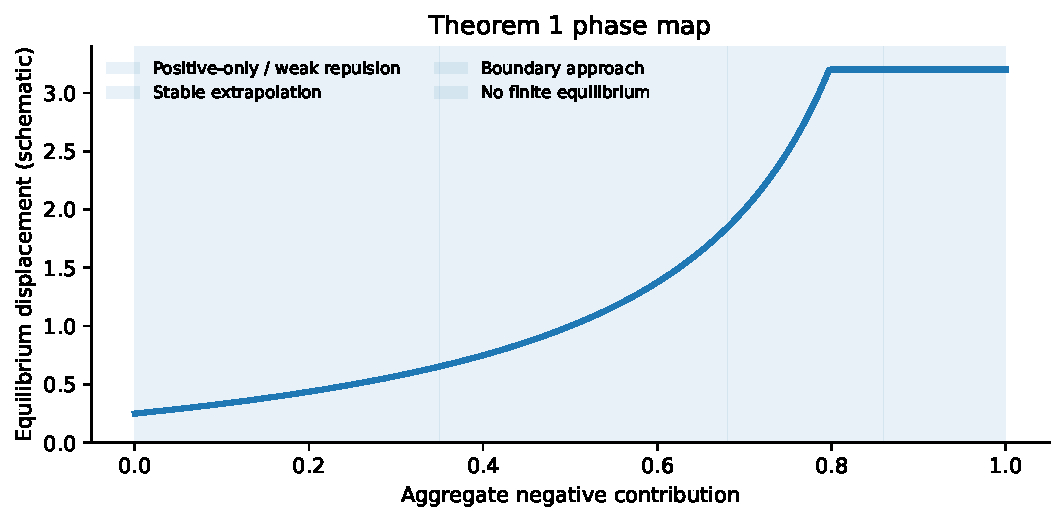
\includegraphics[width=\columnwidth]{figures/generated/fig2_phase_map.pdf}
\caption{Schematic phase map induced by Theorem~\ref{thm:equilibrium}. The empirical tests separately identify the Positive-only target, stable extrapolation, boundary approach, and persistent drift or loss of a finite equilibrium.}
\label{fig:phase-map}
\end{figure}
% END-MANUSCRIPT-NODE: THEORY-P04

% MANUSCRIPT-NODE: THEORY-P05
For Gaussian policies, an interior signed target corresponds to finite mean and covariance parameters; far-field negative updates can increase standardized displacement and contract support, causing score amplification and boundary approach. For categorical policies, an interior target corresponds to finite logits, whereas a boundary target drives selected probabilities toward zero or one. Direct-logit score norms remain bounded, but suppression persists. Thus the transferable principle is aggregate repulsion toward a feasibility boundary, while the local amplification law remains policy-family specific.
% END-MANUSCRIPT-NODE: THEORY-P05

\section{Distributionally Robust Policy Optimization}
\label{sec:method}

% MANUSCRIPT-NODE: METHOD-P01
DRPO applies a policy-relative envelope to the negative component of the signed actor field. Let $r_\theta(s,a)\ge 0$ denote the registered remoteness measure for the policy family and experiment. We define
\begin{equation}
w^-_\lambda(s,a)=\exp[-\lambda r_\theta(s,a)],\qquad \lambda\ge 0,
\label{eq:exp-weight}
\end{equation}
and optimize
\begin{equation}
\mathbf F_{\mathrm{DRPO}}(\theta)=\mathbb E_\nu\!\left[A^+\nabla\log\pi_\theta-A^-w^-_\lambda\nabla\log\pi_\theta\right].
\label{eq:drpo-field}
\end{equation}
Positive updates are unchanged, nearby negative actions retain substantial influence, and increasingly remote negative actions are attenuated. Sample quality and learner-relative remoteness remain distinct axes: the matched experiments vary remoteness without changing badness, while Appendix~\ref{app:optimistic-dro} states the separate Optimistic-DRO quality-selection result. The main DRPO update does not equate the two controls.
% END-MANUSCRIPT-NODE: METHOD-P01

% MANUSCRIPT-NODE: METHOD-P02
In the exponential-family analysis, the uncontrolled negative moment is
\begin{equation}
q\mathbf m_-=\mathbb E[A^-T(a)].
\end{equation}
DRPO replaces it by
\begin{equation}
q_\lambda\mathbf m_{-,\lambda}=\mathbb E[A^-e^{-\lambda r_\theta(s,a)}T(a)],
\label{eq:weighted-negative-moment}
\end{equation}
which induces the controlled target
\begin{equation}
\mathbf m_\lambda^\star=\frac{p\mathbf m_+-q_\lambda\mathbf m_{-,\lambda}}{p-q_\lambda}.
\end{equation}
The method therefore modifies the same term that first creates stable extrapolation and later drives the signed target toward the boundary. Small $r_\theta$ preserves substantial negative influence; large $r_\theta$ is selectively attenuated.
% END-MANUSCRIPT-NODE: METHOD-P02

% MANUSCRIPT-NODE: METHOD-P03
\begin{proposition}[Vanishing weighted far-field gradient]
\label{prop:vanishing}
Suppose the policy score satisfies $\|\nabla_\theta\log\pi_\theta(a\mid s)\|\le C(1+r_\theta(s,a))^k$ for finite $C,k$. For any $\lambda>0$,
\begin{equation}
e^{-\lambda r_\theta(s,a)}\|\nabla_\theta\log\pi_\theta(a\mid s)\|\rightarrow 0
\quad\text{as }r_\theta(s,a)\rightarrow\infty.
\end{equation}
\end{proposition}
The exponential form is therefore a gradient-tail envelope derived from the far-field score-growth bound. Directional utility is measured separately in the controlled experiments.
% END-MANUSCRIPT-NODE: METHOD-P03

% MANUSCRIPT-NODE: METHOD-P04
We compare DRPO against an uncontrolled signed baseline, Positive-only learning, non-selective global scaling, registered linear or reciprocal tapers, and a hard threshold on the same remoteness coordinate. A quality-based hard filter is reported separately because it controls a different axis. Where the protocol calls for budget matching, methods receive the same pre-optimizer raw negative-gradient norm and are evaluated with paired seeds. No method ranking is assumed in advance; best and terminal checkpoints, local-negative retention, far-field retention, task performance, boundary events, and numerical failures are all reported.
% END-MANUSCRIPT-NODE: METHOD-P04

\section{Experiments}
\label{sec:experiments}

% MANUSCRIPT-NODE: EXP-P01
We use two primary controlled environments and two external families. C-U1 is a nonlinear state-conditioned Gaussian environment with six-dimensional numerical contexts, two-dimensional actions, a known state-dependent optimum, and independently sampled train and test contexts from the same distribution. It supports matched quality--distance probes, near/far intervention, and mean--support terminal audits. D-U1 is a shared-network categorical environment with unordered semantic actions and a known reward structure; it supports matched quality--rarity probes, common/rare intervention, and probability-boundary audits. We report C-U1 using the precise term held-out-context or unseen-state generalization. Hopper/D4RL adds a learned critic and long-horizon continuous control, while Countdown adds shared Transformer parameters and sequence-level verification. External tasks establish relevance; controlled environments establish source and causality.

\begin{table*}[t]
\centering
\caption{Evidence roles are separated by design. Controlled environments identify source and causality; external environments establish relevance and task effect.}
\label{tab:environment_roles}
\small
\begin{tabular}{p{0.14\textwidth}p{0.38\textwidth}p{0.38\textwidth}}
\toprule
Environment & Primary responsibility & Complementary boundary \\
\midrule
C-U1 & Continuous matched source isolation, near/far causality, and phase transition & External relevance is established in Hopper/D4RL; categorical boundaries are tested in D-U1 \\
D-U1 & Categorical matched rarity isolation, common/rare causality, and probability boundary & Gaussian score-amplitude dynamics are tested in C-U1 \\
Hopper/D4RL & External continuous-control occurrence and task effect with a learned critic & Exact badness--distance isolation is supplied by C-U1 \\
Countdown & External shared-parameter sequence occurrence and task effect & Controlled common/rare causality is supplied by D-U1 \\
\bottomrule
\end{tabular}
\end{table*}

% END-MANUSCRIPT-NODE: EXP-P01

% MANUSCRIPT-NODE: EXP-P02
\paragraph{Hopper/D4RL.} We train the registered learned critic, freeze its selected checkpoint, and audit negative actor gradients by current-policy distance. The formal report will include far/near negative-gradient ratios, positive/negative imbalance, policy drift, rollout return, and terminal classification. \textbf{TBD:} insert only terminal-audited formal results from the registered E7 package.

\paragraph{Countdown.} We bin negative tokens or completions by current-policy surprisal and track score magnitude, shared-parameter gradient influence, target-probability change, verifier success, validity, and pass@$k$. \textbf{TBD:} insert only the registered formal result; focused pilots remain provenance rather than final evidence.
% END-MANUSCRIPT-NODE: EXP-P02

% MANUSCRIPT-NODE: EXP-P03
The source-isolation protocol holds sample badness fixed. In C-U1, negative actions share the same state, reward, advantage magnitude, quality coordinate, count, coefficient, and policy parameters while varying only learner-relative radius. We report output-space score norms, full-parameter per-sample gradients, aggregate gradients, and directional coherence. In D-U1, common and rare actions are matched in semantic role, reward, negative advantage, count, and base coefficient while initial probability or current surprisal changes. A far/near or rare/common gap under these controls identifies policy remoteness as an independent amplifier; it does not imply that distance is the only factor in real data.
% END-MANUSCRIPT-NODE: EXP-P03
\begin{figure*}[t]
\centering
\begin{subfigure}{0.48\textwidth}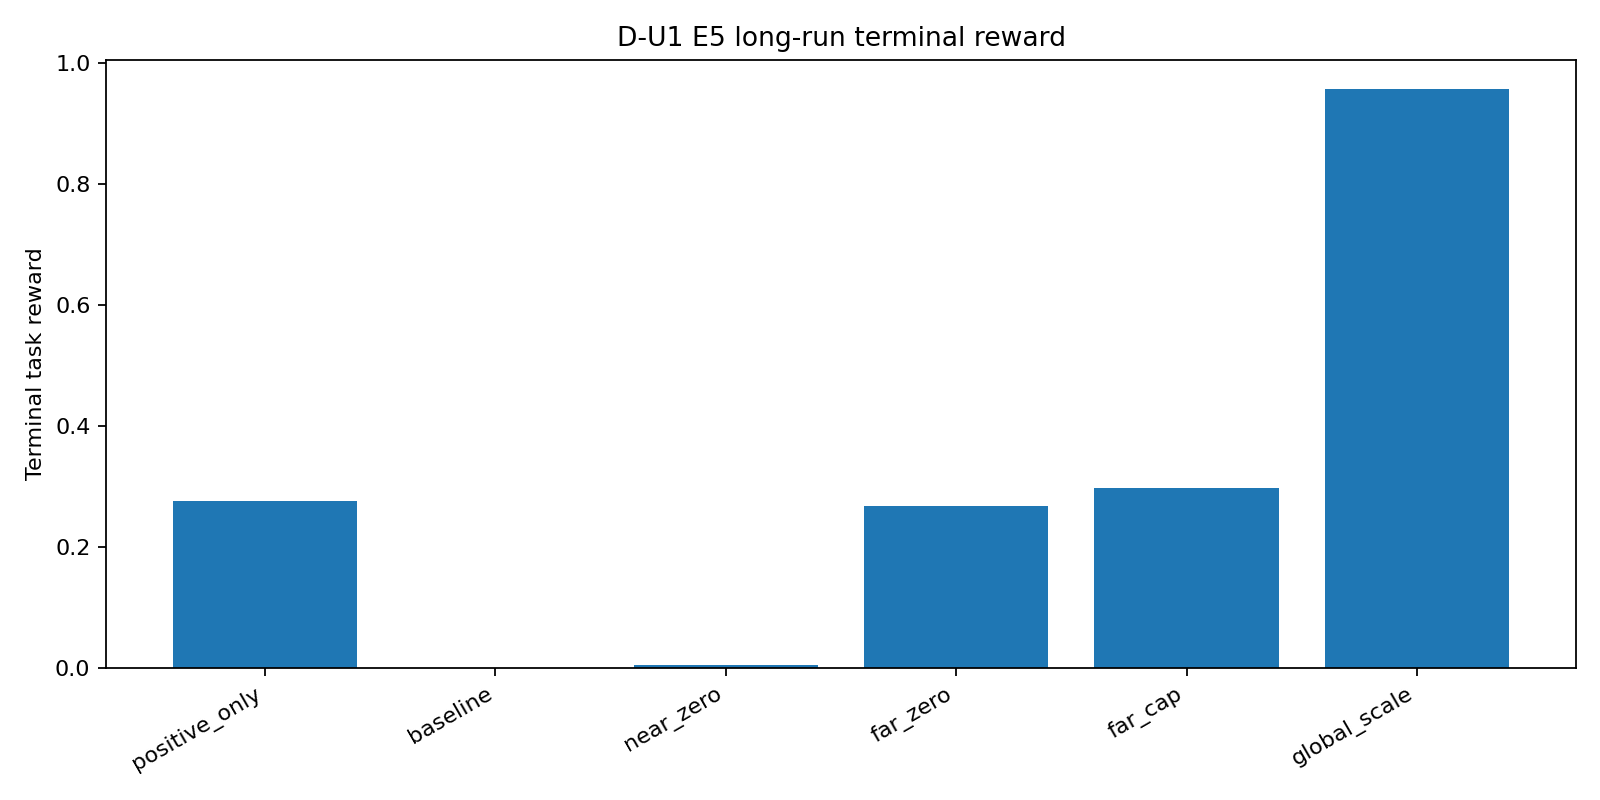
\includegraphics[width=\linewidth]{figures/generated/causal_terminal_reward.png}\caption{Terminal reward.}\end{subfigure}\hfill
\begin{subfigure}{0.48\textwidth}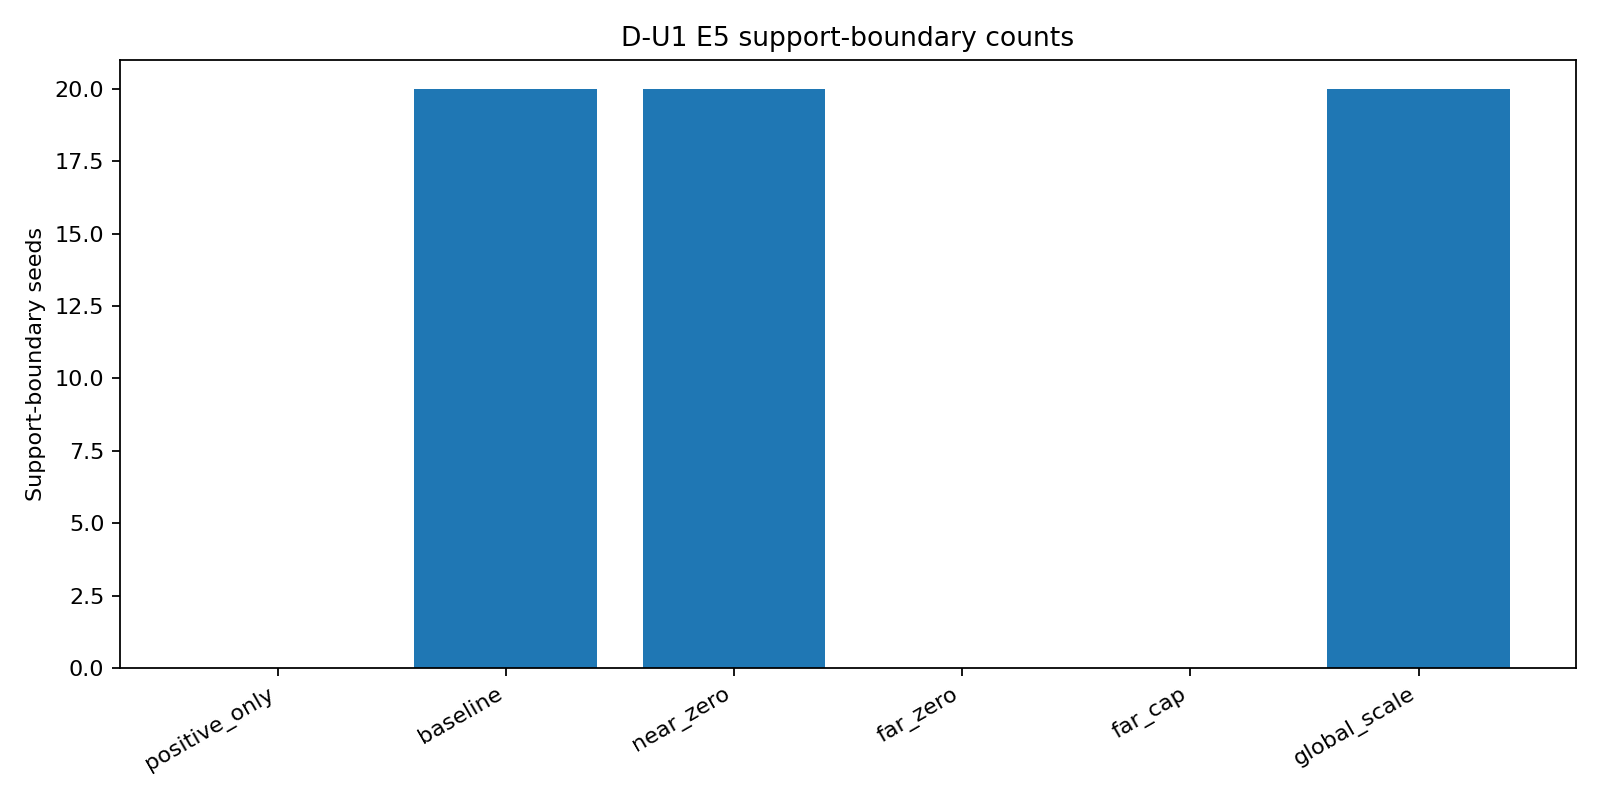
\includegraphics[width=\linewidth]{figures/generated/causal_support_boundary.png}\caption{Support-boundary events.}\end{subfigure}
\caption{D-U1 long-run causal results. Baseline and Near-zero preserve the rare/far negative pathway and reach the support boundary in 20/20 seeds; Far-zero and Far-cap remain bounded in 20/20 seeds. Global scaling can preserve task reward while still reaching the support boundary, illustrating why task, boundary, and numerical events must be reported separately.}
\label{fig:du1-causal}
\end{figure*}
\begin{table}[t]
\centering\small
\caption{D-U1 E5 long-run summary.}
\label{tab:du1-e5}
\begin{tabular}{lccc}
\toprule Method & Reward & Task collapse & Boundary \\
\midrule
baseline & 0.001 & 20/20 & 20/20 \\
near-zero & 0.006 & 20/20 & 20/20 \\
far-zero & 0.267 & 0/20 & 0/20 \\
far-cap & 0.297 & 0/20 & 0/20 \\
global-scale & 0.957 & 0/20 & 20/20 \\
positive-only & 0.275 & 0/20 & 0/20 \\
\bottomrule
\end{tabular}
\end{table}


% MANUSCRIPT-NODE: EXP-P04
We next intervene on the location of negative influence. The continuous comparison includes the uncontrolled signed baseline, Near-zero, Far-zero, Far-cap, a non-selective global control matched to the retained raw negative-gradient budget, and a registered budget-transfer control. The categorical analogue suppresses common or rare negatives under matched counts and budgets. We record the onset order of remote influence, parameter drift, support or probability boundaries, and task performance. A selective far/rare rescue together with an ineffective near/common removal supports the remote component as a causal transmission pathway; task-performance collapse, boundary events, and NaN/Inf remain distinct labels.
% END-MANUSCRIPT-NODE: EXP-P04
\begin{figure*}[t]
\centering
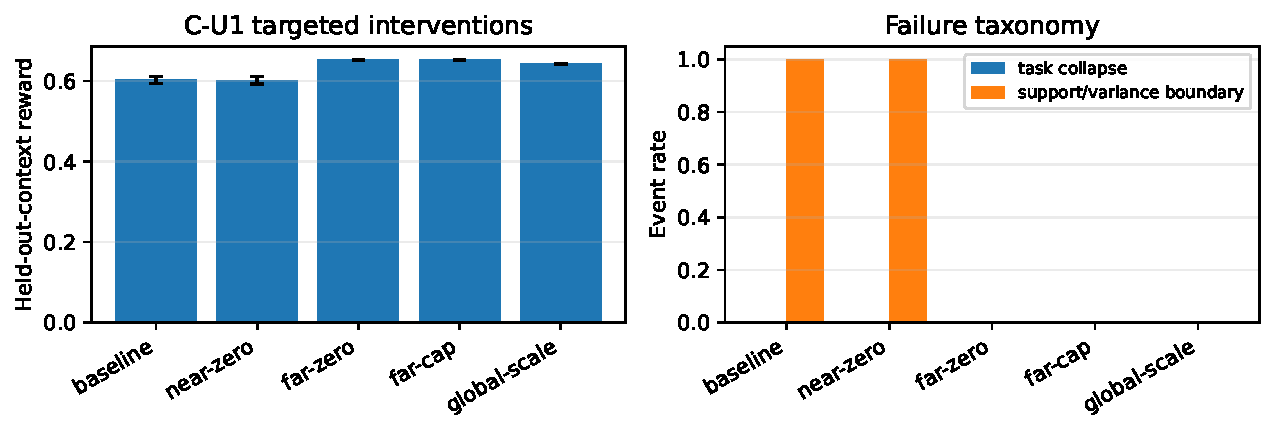
\includegraphics[width=0.93\textwidth]{figures/generated/fig3_cu1_causal.pdf}
\caption{C-U1 causal intervention with learnable variance. The left panel reports registered held-out-context reward with confidence intervals; the right panel separates task-performance collapse from support or variance-boundary events. Near-zero tracks the uncontrolled baseline, while Far-zero and Far-cap remove the task-collapse pathway without introducing NaN/Inf failures.}
\label{fig:cu1-causal}
\end{figure*}
\begin{table}[t]
\centering\small
\caption{C-U1 intervention summary (20 seeds).}
\label{tab:cu1-causal}
\begin{tabular}{lccc}
\toprule Method & Reward & Task event & Boundary event \\
\midrule
baseline & 0.603 & 0.00 & 1.00 \\
near-zero & 0.602 & 0.00 & 1.00 \\
far-zero & 0.653 & 0.00 & 0.00 \\
far-cap & 0.653 & 0.00 & 0.00 \\
global-scale & 0.643 & 0.00 & 0.00 \\
\bottomrule
\end{tabular}
\end{table}


% MANUSCRIPT-NODE: EXP-P05
We sweep the effective negative strength from zero through controlled repulsion and into the unstable regime. The primary test is not a single endpoint score but the phase sequence predicted by Theorem~\ref{thm:equilibrium}: Positive-only, stable extrapolation, boundary approach, and persistent drift or loss of finite equilibrium. We measure a family-specific empirical proxy for the aggregate negative term in~\eqref{eq:weighted-negative-moment}, together with its distance or rarity bins, direction, and relationship to equilibrium displacement. DRPO is compared with Positive-only, global scaling, and registered distance controls under paired seeds and explicit raw-gradient budgets. Results are reported at both selected and terminal checkpoints. \textbf{TBD:} populate the final table only from the current terminal-audited repository artifacts and preserve each result's formal status.

\begin{table*}[t]
\centering
\caption{Controlled phase and method results. Entries remain TBD until the corresponding registered artifacts and terminal audits are frozen for the manuscript. Task collapse, boundary events, and numerical failure are reported separately.}
\label{tab:controlled_results}
\small
\begin{tabular}{lcccccc}
\toprule
Method & Held-out-context reward & Near retention & Far retention & Task collapse & Boundary event & NaN/Inf \\
\midrule
Positive-only & TBD & -- & 0 & TBD & TBD & TBD \\
Uncontrolled signed & TBD & TBD & TBD & TBD & TBD & TBD \\
Global matched & TBD & TBD & TBD & TBD & TBD & TBD \\
Hard distance control & TBD & TBD & TBD & TBD & TBD & TBD \\
DRPO exponential & TBD & TBD & TBD & TBD & TBD & TBD \\
\bottomrule
\end{tabular}
\end{table*}

% END-MANUSCRIPT-NODE: EXP-P05
\begin{figure*}[t]
\centering
\begin{subfigure}{0.62\textwidth}
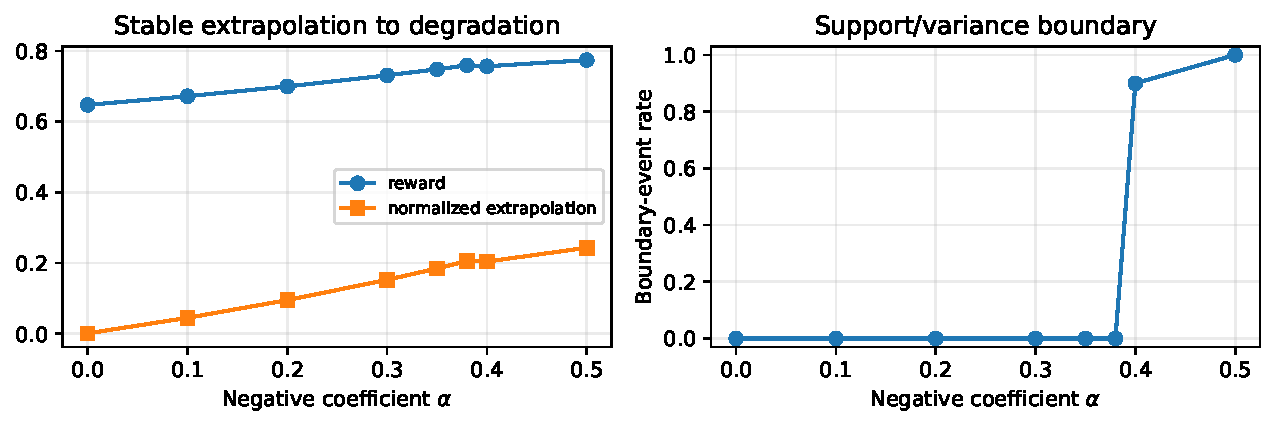
\includegraphics[width=\linewidth]{figures/generated/fig4_cu1_phase.pdf}
\caption{Strength sweep and boundary events.}
\end{subfigure}\hfill
\begin{subfigure}{0.34\textwidth}
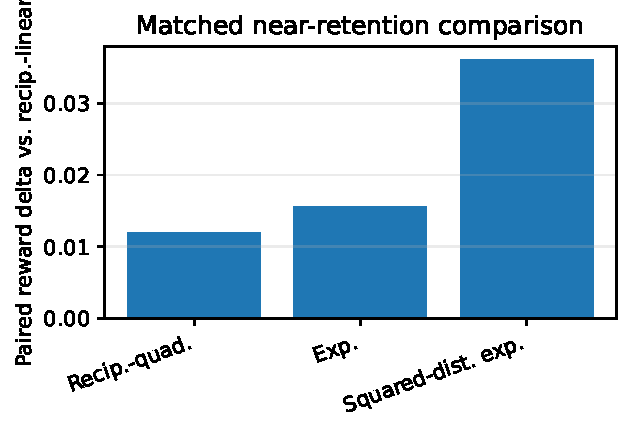
\includegraphics[width=\linewidth]{figures/generated/fig5_taper_shape.pdf}
\caption{Matched near-retention taper comparison.}
\end{subfigure}
\caption{C-U1 phase and control evidence. The strength sweep maps the transition from the Positive-only reference through stable extrapolation toward boundary events. Under the frozen near-retention protocol, all three faster-decaying tapers improve finite-horizon held-out-context reward on 20/20 paired seeds relative to reciprocal-linear; this result remains finite-step validated rather than a universal steady-state ranking.}
\label{fig:cu1-phase-control}
\end{figure*}


% MANUSCRIPT-NODE: EXP-P06
The final evaluation returns to external tasks. On D4RL locomotion, methods share dataset, critic protocol, initialization, seeds, evaluation horizon, and selection rule; we report normalized return, uncertainty, best and terminal checkpoints, and distance-binned negative influence. On Countdown, methods share the SFT initialization, rollout or replay bank, verifier, seeds, and checkpoint-selection protocol; we report greedy success, pass@$k$, validity, terminal degradation, and rare-negative diagnostics. \textbf{TBD:} the main external tables remain unfilled until the corresponding registered formal experiments are terminal-audited and delivered.

\begin{table*}[t]
\centering
\caption{External task closure. Best and terminal results are both required; no values are inserted before formal terminal-audited completion.}
\label{tab:external_results}
\small
\begin{tabular}{llccccc}
\toprule
Family & Dataset/model & Uncontrolled & Positive-only & Global & DRPO & Terminal failure rate \\
\midrule
D4RL & Hopper / locomotion suite & TBD & TBD & TBD & TBD & TBD \\
Countdown & Main model scale & TBD & TBD & TBD & TBD & TBD \\
\bottomrule
\end{tabular}
\end{table*}

% END-MANUSCRIPT-NODE: EXP-P06

\section{Implications and Conclusion}
\label{sec:conclusion}

% MANUSCRIPT-NODE: DISC-P01
Negative feedback is a policy-improvement resource with a dynamical failure mode. It provides boundary information and can shift a policy beyond the Positive-only target. The failure arises when historical actions remain active after becoming remote from the current learner, so their optimization influence no longer tracks their local relevance. The transferable design principle is therefore to control learner-relative far-field negative influence rather than delete negative feedback as a class.
% END-MANUSCRIPT-NODE: DISC-P01

% MANUSCRIPT-NODE: DISC-P02
The continuous and categorical analyses share an aggregate structure but not an identical local law. Gaussian policies can amplify mean scores with standardized distance and couple repulsion to support contraction. Categorical direct-logit scores remain bounded, yet repeated negative updates can persistently suppress probability. In both cases, aggregate positive--negative competition determines whether the policy remains at an interior equilibrium or moves toward a feasibility boundary.
% END-MANUSCRIPT-NODE: DISC-P02

% MANUSCRIPT-NODE: DISC-P03
Negative feedback can create stable policy improvement beyond Positive-only learning. By separating badness from policy remoteness, we identify how historical negative actions become far-field, dominate the aggregate update, and move the policy toward a feasibility boundary where a finite equilibrium can disappear. DRPO controls this same negative term, preserving useful local repulsion while suppressing the destructive far-field tail.
% END-MANUSCRIPT-NODE: DISC-P03


\bibliography{references}
\bibliographystyle{icml2026}

\clearpage
\appendix
\section{Proofs for Repulsive Dynamics}
\label{app:proofs}

% MANUSCRIPT-NODE: APP-PROOF-P01
For a regular minimal exponential family, $\nabla\psi$ maps the natural-parameter space diffeomorphically onto the interior of the mean-parameter space. Setting~\eqref{eq:aggregate-field} to zero with $p>q$ gives~\eqref{eq:signed-target}. If $\mathbf m^\star$ is interior, uniqueness follows from strict convexity of $\psi$. The displacement identity follows by subtracting $\mathbf m_+$ from~\eqref{eq:signed-target}. If $\mathbf m^\star$ approaches the boundary, no finite natural parameter realizes it; if it lies outside the closure, no policy in the family realizes the target. Differentiating~\eqref{eq:aggregate-field} gives $J_F=-(p-q)\nabla^2\psi$, which is negative definite at an interior point because the Hessian is the positive-definite covariance of the sufficient statistic. The discrete update is locally stable for step sizes whose transition matrix has spectral radius below one.
% END-MANUSCRIPT-NODE: APP-PROOF-P01

\subsection{Detailed derivation for Theorem~\ref{thm:equilibrium}}
\label{app:proof-theorem-equilibrium}
\begin{proof}
Let $F(\eta)=p(\mathbf m_+-\nabla\psi(\eta))-q(\mathbf m_--\nabla\psi(\eta))$. Rearranging gives
\begin{equation}
F(\eta)=p\mathbf m_+-q\mathbf m_--(p-q)\nabla\psi(\eta).
\end{equation}
For $p>q$, $F(\eta)=0$ is equivalent to
\begin{equation}
\nabla\psi(\eta)=\mathbf m^\star=\frac{p\mathbf m_+-q\mathbf m_-}{p-q}.
\end{equation}
A regular minimal exponential family has strictly convex log-partition $\psi$, so $\nabla\psi$ is one-to-one and maps the natural-parameter space onto the interior of the realizable mean-parameter set. Hence an interior $\mathbf m^\star$ has a unique finite preimage $\eta^\star$. Subtracting $\mathbf m_+$ yields
\begin{equation}
\mathbf m^\star-\mathbf m_+=\frac{q}{p-q}(\mathbf m_+-\mathbf m_-),
\end{equation}
which is the stable extrapolation displacement. Differentiating the field gives
\begin{equation}
J_F(\eta)=-(p-q)\nabla^2\psi(\eta).
\end{equation}
At $\eta^\star$, $\nabla^2\psi$ is the covariance of the sufficient statistic and is positive definite; therefore every eigenvalue of $J_F$ is negative and the continuous-time equilibrium is locally asymptotically stable. For discrete step size $h$, local stability requires $\rho(I+hJ_F)<1$. If $\mathbf m^\star$ reaches the feasible boundary, the realizing natural parameter diverges or becomes degenerate; outside the feasible set, no finite equilibrium exists.
\end{proof}

\subsection{Proof of Proposition~\ref{prop:vanishing}}
\label{app:proof-far-field}
\begin{proof}
Assume the unweighted score satisfies $\|\nabla_\theta\log\pi_\theta(a\mid s)\|\le C(1+r_\theta)^k$ for finite $k$, and let $w_\lambda(r)=\exp(-\lambda r^2)$. Then
\begin{equation}
\|w_\lambda(r)A^-\nabla_\theta\log\pi_\theta\|
\le |A^-|C(1+r)^k e^{-\lambda r^2}.
\end{equation}
For every finite $k$ and $\lambda>0$, the Gaussian tail dominates the polynomial factor, so the right-hand side converges to zero as $r\to\infty$. This proves vanishing weighted far-field influence without assuming that the sample's utility decays exponentially.
\end{proof}


\section{Gaussian Mean--Variance Derivations}
\label{app:gaussian}

% MANUSCRIPT-NODE: APP-GAUSS-P01
For a scalar Gaussian with $\xi=\log\sigma$ and $z=(a-\mu)/\sigma$,
\begin{equation}
\partial_\mu\log\pi=\frac{a-\mu}{\sigma^2},\qquad
\partial_\xi\log\pi=z^2-1.
\end{equation}
A negative advantage reverses both score directions. It always pushes the mean away from the action, but its effect on scale depends on $|z|$: a near negative action with $|z|<1$ increases $\sigma$, whereas a far negative action with $|z|>1$ decreases $\sigma$. Positive updates have the opposite signs. A full Gaussian terminal state must satisfy both mean and variance equations; a stationary mean with continuing covariance movement is not a complete policy equilibrium.
% END-MANUSCRIPT-NODE: APP-GAUSS-P01

\subsection{Population mean--variance fixed point}
With $\xi=\log\sigma$, positive mass $p$, effective negative mass $q$, conditional moments $(m_+,v_+)$ and $(m_-,v_-)$,
\begin{align}
\dot\mu &= \frac{p(m_+-\mu)-q(m_--\mu)}{\sigma^2},\\
\dot\xi &= \frac{p[v_++(\mu-m_+)^2]-q[v_-+(\mu-m_-)^2]}{\sigma^2}-(p-q).
\end{align}
For $p>q$, the mean candidate is $\mu^\star=(pm_+-qm_-)/(p-q)$. Substitution into the scale equation gives
\begin{equation}
(\sigma^2)^\star=\frac{pM_+(\mu^\star)-qM_-(\mu^\star)}{p-q},
\end{equation}
where $M_\pm(\mu)=v_\pm+(\mu-m_\pm)^2$. A finite joint equilibrium therefore requires both $p>q$ and a positive numerator. This second condition is stricter in the far field because $M_-$ contains squared displacement.


\section{Categorical Boundary Dynamics}
\label{app:categorical}

% MANUSCRIPT-NODE: APP-CAT-P01
For softmax probabilities $p_j$, the score for selected action $y$ is $e_y-p$, whose Euclidean norm is bounded. Under a negative update with fixed local coefficient, the selected logit decreases relative to competing logits, so $z_y-z_j$ falls approximately linearly while $p_y$ can decay exponentially. The failure mode is therefore persistent support suppression toward the simplex boundary. In a shared network, the parameter-space gradient additionally contains the network Jacobian and cross-action interference, which are measured rather than inferred from the direct-logit bound alone.
% END-MANUSCRIPT-NODE: APP-CAT-P01

\subsection{Repeated negative updates and log-odds}
For softmax logits $z$, $\nabla_z\log p_y=e_y-p$. Under a fixed negative coefficient $c>0$ and small step size $h$, the selected logit changes by $-hc(1-p_y)$ while competitor $j$ changes by $+hc p_j$. Hence
\begin{equation}
(z_y-z_j)_{t+1}-(z_y-z_j)_t=-hc(1-p_y+p_j),
\end{equation}
which remains negative as $p_y\to0$. The Euclidean score is bounded, but the non-vanishing log-odds decrement yields persistent support suppression and can drive $p_y$ exponentially toward the simplex boundary.


\section{Controlled Environments}
\label{app:environments}

% MANUSCRIPT-NODE: APP-ENV-P01
C-U1 samples numerical contexts $s\sim\mathcal N(0,I_6)$ independently for training and testing. A fixed generator maps each state to a positive action, hidden optimal action, negative quality coordinate, and reward surface in $\mathbb R^2$. Source-isolation probes replicate reward and advantage across radii while retaining the same state and quality coordinate. Near/far membership for causal interventions is computed relative to the current policy according to the registered metric. D-U1 uses a shared state-conditioned categorical network over unordered semantic actions; quality/semantics and rarity are factorized so that common/rare probes can be matched in reward, advantage, count, and coefficient. Complete constants, seeds, and invariants are taken from the registered experiment configurations.
% END-MANUSCRIPT-NODE: APP-ENV-P01

\section{Experimental Protocols and Terminal Audits}
\label{app:protocols}

% MANUSCRIPT-NODE: APP-PROT-P01
Formal protocols specify maximum horizons, evaluation cadence, paired development and held-out seeds, and a terminal audit before execution. A fixed horizon is not itself called convergence. Depending on the registered experiment, terminal classification uses state slopes, update residuals, boundary checks, and a continuation horizon. Budget-matched comparisons use the pre-optimizer raw negative-gradient $\ell_2$ norm unless another coordinate is explicitly frozen. Adam parameter-update norms are recorded separately. Best-validation and terminal checkpoints are both reported, and task-performance collapse, support or variance boundaries, and NaN/Inf failures remain distinct fields.
% END-MANUSCRIPT-NODE: APP-PROT-P01

\section{Additional Results and Failure Taxonomy}
\label{app:results}

% MANUSCRIPT-NODE: APP-RES-P01
This appendix will contain per-seed results, full training trajectories, confidence intervals, sensitivity analyses, and terminal classifications for every main comparison. Failed or inconclusive formal runs are indexed rather than silently removed. \textbf{TBD:} populate these materials from the durable formal packages after repository closure; smoke tests, static checks, and focused pilots are not promoted to formal evidence.
% END-MANUSCRIPT-NODE: APP-RES-P01

\section{Implementation and Reproducibility}
\label{app:repro}

% MANUSCRIPT-NODE: APP-REPRO-P01
The repository records experiment IDs, configurations, seeds, code entry points, result manifests, raw curves, logs, terminal audits, checksums, and source commits. Formal runs progress through registered, running, raw-complete, terminal-audited, packaged, delivered, and applied states. The paper source is generated from the stable-ID manuscript graph, compiled in the imported ICML/Overleaf project, and packaged with a reproducible build command. Exact repository paths and commit hashes will be inserted at submission freeze.
% END-MANUSCRIPT-NODE: APP-REPRO-P01

\section{Optimistic Distributional Selection}
\label{app:optimistic-dro}

% MANUSCRIPT-NODE: APP-DRO-P01
Let $P$ denote the empirical data distribution and let $R(s,a)$ be the registered quality signal. The Optimistic-DRO selection problem is
\begin{equation}
\begin{aligned}
\max_Q\quad &\mathbb E_Q[R(s,a)]\\
\text{s.t.}\quad &Q\ll P,\qquad 0\le \frac{dQ}{dP}\le \frac{1}{\kappa},\\
&\int dQ=1.
\end{aligned}
\label{eq:optimistic-dro}
\end{equation}
Its optimum allocates the maximum admissible density to the highest-quality region of $P$, with boundary mass only when needed to satisfy normalization. For a continuous reward distribution this is the top-$\kappa$ hard-selection solution. This result establishes a principled quality-selection operator inside the current DRPO manuscript. It does not identify policy remoteness with low quality and does not derive the exponential envelope in Eq.~\eqref{eq:exp-weight}. Quality selection controls which data are emphasized; remoteness tapering controls how a negative sample's influence changes as the learner moves. The source-isolation experiments keep quality fixed precisely so that the second effect can be identified independently.
% END-MANUSCRIPT-NODE: APP-DRO-P01

\section{Additional Theoretical and Reporting Clarifications}
\label{app:corrections}

% MANUSCRIPT-NODE: APP-CORR-P01
The manuscript uses the following technical conventions throughout. Far-field negative Gaussian updates combine mean repulsion with location-dependent scale dynamics and commonly support contraction; they do not universally expand both mean and variance. The expected Fisher matrix describes policy geometry but does not by itself determine stability of a fixed off-policy signed field; local stability is evaluated with the Jacobian of the actual aggregate field. C-U1 test states are independently sampled from the same state distribution and are described as held-out-context or unseen-state generalization, not OOD generalization. Task-performance collapse, support or variance boundaries, and NaN/Inf numerical failure are reported separately. Finally, finite-horizon evidence is not relabeled as convergence or long-run validation without the registered terminal audit.
% END-MANUSCRIPT-NODE: APP-CORR-P01

\end{document}
